%\documentclass[letterpaper,12pt]{article}
\documentclass{article}
\usepackage{graphicx} % Required for inserting images
\usepackage{amsmath}
\usepackage[table,xcdraw,dvipsnames]{xcolor}
\usepackage{animate}   % <- paquete clave
%\usepackage[hidelinks]{hyperref}
\usepackage{textcomp}
\usepackage{colortbl}
\usepackage{amssymb}
\usepackage{float}
\usepackage{enumitem}
\usepackage[normalem]{ulem}
\useunder{\uline}{\ul}{}
\usepackage{titletoc}
\usepackage{csquotes}
\usepackage{listings}
\usepackage{booktabs}
\usepackage{multirow}
\usepackage{relsize}

\usepackage{fancyhdr}

\setlength{\headheight}{14pt} % evita warnings con fancyhdr
\pagestyle{fancy}
\fancyhf{}                   % limpia encabezado/pie
\fancyhead[R]{\thepage}      % número de página arriba a la derecha
\renewcommand{\headrulewidth}{0pt} % sin línea

\lstset{basicstyle=\ttfamily\small, breaklines=true, frame=single}

\usepackage[spanish,english]{babel} % carga ambos idiomas
\addto\captionsspanish{
    \renewcommand{\tablename}{Tabla}
    \renewcommand{\listtablename}{Índice de tablas}
}

\usepackage[
    colorlinks=true,    % enlaces como texto coloreado
    linkcolor=black,    % color de los enlaces internos (índice)
    citecolor=black,    % color de las citas
    urlcolor=black,     % color de las urls
    filecolor=black     % color de los enlaces a archivos
]{hyperref}
\newfloat{imagen}{H}{loi}
\floatname{imagen}{Imagen}
\newcommand{\listofimages}{\listof{imagen}{Índice de imágenes}}

%\documentclass{article}
%\title{Protocolo de Investigación - Pronóstico de la Inflación en México - Una comparación de métodos clásicos, Arboles de Decisión y Redes Neuronales}

\begin{document}

\thispagestyle{empty}
\begin{figure}[h]
    \centering
    \begin{minipage}{.25\textwidth}
        \centering
        
\includegraphics[width=.8\linewidth]{portada/uaq_logo.jpg}
    \end{minipage}%
    \begin{minipage}{.25\textwidth}
        \centering
        
\includegraphics[width=.8\linewidth]{portada/ING_LOGO_UAQ.png}
    \end{minipage}
\end{figure}

%\hfill
\begin{center}
    \centering
    {\Large \textbf{UNIVERSIDAD AUTÓNOMA DE QUERÉTARO}}\\[0.4cm]
    {\Large \textbf{FACULTAD DE INGENIERÍA}}
\end{center}

\vspace{1cm}
\begin{center}
    {\bfseries \large Predicción de la Inflación en México:}\\[0.1cm]
    {\bfseries \large Un Estudio Comparativo entre Modelos Clásicos, Árboles de Decisión y Redes Neuronales}\\[0.6cm]

    {\Large \textbf{TESIS}}\\[0.6cm]
    {\small \textbf{PARA OBTENER EL TÍTULO DE}}\\[0.3cm]
    {\large \textbf{LICENCIATURA EN MATEMÁTICAS APLICADAS}}\\[1.2cm]

    {\small \textbf{PRESENTA}}\\[0.3cm]
    {\large \textbf{Norberto Peña Rodríguez}}\\[1.2cm]

    {\small \textbf{DIRIGIDA POR}}\\[0.3cm]
    {\large \textbf{Dr. Víctor Antonio Aguilar Arteaga}}%
\end{center}

\newpage
% ---------- LOGO ----------
\thispagestyle{empty}
\begin{figure}[h]
    \centering
    \begin{minipage}{.25\textwidth}
        \centering
        
\includegraphics[width=.7\linewidth]{portada/uaq_logo.jpg}
    \end{minipage}%
    \begin{minipage}{.25\textwidth}
        \centering
        
\includegraphics[width=.7\linewidth]{portada/ING_LOGO_UAQ.png}
    \end{minipage}
\end{figure}
\hfill
\begin{center}
    \centering
    {\large \textbf{UNIVERSIDAD AUTÓNOMA DE QUERÉTARO}}\\[0.4cm]
    {\large \textbf{FACULTAD DE INGENIERÍA}}
\end{center}

\vspace{.25cm}
\begin{center}
    {\bfseries \large Predicción de la Inflación en México:}\\[0.1cm]
    {\bfseries \large Un Estudio Comparativo entre Modelos Clásicos, Árboles de Decisión y Redes Neuronales}\\[0.6cm]

    {\Large \textbf{TESIS}}\\[0.3cm]
    {\small \textbf{PARA OBTENER EL TÍTULO DE}}\\[0.3cm]
    {\large \textbf{LICENCIATURA EN MATEMÁTICAS APLICADAS}}\\[1cm]

    {\small \textbf{PRESENTA}}\\[0.1cm]
    {\large \textbf{Norberto Peña Rodríguez}}\\[1cm]

    {\small \textbf{DIRIGIDA POR}}\\[0.1cm]
    {\large \textbf{Dr. Víctor Antonio Aguilar Arteaga}}%
\end{center}

\vspace{.5cm}

% ---------- SINODALES ----------
{\setlength{\extrarowheight}{6pt}
\noindent
\begin{tabular*}{\textwidth}{@{}p{0.55\textwidth}@{\extracolsep{\fill}}p{0.35\textwidth}@{}}
Dr. Víctor Antonio Aguilar Arteaga\\
Presidente
&
\makebox[0.35\textwidth]{\hrulefill}
\\
M en C Iván González García\\
Secretario
&
\makebox[0.35\textwidth]{\hrulefill}
\\
Dr. Francisco Gerardo Jiménez López\\
Vocal
&
\makebox[0.35\textwidth]{\hrulefill}
\\
M.C. Juan Pablo Ramrez Vazquez\\
Suplente
&
\makebox[0.35\textwidth]{\hrulefill}
\end{tabular*}
}

\newpage
\pagenumbering{roman}

\clearpage
\phantomsection
\addcontentsline{toc}{section}{Abstract}
\selectlanguage{english}
\begin{abstract}
Inflation constitutes one of the most complex economic phenomena to model, due to its dynamic
and nonlinear nature, as well as the presence of structural and stochastic components that
evolve over time. In this research, a forecasting system for inflation in Mexico is developed,
integrating classical methodologies, machine learning algorithms, and deep learning models,
with the objective of comparing their performance, stability, and generalization capability
under different validation schemes.

The study proposes a unified framework that automates training, validation, and forecasting
through Bayesian optimization and cross-validation, applicable to different forecasting
horizons. Models ranging from Holt--Winters triple exponential smoothing and XGBoost to advanced
architectures such as RNN, LSTM, DeepAR, Transformer, and D\textsuperscript{3}VAE are implemented,
exploring how each approach captures the seasonality, trend, and nonlinearity inherent in the
inflationary process.

The results show that, although deep neural networks can fit the observed inflation dynamics
with high accuracy, their performance is not consistent across all scenarios, exhibiting
higher variance under cross-validation, particularly when incorporating temporal exogenous
variables and signals derived from the Fourier Transform. In contrast, attention-based models
and probabilistic generative approaches, particularly Transformer and
D\textsuperscript{3}VAE, exhibit a better balance between accuracy and stability, achieving the
best performance in medium- and long-term forecasting horizons.

Finally, the study demonstrates that simple statistical models, such as the historical average
and the naive forecast based on the last observed value, constitute surprisingly competitive
baselines due to their low variance and robustness. These findings underscore that the use of
complex models does not inherently guarantee superior results, and highlight the importance of
combining statistical techniques and deep learning within a systematic, explainable, and
scalable framework for the analysis and monitoring of inflation at the national level.

\vspace{0.4cm}
\noindent\textbf{Keywords:} Inflation in Mexico; time series forecasting; machine learning; deep learning; Bayesian optimization.
\end{abstract}

\clearpage
\phantomsection
\addcontentsline{toc}{section}{Resumen}
\selectlanguage{spanish}
\begin{abstract}
La inflación constituye uno de los fenómenos económicos más complejos de modelar, debido a su
naturaleza dinámica, no lineal y a la presencia de componentes estructurales y estocásticos que
varían en el tiempo. En esta investigación se desarrolla un sistema de predicción para la
inflación en México, integrando metodologías clásicas, algoritmos de aprendizaje automático y
modelos de aprendizaje profundo, con el objetivo de comparar su desempeño, estabilidad y
capacidad de generalización bajo distintos esquemas de validación.

El estudio propone un marco unificado que automatiza el entrenamiento, validación y pronóstico
mediante optimización Bayesiana y validación cruzada, aplicable a distintos horizontes
temporales. Se implementan modelos desde el suavizado exponencial triple de Holt--Winters y
XGBoost, hasta arquitecturas avanzadas como RNN, LSTM, DeepAR, Transformer y
D\textsuperscript{3}VAE, explorando cómo cada enfoque captura la estacionalidad, tendencia y no
linealidad inherentes al proceso inflacionario.

Los resultados muestran que, si bien las redes neuronales profundas pueden ajustarse con gran
precisión a la dinámica observada de la inflación, su desempeño no es consistente en todos los
escenarios, presentando una mayor varianza bajo validación cruzada, particularmente al
incorporar variables exógenas temporales y señales derivadas de la Transformada Discreta de
Fourier. En contraste, los modelos basados en atención y los enfoques generativos
probabilísticos, en particular Transformer y D\textsuperscript{3}VAE, exhiben un mejor balance
entre precisión y estabilidad, logrando el mejor desempeño en horizontes de mediano y largo
plazo.

Finalmente, el estudio evidencia que modelos estadísticos simples, como el promedio histórico
y el pronóstico ingenuo basado en el último valor observado, constituyen líneas base
sorprendentemente competitivas, debido a su baja varianza y robustez. Estos hallazgos subrayan
que el uso de modelos complejos no garantiza mejores resultados, y resaltan la importancia de
combinar técnicas estadísticas y de aprendizaje profundo dentro de un marco sistemático,
explicable y escalable para el análisis y seguimiento de la inflación a nivel nacional.

\vspace{0.4cm}
\noindent\textbf{Palabras clave:} Inflación en México; pronóstico de series temporales; aprendizaje automático; aprendizaje profundo; optimización bayesiana.
\end{abstract}



\newpage

\clearpage
\phantomsection
\addcontentsline{toc}{section}{Dedicatoria}
\section*{Dedicatoria}

A mis padres y a mi familia, porque antes de cualquier logro, modelo, resultado o título,
existió su presencia. Porque en los momentos en los que dudé de mí, de mi camino o de mi
capacidad para terminar lo que había comenzado, su amor siguió siendo una forma silenciosa
de sostén. Esta tesis también les pertenece, porque mucho de lo que soy nació de su esfuerzo,
de su paciencia y de su manera de acompañarme incluso cuando yo mismo no sabía explicar lo
que estaba viviendo.

A mis amigos, especialmente a quienes permanecieron en las buenas y en las malas. A quienes
me escucharon, me cuestionaron, me hicieron reír, me confrontaron y, sin darse cuenta, me
recordaron que uno no se construye solo. En cada conversación profunda, en cada consejo, en
cada momento compartido, hubo una parte de mí que aprendió a mirar la vida con más claridad.

A Castaño, por las ideas, las discusiones y las referencias compartidas; por recordarme que
el conocimiento también se forma en el diálogo, en la curiosidad y en la disposición de mirar
un problema desde otro lugar.

A Víctor, mi director de tesis, por abrirme la puerta a este tema, por orientarme con libertad
y por permitirme desarrollar una investigación que terminó siendo mucho más que un requisito
académico. Gracias por ayudarme a encontrar en la inflación, en los modelos y en los datos,
una forma distinta de pensar el mundo.

Dedico también este trabajo a todas las personas que, aun sin permanecer para siempre,
dejaron algo en mí. A quienes me inspiraron, a quienes me enseñaron
que crecer también implica perder, cambiar, soltar y volver a empezar. Hay personas que pasan
por la vida como estrellas fugaces, que iluminan nuestras vidas en un abrir y cerrar de ojos; otras, como una respuesta; y otras, simplemente como un recordatorio de lo lindo que es vivir y contribuir significativamente a este mundo. Todas ellas, de alguna forma, me trajeron hasta aquí.

Finalmente, dedico esta tesis a esa parte de mí que siguió buscando sentido en las matemáticas, en la ciencia, en el arte, en el trabajo, en el amor y en la posibilidad de ser mejor. Esta tesis es testimonio de ese camino.

\newpage



\clearpage
\phantomsection
\addcontentsline{toc}{section}{Agradecimientos}
\section*{Agradecimientos}
Quiero expresar mi más sincero agradecimiento a mis padres y a mi familia, por su apoyo
constante, comprensión y acompañamiento a lo largo de mi formación académica y personal.
Su respaldo ha sido fundamental para la culminación de este trabajo.
Agradezco también a mis amigos, quienes a través del diálogo, la reflexión y el
cuestionamiento continuo han contribuido a ampliar mi forma de pensar y de entender el
mundo.
Un agradecimiento especial a Castaño, por la información, discusiones y referencias
compartidas, las cuales resultaron valiosas durante el desarrollo de esta investigación.
Asimismo, expreso mi gratitud a Víctor, mi director de tesis, por su apertura, orientación
y por incentivar mi interés en el estudio de este tema, lo que derivó en un acercamiento
más profundo al análisis económico y financiero.
Finalmente, agradezco a todas las personas que, de una u otra forma, formaron parte de
este proceso y contribuyeron a mi crecimiento personal y académico.


\newpage

\clearpage
\phantomsection
\addcontentsline{toc}{section}{Abreviaturas y siglas}
\section*{Abreviaturas y siglas}

\begin{description}[leftmargin=3cm, style=nextline]
    \item[Banxico] Banco de México.
    \item[INEGI] Instituto Nacional de Estadística y Geografía.
    \item[IPC] Índice Nacional de Precios al Consumidor.
    \item[DFT] Transformada Discreta de Fourier.
    \item[KL] Divergencia de Kullback--Leibler.
    \item[MAE] Error absoluto medio.
    \item[RMSE] Raíz del error cuadrático medio.
    \item[MAPE] Error porcentual absoluto medio.
    \item[XGBoost] Extreme Gradient Boosting.
    \item[RNN] Red neuronal recurrente.
    \item[LSTM] Long Short-Term Memory.
    \item[DeepAR] Modelo autorregresivo profundo probabilístico.
    \item[VAE] Autoencoder variacional.
    \item[D\textsuperscript{3}VAE] Modelo variacional basado en procesos de difusión para series temporales.
\end{description}


\clearpage
\thispagestyle{empty}
\begin{figure}[p]
    \centering
    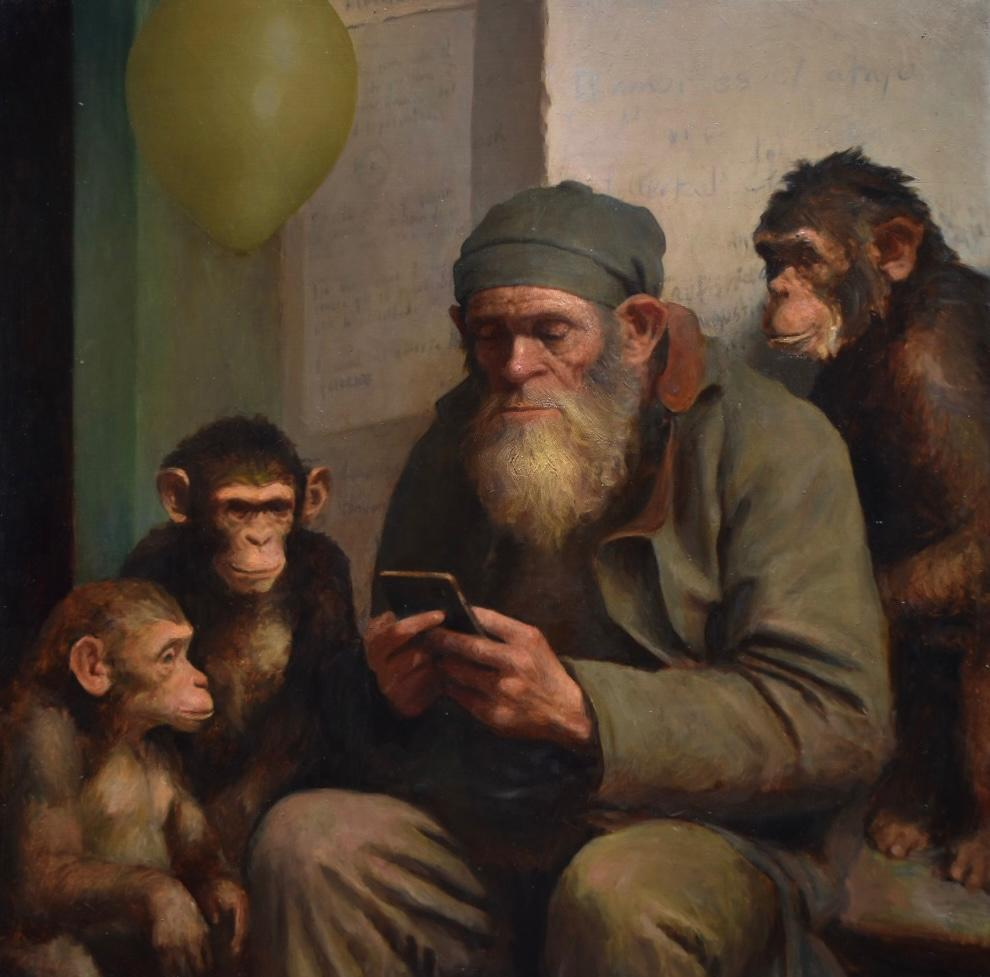
\includegraphics[width=0.9\textwidth]{pinturas/nacho_paint.jpeg} % nombre del archivo
    \addcontentsline{loi}{imagen}{Autodeterminismo del Free Fire, Ignacio Chávez (2025)}
    \caption*{
    \textbf{Autodeterminismo del Free Fire}\\
    Autor: Ignacio Chávez (2025).\\
    Técnica: Óleo sobre lino \\
    Medidas: 90cm x 90cm \\
    Fuente: Cortesía del autor.
    }
\end{figure}

\clearpage

\clearpage
\phantomsection
\addcontentsline{toc}{section}{Índice general}
\tableofcontents

\clearpage
\phantomsection
\addcontentsline{toc}{section}{Índice de cuadros}
\listoftables

\clearpage
\phantomsection
\addcontentsline{toc}{section}{Índice de figuras}
\listoffigures

\clearpage
\phantomsection
\addcontentsline{toc}{section}{Índice de imágenes}
\listofimages


\clearpage
\pagenumbering{arabic}



\pagenumbering{arabic}

%%\section*{\Large Capitulo 1}
\section{Introducción}
En un contexto económico caracterizado por alta volatilidad y constantes perturbaciones externas, anticipar la trayectoria de la inflación se ha convertido en una tarea fundamental para la toma de decisiones financieras, empresariales y gubernamentales. La predicción precisa de este indicador no solo permite estimar el poder adquisitivo y las tasas de interés, sino también planificar políticas públicas y estrategias corporativas en un entorno incierto.

Históricamente, el análisis inflacionario en México se ha basado en modelos econométricos lineales y técnicas de suavizado, que si bien han aportado interpretabilidad, presentan limitaciones para capturar las no linealidades y los rezagos temporales que caracterizan la dinámica inflacionaria. En respuesta a ello, el auge del aprendizaje automático y de las redes neuronales recurrentes ha abierto nuevas posibilidades para abordar la inflación como un proceso secuencial complejo, donde la información pasada y las variables exógenas interactúan de manera no trivial.

En esta investigación se desarrolla un sistema modular de predicción capaz de comparar distintos paradigmas: (1) modelos clásicos basados en series temporales como Holt-Winters, (2) modelos de aprendizaje automático como XGBoost, y (3) modelos neuronales profundos —RNN, LSTM, DeepAR, Transformer y D³VAE— que aprenden directamente la estructura temporal y estacional de los datos. Para garantizar una comparación justa y reproducible, cada modelo es entrenado mediante optimización Bayesiana y validación cruzada, implementadas en un orquestador diseñado específicamente para automatizar el proceso de entrenamiento y evaluación de cientos de configuraciones por modelo.

El conjunto de datos principal proviene del Índice Nacional de Precios al Consumidor (INPC) publicado por el INEGI, transformado a frecuencia semanal para capturar fluctuaciones de corto plazo sin perder la estructura de largo plazo. Además, se incorporan variables exógenas y codificaciones cíclicas derivadas de la fecha, junto con señales senoidales obtenidas mediante transformada de Fourier, con el objetivo de enriquecer la representación temporal de los modelos.

A través de este enfoque se busca no solo determinar qué arquitectura predice mejor la inflación mexicana, sino también entender por qué lo hace: cómo cada modelo procesa la información, qué tan sensibles son a las transformaciones aplicadas y en qué medida logran anticipar los patrones de estacionalidad y tendencia que definen la dinámica inflacionaria.

El valor central de este trabajo radica en su carácter comparativo, explicativo y aplicado. Al integrar metodologías de diferentes paradigmas bajo un mismo marco experimental, la tesis ofrece una visión integral del estado actual de la predicción inflacionaria y propone una metodología adaptable a otros contextos macroeconómicos, donde la precisión, la interpretabilidad y la automatización convergen como ejes fundamentales para la toma de decisiones basadas en datos.



El documento se organiza de la siguiente manera. El capítulo de antecedentes revisa los trabajos relacionados con el pronóstico de la inflación en México. Posteriormente, los fundamentos teóricos presentan los conceptos de series temporales, las transformaciones, el filtro de Hodrick--Prescott y las bases matemáticas de los modelos considerados. El capítulo dedicado al espectro de modelos describe cada arquitectura; la metodología explica el conjunto de datos, la validación y el proceso de entrenamiento; finalmente, los resultados y la discusión contrastan el desempeño observado, antes de presentar las conclusiones y los anexos.

\subsection{Planteamiento del problema}

La inflación es un proceso dinámico en el que conviven variaciones persistentes de largo plazo y oscilaciones de menor duración. Cuando ambos comportamientos se modelan como una sola señal, una red neuronal debe aprender simultáneamente escalas temporales distintas, lo cual puede aumentar la varianza del entrenamiento y conducir a pronósticos triviales o poco estables. El problema central de esta investigación consiste, por tanto, en determinar qué modelos producen pronósticos precisos y estables de la inflación mexicana bajo un protocolo temporal comparable, y si separar explícitamente la tendencia y el ciclo permite estudiar el problema de una forma más justa y reproducible.

\subsection{Justificación}

Anticipar la inflación tiene relevancia social porque sus variaciones afectan el poder adquisitivo, la planeación familiar y las decisiones de ahorro y consumo. También posee relevancia económica y científica: instituciones públicas y privadas requieren estimaciones confiables, mientras que la comparación entre modelos permite estudiar hasta qué punto una arquitectura compleja aporta información adicional frente a líneas base simples. La construcción de un framework reproducible busca que las conclusiones no dependan de una sola fecha de corte ni de una librería particular, y que el procedimiento pueda extenderse a otros componentes del INPC.

\subsection{Hipótesis}

La descomposición de la inflación mediante el filtro de Hodrick--Prescott, seguida del modelado independiente de la tendencia y el componente cíclico, permite obtener pronósticos con menor error promedio y menor variabilidad temporal que el modelado directo de la serie, siempre que la descomposición y las transformaciones se ajusten únicamente con la información disponible antes de cada fecha de corte.

\subsection{Objetivo general}

Comparar el desempeño, la estabilidad y la capacidad de generalización de modelos clásicos, árboles de decisión y redes neuronales para pronosticar la inflación en México, incorporando un protocolo reproducible de validación temporal y una estrategia de descomposición en tendencia y ciclo.

\subsection{Objetivos específicos}

\begin{enumerate}
    \item Construir un conjunto de datos semanal de la inflación mexicana a partir de la información publicada por el INEGI.
    \item Implementar un framework común de entrenamiento, optimización, validación y pronóstico para los modelos considerados.
    \item Evaluar el efecto de las transformaciones, las variables temporales y las representaciones espectrales sobre el desempeño fuera de muestra.
    \item Implementar RNN, LSTM, DeepAR y Transformer directamente en PyTorch para reducir la dependencia del pipeline respecto a NeuralForecast.
    \item Descomponer la serie mediante el filtro HP y pronosticar de manera independiente la tendencia $\tau_t$ y el ciclo $c_t$, evitando fuga de información.
    \item Comparar los modelos mediante MAE promedio y dispersión bajo validación temporal para horizontes de seis y doce meses.
\end{enumerate}

\section{Antecedentes}
Diversos estudios han analizado la inflación en México con diferentes enfoques. \cite{bailliu2003explaining} compararon modelos basados en markup, la Curva de Phillips y modelos monetarios, encontrando que el modelo de sobre-costo tuvo el mejor desempeño predictivo para el período 1997-2001, con un RMSE de 0.038 y un MAE de 0.033, superando ampliamente a los demás enfoques. Estos resultados destacan la relevancia de considerar factores como los costos laborales y el tipo de cambio en la modelación de la inflación.

Por otro lado, el uso de modelos de series de tiempo para la predicción económica ha sido ampliamente estudiado en la literatura. En particular, Capistrán, Constandse y Ramos-Francia \cite{capistran2009uso} analizaron la efectividad de modelos estacionales para pronosticar la inflación de corto plazo en México. En su estudio, evaluaron el desempeño de cuatro modelos estacionales utilizando datos de 16 índices del Índice Nacional de Precios al Consumidor (INPC), considerando tanto estacionalidad determinista como estocástica.

Los resultados indicaron que los modelos que asumen una estacionalidad y tendencia determinísticas producen los pronósticos más precisos. Además, los autores implementaron y compararon dos métodos de agregación de series de tiempo jerárquicas, encontrando que la combinación de modelos individuales mejora la precisión predictiva. De manera notable, sus pronósticos compitieron con los obtenidos en encuestas a especialistas en economía del sector privado elaboradas por el Banco de México.

Estos hallazgos resaltan la importancia de considerar la estacionalidad en la modelación de la inflación y sirven como base para el presente estudio, en el que se exploran enfoques complementarios para mejorar la predicción de la inflación en México mediante técnicas de aprendizaje automático.

El uso de redes neuronales para la predicción de la inflación en México ha sido explorado en diversos estudios. Pedroza Robles \cite{robles2019uso} analizó la capacidad predictiva de las redes neuronales en series de tiempo no lineales, mostrando su eficacia como técnica de estimación no paramétrica. Su estudio destacó la importancia de la estacionalidad en la inflación mexicana, basada en los hallazgos de Capistrán, Constandse, y Ramos-Francia\cite{capistran2009uso}, quienes identificaron que la inflación es explicada en gran medida por su componente estacional.

En su investigación, Pedroza Robles propuso una arquitectura basada en el modelo de Nakamura \cite{nakamura2005inflation} y entrenó la red neuronal por 100 épocas. Para evaluar su desempeño, utilizó métricas como el error cuadrático medio (0.000522) y la pérdida empírica (0.027049), demostrando que el modelo logró generalizar patrones dentro de la serie de tiempo.

Este estudio evidencia que las redes neuronales son una herramienta viable para la predicción de la inflación en México, resaltando la importancia de considerar la estacionalidad dentro de los modelos predictivos.

\section{Fundamentos Teóricos}

\subsection{Inflación}
Antes de comenzar con detalles técnicos sobre las herramientas y los modelos que serán utilizados para el pronóstico de la inflación, es necesario entender que es y que la causa.

¿Qué es la inflación?
La inflación puede entenderse como la depreciación de nuestro dinero con el tiempo. Es decir, lo que antes nos costaba un producto, ahora este cuesta más, o por el contrario, la cantidad que solíamos obtener de un bien o servicio con 10 pesos, ahora es menor. El ejemplo más claro es la gasolina; en el año 2005 1 litro costaba 12 pesos, mientras que en 2025, el litro esta entre 21 y 25 pesos, dependiendo la zona en la que nos encontremos.

¿Qué causa la inflación?
De acuerdo con la información encontrada en el portal de bbva \cite{bbva_inflacion} hay 4 razones. La primera se relaciona con la interacción entre la oferta y la demanda de un bien cuyo precio se determina libremente en el mercado. Supóngase el caso de un producto de consumo no regulado, como el aguacate. Si durante un mes la demanda alcanza las 200 unidades, mientras que la producción disponible es únicamente de 100 unidades, se genera un exceso de demanda. Bajo estas condiciones, el precio del producto tenderá a incrementarse. En contraste, si la producción mensual superara ampliamente la demanda; por ejemplo, con una oferta de 300 unidades, la presión sobre los precios sería menor. Cuando este tipo de incrementos de precios se presenta de manera persistente en el tiempo, se manifiesta como un proceso inflacionario.

La segunda razón viene al haber un incremento en los costos de producción. El ejemplo más claro en 2025 es el aumento en los aranceles de $25\%$, lo que hace que se encarezcan las materias primas, y por lo tanto, el precio final del producto. Ya que de no ser así, la empresa estaría perdiendo utilidades.

La tercera razón por la que esto ocurre se debe al crecimiento de la cantidad de dinero legal que se produce, esto significa que hay más dinero en circulación para gastar en bienes y servicios. Lo que nos lleva a un incremento en la demanda, y como vimos en el primer punto, la demanda al ser mayor a la oferta, causa que los bienes y servicios se encarezcan. (No necesariamente todos, como se verá a continuación).

El último punto tiene que ver con políticas internas del gobierno. A este efecto se le conoce como inflación autoconstruida.

¿Qué tipos existen?
Existen tres tipos, la modera consiste en un aumento gradual de los precios, y en general, esta no supera el 10\% anual. Por otra parte está la galopante, donde el aumento de los precios es muy elevada, hablando de un 15\% a 130\% anual, lo que hace que se reduzca el poder adquisitivo de los consumidores, lo que afecta directamente a la economía de un país, hecho que es alarmante. Finalmente esta la hiperinflación, donde los precios ascienden de manera brutal, lo que llevaría a cualquier país a una crisis económica. Afortunadamente no es el caso de México, de hecho, se tiene una inflación moderada y como se verá en el siguiente capitulo, la inflación en México exhibe un comportamiento estacionario.\\

\subsection{Series Temporales (conceptos base)}

\subsubsection{Serie temporal}
\textbf{Definición:}
Una \textbf{serie temporal} es una secuencia de observaciones ordenadas en el tiempo.
Formalmente, puede representarse como un proceso estocástico
$\{ x_t : t \in T \}$, donde $x_t$ es una variable aleatoria que describe
el valor del sistema en el tiempo $t$ y $T$ es un conjunto ordenado de instantes
temporales \cite{shumway2006time}.

En el contexto de esta tesis, la serie de interés es la inflación mensual en México,
cuyo comportamiento histórico se muestra en la Figura~\ref{fig:inflacion-mexico}.

\begin{figure}[H]
    \centering
    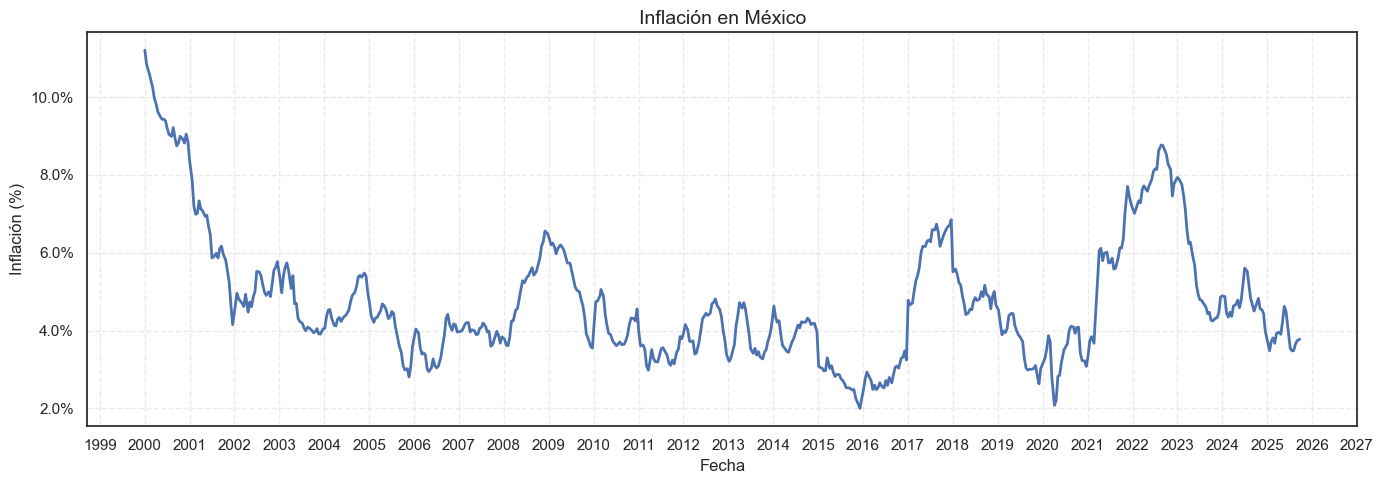
\includegraphics[width=1\textwidth]{imagenes_capitulo1/inflacion_grafico_2000_adelante.png}
    \caption{Comportamiento histórico de la inflación en México.}
    \label{fig:inflacion-mexico}
\end{figure}

\subsubsection{Esperanza}

\textbf{Definición:} El valor esperado de un proceso $\{X_t\}$ se define como
\[
\mu_t = \mathbb{E}[X_t] = \int_{-\infty}^{\infty} x f_{X_t}(x)\, dx,
\]
dado que la integral exista \cite{shumway2006time}.

En series temporales, $\mu_t$ puede ser constante o depender del tiempo.
Cuando la esperanza varía con $t$, esta función se interpreta como la
\textbf{tendencia} o \textbf{nivel} del proceso.

\subsubsection{Varianza}

La \textbf{varianza} de un proceso $\{X_t\}$ describe la dispersión de sus valores
alrededor de la media. Para un tiempo dado $t$, la varianza se define como:
\[
\mathrm{Var}(X_t) = \mathbb{E}[(X_t - \mu_t)^2].
\]

Si la varianza es constante, el proceso es \textbf{homocedástico}; si varía con el tiempo,
se denomina \textbf{heterocedástico}. En el contexto de la inflación, la varianza refleja
la \textbf{volatilidad} del proceso: periodos con choques externos (crisis financieras,
perturbaciones energéticas, políticas monetarias) suelen generar incrementos temporales en
la varianza aun cuando la tendencia general se mantenga.

\subsubsection{Autocovarianza}

\textbf{Definición:} La autocovarianza de un proceso $\{X_t\}$ está dada por
\[
\gamma(s,t) = \operatorname{Cov}(X_s, X_t)
= \mathbb{E}\!\left[(X_s - \mu_s)(X_t - \mu_t)\right],
\]
para todo par de instantes $s$ y $t$ \cite{shumway2006time}.

Esta función cuantifica la dependencia lineal entre dos observaciones en distintos tiempos.
Valores altos indican que la serie mantiene memoria a través del tiempo, mientras que valores
cercanos a cero reflejan débil dependencia lineal.

Cabe notar que $\gamma(s,t)=0$ implica ausencia de relación lineal, pero no excluye la
posibilidad de dependencias no lineales.

\subsubsection{Autocorrelación}

La \textbf{función de autocorrelación} (ACF) se define como
\[
\rho(s,t) = \frac{\gamma(s,t)}
{\sqrt{\gamma(s,s)\,\gamma(t,t)}}.
\]

La autocorrelación es simplemente la autocovarianza normalizada, acotada entre $-1$ y $1$,
y permite comparar dependencias temporales entre series con distintas escalas
\cite{shumway2006time}.

La Figura \ref{fig:acf-inflacion} muestra la ACF de la inflación mexicana, donde se observa
una fuerte persistencia en los primeros rezagos, justificando el uso de modelos capaces de
capturar dependencias temporales, tales como RNN, LSTM y arquitecturas basadas en atención.

\begin{figure}[H]
    \centering
    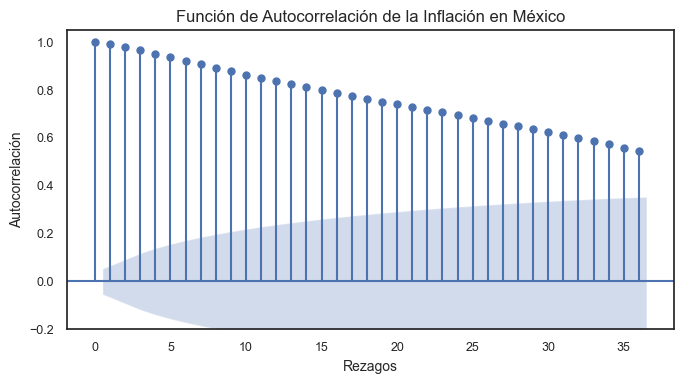
\includegraphics[width=0.85\textwidth]{imagenes_capitulo1/funcion_auto_correlacion_mexico.png}
    \caption{Función de autocorrelación (ACF) de la inflación en México.}
    \label{fig:acf-inflacion}
\end{figure}

\subsubsection{Estacionariedad}
\label{sec:Estacionaridad}

Una serie temporal es \textbf{débilmente estacionaria} si satisface tres condiciones
fundamentales \cite{shumway2006time}:
\begin{enumerate}
    \item Su media $\mu_t$ es constante en el tiempo.
    \item Su varianza $\mathrm{Var}(X_t)$ es constante y finita.
    \item Su función de autocovarianza depende únicamente del desfase $h = |t-s|$, es decir,
    \[
        \gamma(s,t) = \gamma(h).
    \]
\end{enumerate}

En la práctica, muchas series económicas —incluida la inflación— violan estas propiedades
debido a tendencias, ciclos prolongados o cambios estructurales. Por ello, antes de modelarlas
es común aplicar transformaciones que eliminen estos componentes no estacionarios y revelen
la estructura dinámica subyacente.

Una forma clásica de modelar la no estacionariedad es:
\[
X_t = \mu_t + Y_t,
\]
donde $\mu_t$ representa la tendencia de largo plazo y $Y_t$ es un proceso estacionario. La
presencia de $\mu_t$ oculta patrones de corto plazo, por lo que es deseable estimar y remover
la tendencia como parte del análisis exploratorio.

\paragraph{Diferenciación}
Una alternativa práctica consiste en aplicar la diferencia temporal:
\[
X_t - X_{t-1} \approx (Y_t - Y_{t-1}) + \delta + w_t,
\]
lo que suele producir una señal más cercana a la estacionariedad sin necesidad de especificar
paramétricamente la forma de $\mu_t$ \cite{hyndman2021forecasting}.

\begin{figure}[H]
    \centering
    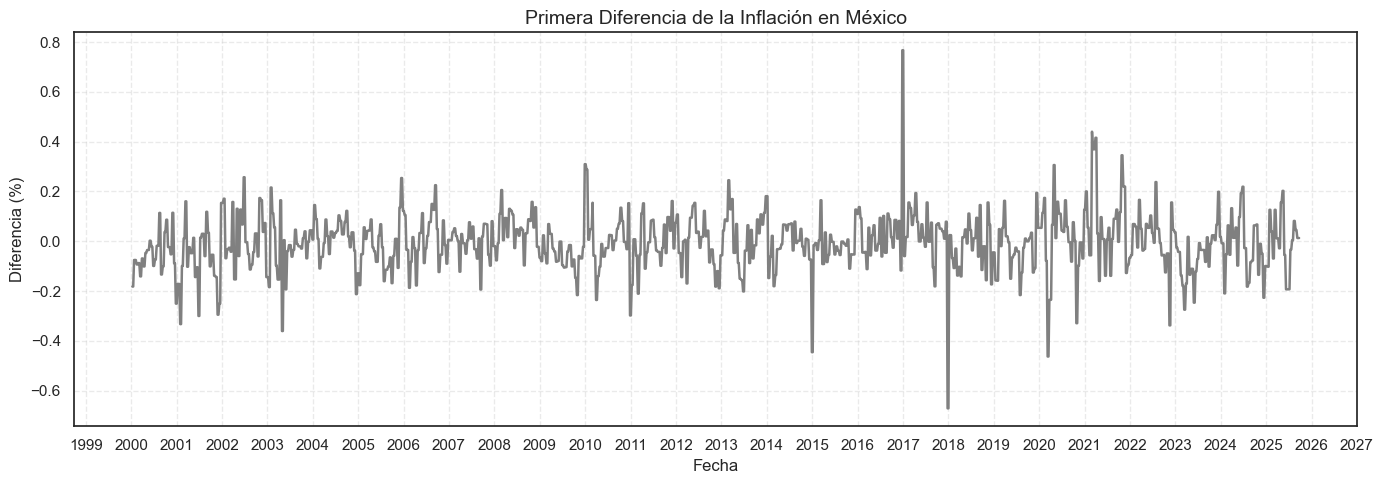
\includegraphics[width=1\textwidth]{imagenes_capitulo1/Primera_diff_inflacion_mexico_2000_onward_foward.png}
    \caption{Primera diferencia de la inflación mensual en México, utilizada para inducir estacionariedad.}
    \label{fig:diff-1-inflacion}
\end{figure}

\newpage

\subsubsection{Descomposición mediante el filtro de Hodrick--Prescott}
El filtro de Hodrick-Prescott (HP), introducido por \cite{hodrick1997postwar}, permite separar
una serie temporal en dos componentes:

\[
X_t = \tau_t + c_t,
\]

donde $\tau_t$ es una tendencia suavizada y $c_t$ representa el componente cíclico o residual,
más cercano a un proceso estacionario. Esta descomposición es especialmente útil en el caso de
la inflación, donde las variaciones de largo plazo pueden ocultar la estructura dinámica relevante.

La tendencia se obtiene como la solución del problema de optimización

\[
\min_{\{\tau_t\}_{t=1}^{T}}
\left\{
\sum_{t=1}^{T}(X_t-\tau_t)^2
+\lambda\sum_{t=2}^{T-1}
\left[(\tau_{t+1}-\tau_t)-(\tau_t-\tau_{t-1})\right]^2
\right\}.
\]

El primer término evita que la tendencia se aleje excesivamente de la serie observada, mientras que el segundo penaliza cambios abruptos en su pendiente. El parámetro $\lambda$ controla el balance entre ambas partes. Siguiendo la regla de ajuste por frecuencia propuesta por \cite{ravn2002adjusting}, se parte de $\lambda=1600$ para datos trimestrales y se utiliza

\[
\lambda_f=1600\left(\frac{f}{4}\right)^4,
\]

donde $f$ es el número de observaciones por año. Para la frecuencia semanal empleada en esta investigación, $f=52$ y, por tanto, $\lambda=45\,697\,600$.

El filtro HP es bilateral: la estimación de la tendencia cercana al final de una muestra es sensible a observaciones posteriores. Para evitar fuga de información, en cada ventana de validación el filtro se ajusta nuevamente y recibe únicamente los datos anteriores o iguales a la fecha de corte. En consecuencia, ninguna observación del horizonte evaluado participa en la descomposición utilizada para entrenar los modelos. Esta política no elimina el conocido sesgo de extremo, pero impide que el pronóstico utilice información futura de forma directa o indirecta.

Una vez obtenidos los componentes, cada arquitectura entrena dos instancias independientes:

\[
\widehat{\tau}_{t+1:t+h}=f_{\tau}(\tau_{1:t}),
\qquad
\widehat{c}_{t+1:t+h}=f_{c}(c_{1:t}),
\]

y el pronóstico final se reconstruye mediante

\[
\widehat{X}_{t+k}=\widehat{\tau}_{t+k}+\widehat{c}_{t+k},
\qquad k=1,\ldots,h.
\]

Las transformaciones descritas en la siguiente subsección se aplican exclusivamente a $\tau_t$. El ciclo se conserva en su escala estructural y únicamente se normaliza con parámetros calculados en el conjunto de entrenamiento.

La Figura~\ref{fig:hp-inflacion} muestra la inflación observada, la tendencia HP y el
componente cíclico resultante.

\begin{figure}[H]
    \centering
    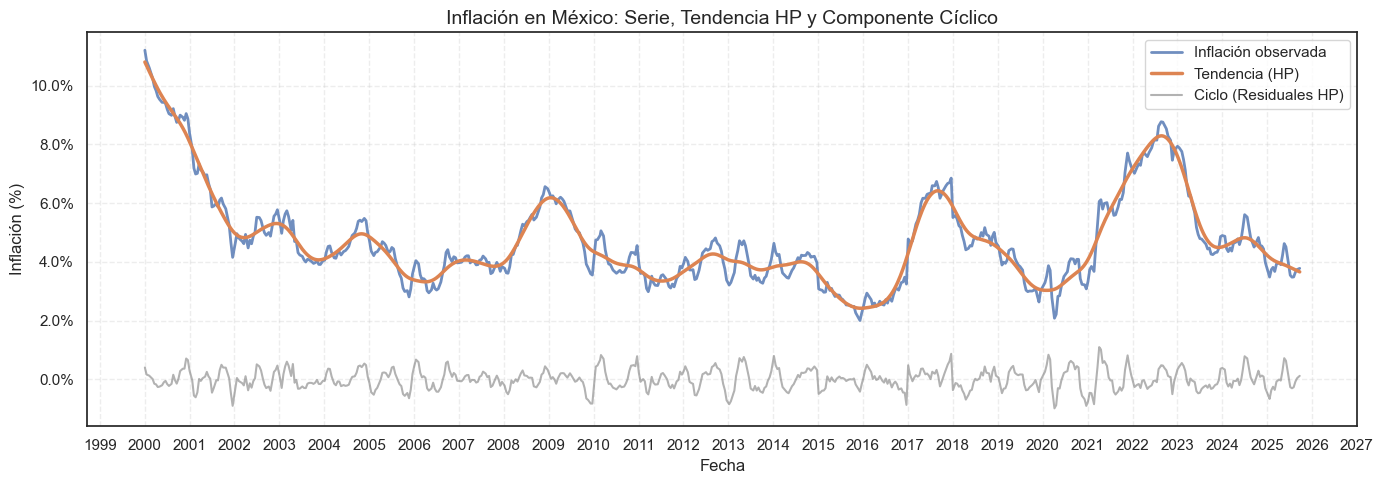
\includegraphics[width=0.95\textwidth]{imagenes_capitulo1/inflacion_en_mexico_serie_tendencia_hp_cyclic_component_KHE.png}
    \caption{Inflación mensual en México: serie original, tendencia estimada mediante el filtro HP y componente cíclico.}
    \label{fig:hp-inflacion}
\end{figure}

\subsubsection{Transformaciones aplicadas}

Para inducir estacionariedad y mejorar el desempeño de los modelos predictivos, el framework
implementado en este trabajo permite aplicar diversas transformaciones a la serie original.
Estas transformaciones estabilizan la varianza, eliminan tendencias o resaltan cambios relativos.
Las opciones disponibles incluyen:

\paragraph{1. Diferencia simple (diff)}
\[
\nabla x_t = x_t - x_{t-1}.
\]
Elimina tendencias lineales y resalta variaciones de corto plazo \cite{hyndman2021forecasting}.

\paragraph{2. Diferencia del logaritmo amortiguado (diff\_logp1)}
\[
\nabla \log(1 + x_t) = \log(1 + x_t) - \log(1 + x_{t-1}).
\]
Reduce el impacto de valores extremos y convierte cambios absolutos en relativos.

\paragraph{3. Cambio porcentual (pct)}
\[
\frac{x_t - x_{t-1}}{x_{t-1}}.
\]
Captura variaciones proporcionales e induce homocedasticidad en diversas series económicas.

\paragraph{4. Transformación logarítmica amortiguada (logp1)}
\[
\log(1+x_t).
\]
Suaviza la serie y estabiliza la varianza.

\paragraph{5. Segunda diferencia (diff2)}
\[
\nabla^2 x_t = (x_t - x_{t-1}) - (x_{t-1} - x_{t-2}).
\]
Elimina tendencias de orden superior o estructuras suavemente crecientes.

Estas transformaciones fueron implementadas de manera parametrizable dentro del sistema, lo que
permite seleccionar la opción más adecuada para cada serie. No obstante, es importante evitar una
``sobre-estacionarización'', ya que transformar en exceso la serie puede eliminar información
relevante para el proceso generador \cite{hyndman2021forecasting}.

\subsection{Embedding}

Un \textbf{embedding} es una representación vectorial en un espacio continuo de dimensión
reducida, utilizada para transformar elementos discretos, como categorías, identificadores
o índices temporales en vectores de números reales. Su propósito es capturar
relaciones latentes entre los elementos de manera que aquellos más similares queden
cercanos entre sí dentro del espacio geométrico de representación
\cite{mikolov2013efficient}.

Formalmente, un embedding es una función
\[
f: \mathcal{C} \rightarrow \mathbb{R}^d,
\]
donde $\mathcal{C}$ es un conjunto discreto (por ejemplo, meses, días de la semana,
palabras, imágenes o identificadores de series), y $d$ es la dimensión del espacio
vectorial continuo.

\begin{figure}[H]
    \centering
    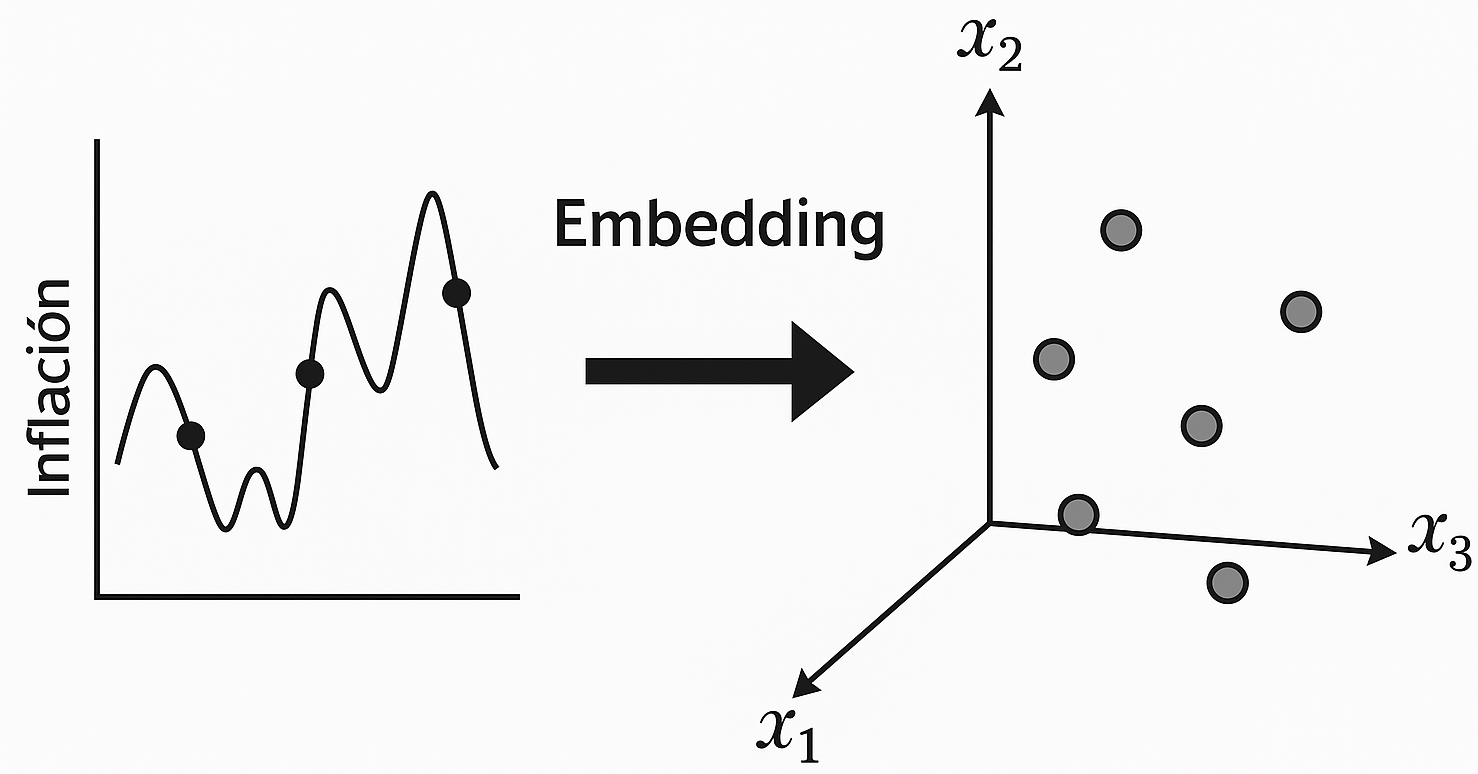
\includegraphics[width=0.9\textwidth]{imagenes_capitulo1/embedding_inflacion_3d.png}
    \caption{Representación conceptual del embedding: cada observación de la serie de inflación se proyecta a un espacio vectorial tridimensional.}
    \label{fig:embedding_3d}
\end{figure}

En el contexto de series temporales, los embeddings permiten representar atributos
temporales (como el índice de tiempo, el mes del año o identificadores de series) en un
espacio donde los modelos neuronales pueden operar mediante álgebra lineal. Esta
representación densa es fundamental en arquitecturas modernas como LSTM, Transformer y
D\textsuperscript{3}VAE, las cuales dependen de embeddings para capturar dependencias
temporales y relaciones entre series individuales.

\subsection{Fundamentos probabilísticos}

Muchos de los modelos empleados en este trabajo, en particular DeepAR y
D\textsuperscript{3}VAE, se formulan explícitamente en términos probabilísticos. Estos
métodos estiman distribuciones de probabilidad condicionales, optimizan funciones de
log-verosimilitud y utilizan divergencias entre distribuciones para regularizar espacios
latentes o medir discrepancias. Con este fin, se presentan a continuación algunos
conceptos fundamentales necesarios para comprender estos modelos
\cite{bishop2006pattern, murphy2023pml}.

\subsubsection{Operaciones básicas sobre distribuciones de probabilidad}

Sea \(p(x)\) una función de densidad de probabilidad (PDF) definida sobre una variable
aleatoria continua \(x\). Algunas operaciones fundamentales en modelos probabilísticos son:

\begin{itemize}
    \item \textbf{Logaritmo de la densidad}:
    \[
        \log p(x).
    \]
    El uso del logaritmo facilita el cálculo numérico y es esencial en el aprendizaje por
    máxima verosimilitud, donde se optimiza la log-verosimilitud en lugar de la
    verosimilitud directa \cite{bishop2006pattern}.

    \item \textbf{Gradiente del logaritmo}:
    \[
        \nabla_x \log p(x) = \frac{\nabla_x p(x)}{p(x)}.
    \]
    Esta cantidad, conocida como \textit{score function}, describe la dirección de máximo
    incremento relativo de la densidad. Es útil en métodos de optimización y en técnicas de
    estimación basadas en gradientes \cite{murphy2023pml}.
\end{itemize}

\subsubsection{Logaritmo de una distribución normal}

Si \(x \sim \mathcal{N}(\mu,\sigma^2)\), su densidad es:
\[
p(x) = \frac{1}{\sqrt{2\pi\sigma^2}}
\exp\left(-\frac{(x-\mu)^2}{2\sigma^2}\right).
\]

El logaritmo de la densidad se obtiene aplicando logaritmo natural:
\[
\log p(x)
= -\frac{(x-\mu)^2}{2\sigma^2}
  -\frac{1}{2}\log(2\pi\sigma^2),
\]
lo que corresponde a una parábola invertida en \(x\), acompañada de un término constante.

El gradiente de la log-densidad es:
\[
\nabla_x \log p(x) = -\frac{x-\mu}{\sigma^2}.
\]

Esta expresión indica que la fuerza con la cual la densidad ``empuja'' a \(x\) hacia la media
es proporcional a la distancia \(x-\mu\), escalada por el inverso de la varianza. Este
comportamiento es fundamental en modelos latentes gaussianos y en la inferencia variacional
\cite{kingma2014vae}.

\subsubsection{Divergencia de Kullback--Leibler}

La divergencia de Kullback--Leibler (\( \mathcal{D}_{KL} \)) mide la discrepancia entre dos
distribuciones de probabilidad \(p(x)\) y \(q(x)\):
\[
\mathcal{D}_{KL}(p||q) =
\int p(x)\,\log\left(\frac{p(x)}{q(x)}\right) \, dx.
\]

Sus propiedades principales son \cite{kullback1951information}:
\begin{itemize}
    \item \textbf{No negatividad}: \( \mathcal{D}_{KL}(p||q) \ge 0\).
    \item \textbf{Identidad}: \( \mathcal{D}_{KL}(p||q)=0\) si y sólo si \(p=q\) casi siempre.
    \item \textbf{Asimetría}: \( \mathcal{D}_{KL}(p||q)\neq\mathcal{D}_{KL}(q||p)\).
\end{itemize}

En modelos generativos como las VAEs, la divergencia KL actúa como un término de
regularización que controla cuán cerca se mantiene la distribución aproximada del posterior
respecto a un \textit{prior} elegido, jugando un papel fundamental en la calidad del espacio
latente \cite{kingma2014vae}.

Estas herramientas probabilísticas serán utilizadas posteriormente al describir modelos
como DeepAR y D\textsuperscript{3}VAE, los cuales formulan el problema de pronóstico como
la estimación de una distribución condicional y emplean funciones de pérdida basadas en
log-verosimilitud o divergencias entre distribuciones.

\subsection{Transformación Discreta de Fourier (DFT)}

La Transformación Discreta de Fourier (DFT) es una herramienta matemática que permite
descomponer una serie temporal como una combinación de componentes senoidales de distintas
frecuencias. Su propósito es representar la señal en el dominio de la frecuencia, lo cual
facilita la identificación de patrones cíclicos, estacionalidades u oscilaciones dominantes
\cite{roberts2019spectral}.

Dada una secuencia de observaciones
\[
x_0, x_1, \dots, x_{N-1},
\]
la DFT se define como:

\begin{equation}
    X_k = \sum_{n=0}^{N-1} x_n\, e^{-2\pi i \frac{kn}{N}},
    \qquad k = 0, 1, \dots, N-1.
\end{equation}

Aquí, \(X_k\) representa la amplitud y fase asociadas a la frecuencia \(k\). Esta representación
permite reconstruir la señal original mediante la transformada inversa:

\begin{equation}
    x_n = \frac{1}{N} \sum_{k=0}^{N-1} X_k\, e^{2\pi i \frac{kn}{N}}.
\end{equation}

En el presente trabajo, la DFT se aplica a la serie inflacionaria con el propósito de identificar
las frecuencias de mayor energía y utilizarlas para construir variables exógenas senoidales. A
partir de las \(k\) frecuencias dominantes se generan funciones seno y coseno normalizadas que
capturan estacionalidades explícitas. Estas variables son integradas posteriormente en modelos
como XGBoost, LSTM, RNN, DeepAR y Transformer.

Este procedimiento aporta información periódica sin requerir que los modelos aprendan todas las
estacionalidades de manera implícita, mejorando su capacidad para capturar patrones recurrentes
en escalas largas y medianas.

\subsection{Fundamentos estadísticos del aprendizaje}

El presente capítulo tiene como propósito establecer los principios matemáticos y estadísticos que sustentan el aprendizaje automático aplicado en esta investigación. Estos fundamentos permiten entender los mecanismos detrás del proceso de modelado, la naturaleza de los errores de predicción y las métricas utilizadas para evaluar el desempeño de los algoritmos.

\subsubsection{Formulación general del problema de aprendizaje}
Sea un conjunto de observaciones $\{(x_i, y_i)\}_{i=1}^{n}$, donde cada $x_i \in \mathbb{R}^p$ representa un vector de predictores o variables explicativas y $y_i \in \mathbb{R}$ la variable de respuesta.
Se asume la existencia de una función desconocida $f$ que relaciona ambas cantidades:
\[
Y = f(X) + \epsilon,
\]
donde $\epsilon$ representa un término de error aleatorio con media cero, $\mathbb{E}[\epsilon] = 0$, y varianza constante $\text{Var}(\epsilon) = \sigma^2$.
El objetivo del aprendizaje estadístico consiste en estimar una función $\hat{f}$ que aproxime de la mejor manera posible a $f$, minimizando la discrepancia entre las predicciones $\hat{y}_i = \hat{f}(x_i)$ y los valores reales $y_i$.

Este proceso puede entenderse como una búsqueda en el espacio de funciones posibles $\mathcal{F}$, de modo que:
\[
\hat{f} = \arg\min_{f \in \mathcal{F}} \mathbb{E}\big[(Y - f(X))^2\big].
\]
En la práctica, la esperanza no se conoce, por lo que se utiliza una versión empírica basada en el conjunto de entrenamiento disponible.

\subsubsection{Error reducible e irreducible}
El error esperado de predicción en un punto $x_0$ se descompone de la siguiente forma:
\[
\mathbb{E}\big[(Y - \hat{f}(X))^2\big] =
\underbrace{\mathbb{E}\big[(f(X) - \hat{f}(X))^2\big]}_{\text{Error reducible}}
+
\underbrace{\text{Var}(\epsilon)}_{\text{Error irreducible}}.
\]
El \textit{error reducible} depende de la capacidad del modelo para aproximar correctamente la función $f$.
Mediante una mejor arquitectura, mayor cantidad de datos o un ajuste adecuado de hiperparámetros, este término puede disminuirse.
Por otro lado, el \textit{error irreducible} corresponde a la variabilidad inherente del proceso generador de los datos; es decir, al ruido que no puede ser explicado por ninguna función de $X$.
Este componente establece un límite inferior en la exactitud de cualquier modelo predictivo. \cite{texbook_ISLR}

\subsubsection{Descomposición sesgo–varianza}
Para un punto nuevo $x_0$, el error cuadrático medio esperado puede descomponerse como:
\[
\mathbb{E}\big[(y_0 - \hat{f}(x_0))^2\big]
=
\text{Var}\big(\hat{f}(x_0)\big)
+
\Big[\text{Bias}\big(\hat{f}(x_0)\big)\Big]^2
+
\text{Var}(\epsilon).
\]
El segundo término mide el \textit{sesgo} (bias), es decir, la diferencia sistemática entre el valor esperado de la predicción y el valor real.
El primero representa la \textit{varianza}, que indica qué tanto cambia la predicción ante distintos conjuntos de entrenamiento.

Modelos muy flexibles (como las redes neuronales profundas) suelen tener bajo sesgo pero alta varianza, mientras que modelos rígidos (como las regresiones lineales) presentan el comportamiento opuesto.
El objetivo del aprendizaje estadístico es encontrar un punto de equilibrio donde tanto el sesgo como la varianza sean bajos, logrando así una buena generalización en datos no observados. \cite{texbook_ISLR}

\subsubsection{Métricas de evaluación}
La evaluación de un modelo requiere cuantificar qué tan cercanas son sus predicciones a los valores reales.
Entre las métricas más comunes utilizadas en esta tesis se encuentran:

\[
\textbf{MAE} = \frac{1}{n} \sum_{i=1}^{n} |y_i - \hat{y}_i|,
\qquad
\textbf{MSE} = \frac{1}{n} \sum_{i=1}^{n} (y_i - \hat{y}_i)^2,
\]
\[
\textbf{RMSE} = \sqrt{\frac{1}{n} \sum_{i=1}^{n} (y_i - \hat{y}_i)^2},
\qquad
\textbf{MAPE} = \frac{100}{n} \sum_{i=1}^{n} \frac{|y_i - \hat{y}_i|}{|y_i|}.
\]
En el presente estudio se adopta el \textbf{Error Absoluto Medio (MAE)} como métrica principal de comparación, debido a su robustez frente a valores atípicos y su interpretación directa en unidades de inflación.
Las demás métricas se incluyen con fines complementarios y de contraste en el análisis de resultados.

\subsubsection{Error de predicción y evaluación fuera de muestra}
Durante el entrenamiento, el modelo se ajusta para minimizar el error sobre el conjunto de entrenamiento.
Sin embargo, el interés real radica en medir su desempeño en observaciones no vistas previamente.
Sea $(x_0, y_0)$ una nueva observación, la capacidad predictiva se evalúa a través del error:
\[
e_0 = y_0 - \hat{f}(x_0),
\]
y su valor absoluto medio a lo largo de todo el conjunto de prueba.
Un modelo con bajo error en entrenamiento pero alto error en prueba se considera sobreajustado, mientras que un modelo con errores altos en ambos conjuntos probablemente sea insuficientemente flexible.

\subsubsection{Linealidad y mínimos cuadrados}
En el contexto de predicción de series temporales, un modelo puede perder utilidad si sus predicciones son excesivamente lineales.
Para evaluar este fenómeno, se ajusta la recta que mejor aproxima las predicciones mediante el método de mínimos cuadrados lineales, resolviendo:
\[
\min_{m,b} \sum_{t} \big(\hat{y}_t - (m t + b)\big)^2,
\]
donde $m$ es la pendiente y $b$ la ordenada al origen.
El ajuste se realiza a través del sistema matricial:
\[
A =
\begin{bmatrix}
0 & 1 \\
1 & 1 \\
2 & 1 \\
\vdots & \vdots \\
n-1 & 1
\end{bmatrix},
\qquad
A^\top A
\begin{bmatrix}
m \\ b
\end{bmatrix}
=
A^\top \hat{y}.
\]
El error cuadrático medio entre la línea ajustada y las predicciones permite cuantificar el grado de linealidad:
\[
\text{RMSE}_{\text{lin}} =
\sqrt{\frac{1}{n} \sum_t (\hat{y}_t - (m t + b))^2}.
\]
Si este valor es muy bajo, se considera que el modelo está generando pronósticos lineales y, por tanto, poco informativos respecto a una regresión o promedio histórico.
Este criterio se implementa en los experimentos como un filtro adicional para evitar configuraciones triviales.

\begin{figure}[!h]
\centering
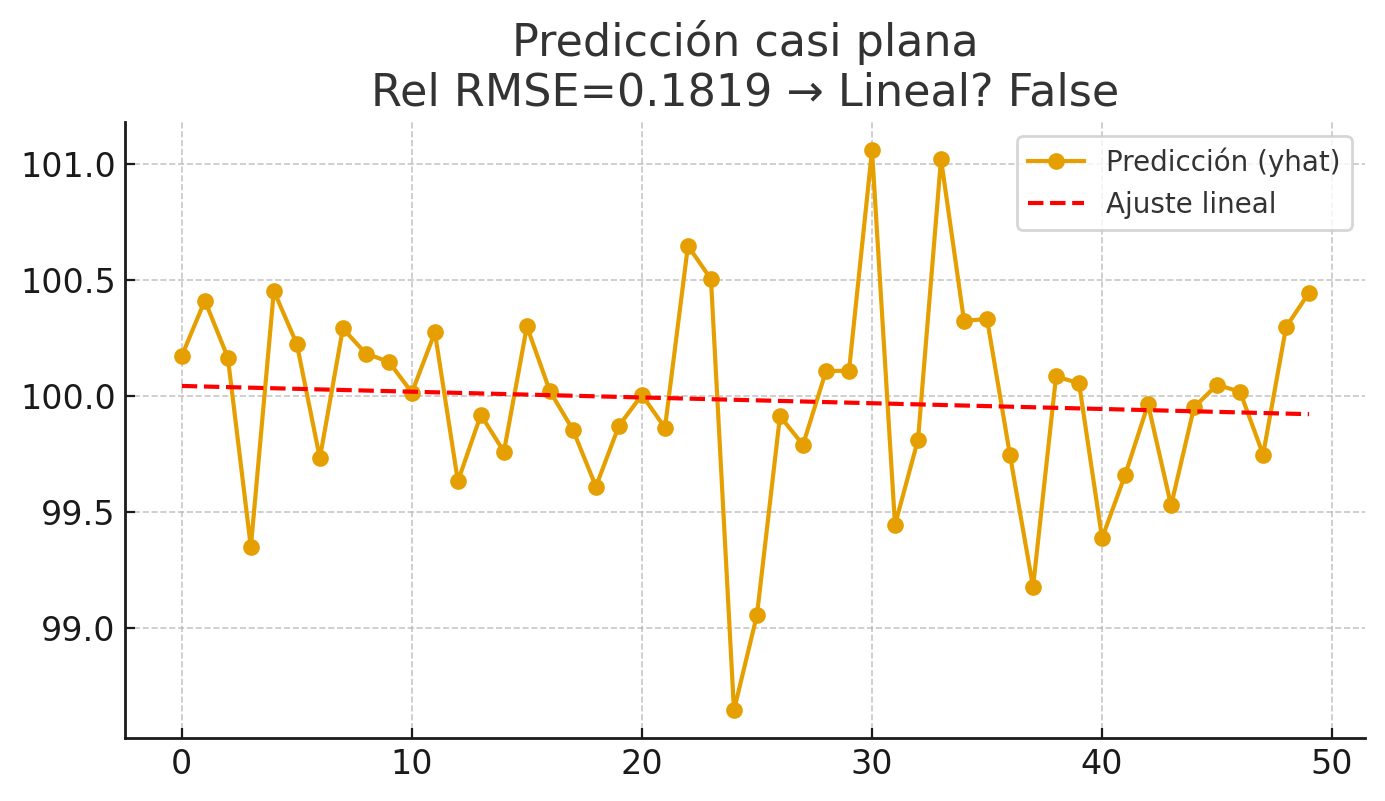
\includegraphics[width=0.85\textwidth]{penalizacion.png}
\caption{Detección de Pronósticos Lineales}
\label{fig:pen_regresion_forecasted}
\end{figure}

\newpage

\section{Espectro de Modelos de Pronóstico de Inflación: De Enfoques Simples a Arquitecturas Avanzadas de Aprendizaje Profundo}

\subsection{Naive}
Esto método es el más simple de todos, consiste en tomar el ultimo valor conocido en una serie temporal, como la predicción para el valor futuro $y_{t+1}$
\begin{equation}
    \hat{y}_{t+1} = y_{t}.
\end{equation}

\subsection{Promedio}
Otro método simple es usar el promedio de todos los valores conocidos en la serie temporal hasta el momento $t$, y tomar este valor como la predicción futura. Es decir,
\begin{equation}
    \hat{y}_{t+1} = \frac{1}{t}\sum_{i=1}^x y_i.
\end{equation}

\subsection{Suavizado Exponencial Simple}
Este modelo propone asignarle un peso a todos los valores de la serie temporal, de tal manera que los valores más cercanos al tiempo $t$ tendrán más peso que aquellos valores lejanos a $t$.

\begin{equation}
    \hat{y}_{t+1} = \alpha y_t+ (1-\alpha) \hat{y}_t.
\end{equation}

Si se desarrolla la parte derecha de la ecuación anterior, y se reemplaza recursiva-mente $\hat{y}_{t-1}$, se obtiene una expansión infinita ponderada de valores pasados. Por lo tanto al desarrollar se tiene lo siguiente...

\begin{align}
     \hat{y}_{t+1} &= \alpha y_t+ (1-\alpha) \hat{y}_t\\
     &= \alpha y_t + (1-\alpha)\big[ \alpha y_{t-1 } + (1-\alpha) \hat{y}_{t-1} \big]\\
     &= \alpha y_t + \alpha(1-\alpha) y_{t-1}+(1-\alpha)^2 \hat{y}_{t-1}\\
     &= \alpha y_t + \alpha(1-\alpha) y_{t-1}+(1-\alpha)^2\big[ \alpha y_{t-2} + (1-\alpha)\hat{y}_{t-2} \big]\\
     &= \alpha y_t + \alpha(1-\alpha) y_{t-1}+\alpha(1-\alpha)^2 y_{t-2}+(1-\alpha)^3\hat{y}_{t-2}\\
     &\quad \vdots \nonumber \\
     &= \sum_{i=0}^{\infty} \alpha(1-\alpha)^i y_{t-i}.
\end{align}

De acuerdo con \cite{nist-ses}, el suavizado exponencial simple no es bueno cuando los datos presentan tendencia. El coeficiente $\alpha$ simplemente no es suficiente.

\subsection{Suavizado Exponencial Doble (Holt)}

\subsubsection{Nivel}
El nivel, no es más que el valor esperado. Este se puede interpretar como

\subsubsection{Tendencia o Pendiente}
Es una operación que hemos visto a lo largo de toda nuestra vida, esta se calcula como
\begin{equation}
    m = \frac{\triangle y}{\triangle t}.
\end{equation}

Donde $\triangle y$ es la diferencia de los valores observados $y$, y $\triangle t$ es la diferencia de los momentos $t$ de acuerdo con los valores observados de $y$.

Como su nombre lo dice, se aplica suavizado exponencial a dos componentes, al nivel \(\ell_t\) y la tendencia \(b_t\), los cuales se definen a continuación.
\begin{align}
    \ell_t &= \alpha y_t + (1 - \alpha)(\ell_{t-1} + b_{t-1}) \\
    b_t &= \beta(\ell_t - \ell_{t-1}) + (1 - \beta) b_{t-1}.
\end{align}

Por lo tanto, para valores futuros se tiene...
\[
\hat{y}_{t+1} = \ell_t + b_t
\]
Note que $\ell_t$ es lo mismo que la ecuación 5, con la diferencia de que se multiplica la constante $(1-\alpha)$ por la suma del valor esperado  pasado $\ell_{t-1}$ más la tendencia pasada $b_{t-1}$.

Vamos a desarrollar \(\ell_t\) y \(b_t\) recursivamente para entender cómo todo depende de las observaciones pasadas \(y_t, y_{t-1}, \dots\)

\begin{align}
    \ell_t &= \alpha y_t + (1 - \alpha)(\ell_{t-1} + b_{t-1}) \\
           &= \alpha y_t + (1 - \alpha)\left[ \alpha y_{t-1} + (1 - \alpha)(\ell_{t-2} + b_{t-2}) + b_{t-1} \right] \\
           &= \alpha y_t + \alpha(1 - \alpha) y_{t-1} + (1 - \alpha)^2 (\ell_{t-2} + b_{t-2}) + (1 - \alpha) b_{t-1}.
\end{align}

De manera similar, para la tendencia:

\begin{align}
    b_t &= \beta(\ell_t - \ell_{t-1}) + (1 - \beta) b_{t-1} \\
        &= \beta(\ell_t - \ell_{t-1}) + (1 - \beta)\left[ \beta(\ell_{t-1} - \ell_{t-2}) + (1 - \beta) b_{t-2} \right] \\
        &= \beta(\ell_t - \ell_{t-1}) + \beta(1 - \beta)(\ell_{t-1} - \ell_{t-2}) + (1 - \beta)^2 b_{t-2}.
\end{align}

Esto significa que tanto el nivel como la tendencia se construyen como combinaciones suavizadas de observaciones pasadas y de sus propios estados anteriores. Si seguimos expandiendo, veremos que ambos se expresan como una especie de media ponderada exponencial de diferencias y valores pasados, aunque más compleja que en el suavizado exponencial simple.

Por lo tanto, el pronóstico \( \hat{y}_{t+h} \) puede interpretarse como una extrapolación lineal ajustada dinámicamente:
\[
\hat{y}_{t+h} = \ell_t + h b_t
\]
donde \( \ell_t \) y \( b_t \) ya encapsulan toda la información histórica de \( y_t \).

De acuerdo con \cite{nist-des}, para definir los valores iniciales de la tendencia, se tienen las siguientes opciones.
\begin{align}
    b_1 &= y_2 - y_1\\
    b_1 &= \frac{1}{3} \big[ (y_2-y_1) + (y_3 - y_2) + (y_4-y_3)\big]\\
    b_1 &= \frac{y_n - y_1}{n-1}.
\end{align}
Mientras que el valor esperado suele ser $\ell_1=y_1$, tal como ocurre en el suavizado exponencial simple.


\subsection{Suavizado Exponencial Triple - Holt Winters}
Si la serie temporal que se esta buscando modelar presenta tendencia y estacionalidad, el suavizado exponencial doble no funcionará, mucho menos el simple. De acuerdo con \cite{grisha-triple-exp}, la idea detrás del suavizado exponencial triple es aplicar el suavizado exponencial a tres factores, los componentes estacionales $s$, el valor esperado $\ell$ y la tendencia $b$. El resultado de las siguientes ecuaciones es conocido como el método "Holt Winters", este nombre sale de sus inventores.

\subsubsection{Estación}
En el contexto de series temporales, se puede definir a una estación como la repetición de un patrón dado un cierto intervalo de pasos. Si una serie presenta estacionalidad, ya sea por la época del año, descuentos u otra variable predictora, el método de Holt Winters se vuelve en una buena opción para modelar este tipo de series.

\subsubsection{Longitud de una Estación}
La longitud de una estación es la cantidad de pasos requeridos para que una nueva estación comience. En general, para datos semanales, se puede tener una longitud de $52.14\approx52$.

\subsubsection{Componentes Estacionales}
Un componente estacional sale del valor esperado más la tendencia que se repiten al mismo tiempo en la estación. Existe un componente estacional por cada punto en una estación. Por lo que si se tiene una estacionalidad de 12 meses, entonces habrá 12 componentes estacionales. Si los datos son agrupados de forma semanal, entonces se tendrá un total de 52 componentes estacionales. \cite{grisha-triple-exp}

\subsubsection{Adición vs Multiplicación}
La tendencia en una serie temporal puede ser explicada de forma aditiva o multiplicativa, es decir, en lugar de substraer $y_{t-1}$ de $y_{t}$, se pueden dividir y obtener en su lugar el porcentaje de cambio. Por un lado puedes decir que algo ahora cuesta 30 pesos más, y por otro, que aumento el precio en un $10\%$. Esto es lo que da paso a que existan dos variantes del método de Holt Winters.

La versión aditiva se define de la siguiente manera y se usa cuando la estacionalidad tiene una variación aproximadamente constante en el tiempo.

\begin{align}
    \ell_t &= \alpha(y_t - s_{t-L}) + (1-\alpha)(\ell_{t-1}+b_{t-1})\\
    b_t &= \beta(\ell_t - \ell_{t-1})+(1-\beta)b_{t-1}\\
    s_t &= \gamma(y_t - \ell_{t-1} - b_{t-1})+(1-\gamma)s_{t-L}\\
    \hat{y}_{t+h} &= \ell_t + hb_t + s_{t+h-L(k+1)}.
\end{align}
donde $k$ es la parte entera de $\frac{h-1}{m}$, la cual asegura que las estimaciones de los indices estacionales usados para pronosticar provengan de la última estación de la muestra. Véase que la ecuación del nivel $\ell_t$ es un promedio ponderado entre el valor observado y la estacionalidad ajustada $(y_t-s_{t-L})$ y el pronostico no estacional $(\ell_{t-1}+b_{t-1})$ para el momento t. Por otro lado, la ecuación correspondiente a la tendencia $b_t$ permanece igual que en el método de Holt. Mientras que la ecuación de estacionalidad $s_t$ es el promedio ponderado entre $(y_t-\ell_{t-1}-b_{t-1})$ y el indice estacional correspondiente al periodo pasado $s_{t-L}$. \cite{hyndman2018forecasting}

Mientras que la versión multiplicativa se usa cuando la estacionalidad tiene una variación proporcional al nivel de la serie. \cite{hyndman2018forecasting}.

\begin{align}
    l_t &= \alpha( \frac{y_t}{s_{t-L}}) + (1-\alpha)(l_{t-1}+b_{t-1})\\
    b_t &= \beta^*(l_t - l_{t-1}) + (1-\beta^*)b_{t-1}\\
    s_t &= \gamma \frac{y_t}{l_t}+(1-\gamma)s_{t-L}\\
    \hat{y}_{t+h} &= (l_t + hb_t )s_{t+h-L(k+1)}.
\end{align}

Donde $\alpha, \beta^*, \gamma$ son parámetros de suavizado $(0<\alpha, \beta^*, \gamma<1)$ y $m$ es la longitud del período  estacional.

Para poder usar el método de Holt Winters es necesario poseer por lo menos una estacionalidad completa para determinar los valores iniciales de los indices de estacionalidad $s_{t-L}$. Una estación completa de observaciones consiste de $L$ periodos. Y se desea estimar la tendencia de un periodo a otro. Para lograr esto, es necesario usar dos estaciones completas, es decir, $2L$ periodos/observaciones.

Los valorees iniciales para la tendencia se obtienen a partir de la siguiente formula
\begin{equation}
b=\frac{1}{L} \bigg( \frac{y_{L+1}-y_1}{L} + \frac{y_{L+2}-y_2}{L} + \dots + \frac{y_{L+L}-y_L}{L} \bigg).
\end{equation}

Mientras que los valores iniciales de los índices estacionales se calculan a partir de la media de cada estación y de la media global de las primeras $N$ estaciones completas. Para el modelo aditivo, los índices estacionales se definen como:

\begin{equation}
s_i = \frac{1}{N} \sum_{j=1}^{N} (y_{L(j-1)+i} - \bar{y}_j), \quad i = 1,2,\dots,L.
\end{equation}

donde $\bar{y}_j$ representa la media de la $j$-ésima estación, y $L$ es la longitud de la estación (por ejemplo, 12 para datos mensuales o 52 para datos semanales).
En el caso del modelo multiplicativo, los índices estacionales se obtienen dividiendo cada observación entre la media de su estación:

\begin{equation}
s_i = \frac{1}{N} \sum_{j=1}^{N} \frac{y_{L(j-1)+i}}{\bar{y}_j}, \quad i = 1,2,\dots,L.
\end{equation}

De esta manera, los valores iniciales de tendencia, nivel y estacionalidad permiten al método de Holt-Winters comenzar el proceso iterativo de actualización y pronóstico.
En cada paso, los parámetros se ajustan mediante las ecuaciones de suavizado exponencial, dando más peso a las observaciones recientes, lo que confiere al modelo una respuesta adaptativa ante cambios estructurales en la serie temporal.

\section*{Árboles de Decisión}
Los \textit{Árboles de Decisión} son aplicados a problemas de regresion y clasificación. Y hay una gran variedad de algoritmos basados en árboles. Éstos implican la segmentación del espacio predictor en un número de regiones simples (rectangulares). Para hacer una predicción en una observación $x_0$, toman el promedio o la moda de la variable de respuesta de la región para la cual la observación $x_0$ pertenece. Los árboles de decisión son simples y fáciles de interpretar. Algoritmos como \textit{bagging, random forests, boosting} y \textit{árboles de regresion aditivos bayesianos} producen múltiples árboles, los cuales se combinan para crear una predicción final. Combinar una gran cantidad de árboles mejoran la capacidad predictora de estos algoritmos, pero se pierde en interpretabilidad.

\begin{figure}[!h]
    \centering
    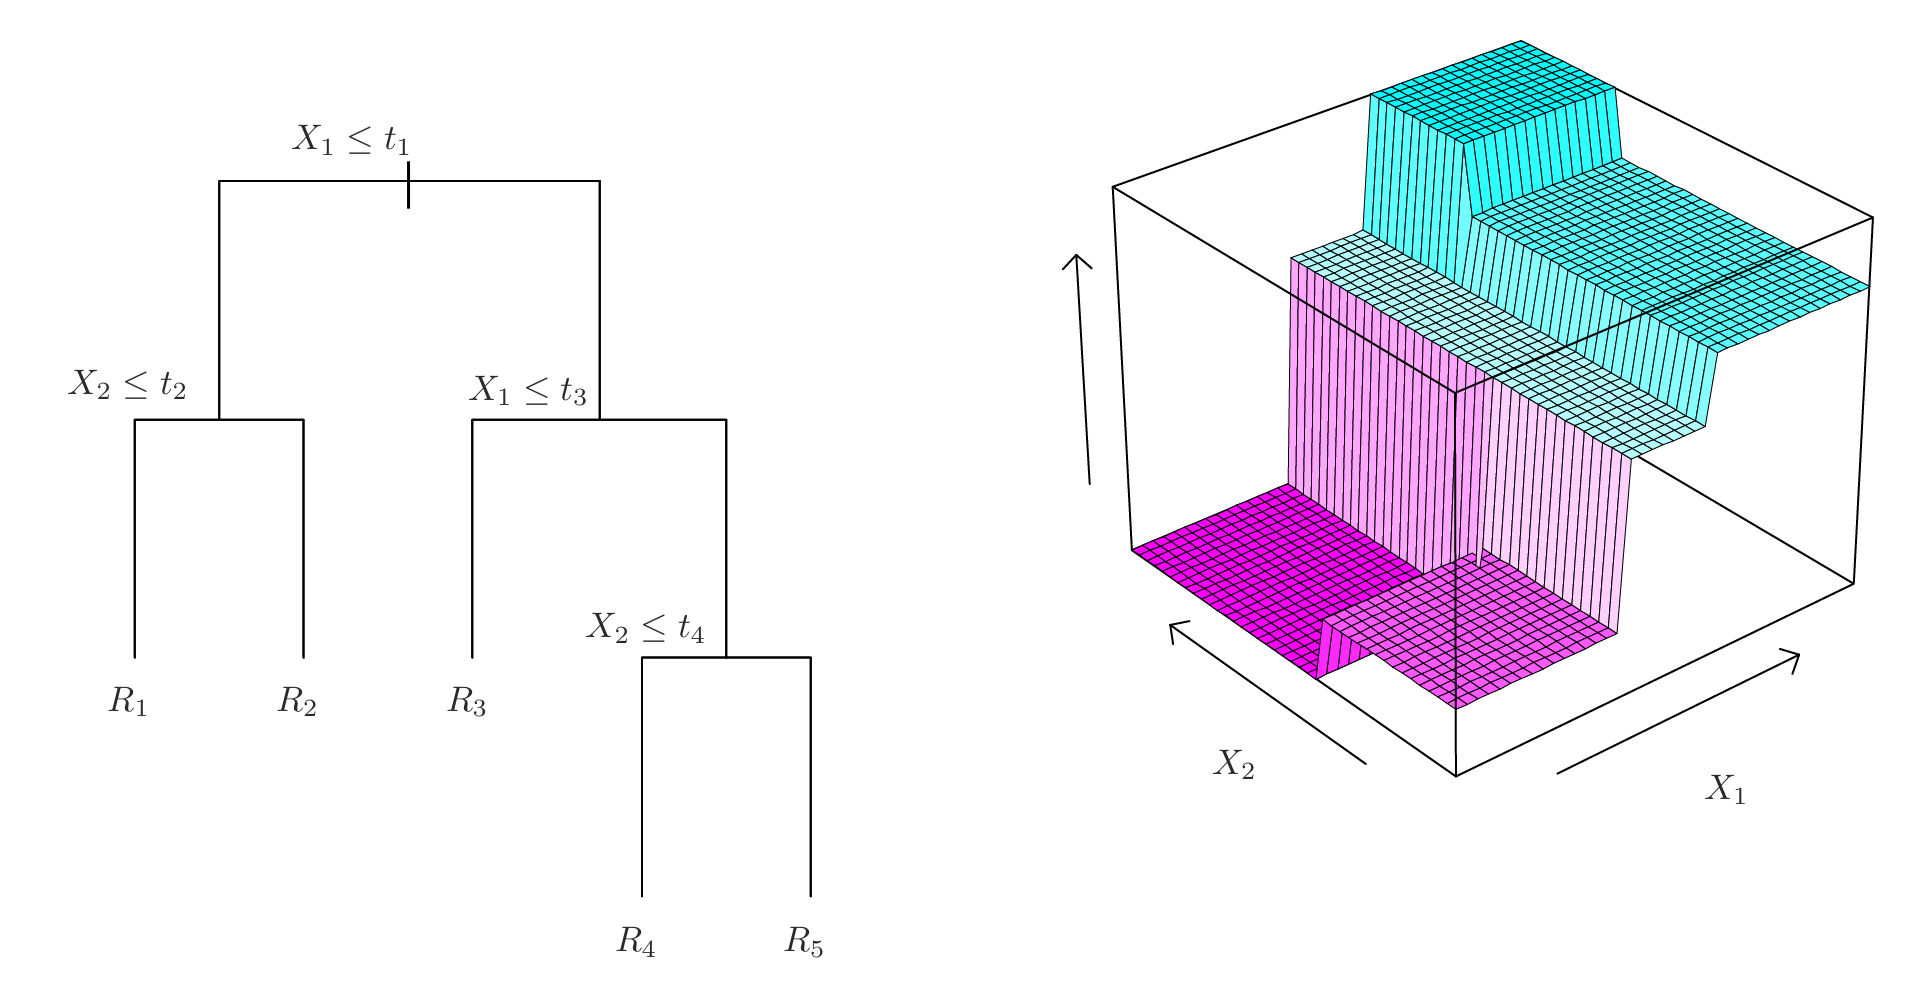
\includegraphics[width=0.8\textwidth]{arquitecturas/arboles_decision.png}
    \caption{Ejemplo de un árbol de decisión proveniente de \cite{texbook_ISLR}.}
    \label{fig:xgboost-tree-surface}
    %\source{\cite{texbook_ISLR}}
\end{figure}


\subsection{XGBoost}
XGBoost es un ensamble de $K$ arboles, donde cada uno contribuye de manera aditiva a la predicción final con una estructura como la que se muestra en la figura \ref{fig:xgboost-tree-surface}, y la predicción se obtiene como:
\begin{equation}
    \hat{y}_i = \phi(x_i)=\sum_{k=1}^k f_k(x_i),\,\, f_k\in \mathcal{F}.
\end{equation}
El espacio de funciones $\mathcal{F}$ está definido como:
\begin{equation}
\mathcal{F} = {f(x) = w_{q(x)}},
\end{equation}
Donde $q:\mathbb{R}^m\to T$ es una función que asigna una observación \textbf{x} a una de las $T$ hojas del árbol, mientras que  $w\in \mathbb{R}^T$ es el vector de pesos asignados a cada hoja. Por lo tanto, cada función $f_k$ representa un árbol con una estructura $q$ y valores de predicción $w$ en sus hojas. \cite{chen2016xgboost}

\subsubsection{Aprendizaje de Árboles}
Para aprender el conjunto de funciones usadas en el modelo, se minimiza la función objetivo regularizado...
\begin{equation}
\mathcal{L}(\phi) = \sum_i \ell(y_i, \hat{y}i) + \sum_k \Omega(f_k),
\end{equation}
donde  $\ell$ es una función de pérdida convexa diferenciable, la cual mide la diferencia entre las predicciones $\hat{y}_i$ y la variable de respuesta $y_i$, mientras que el termino $\Omega$ penaliza la complejidad del modelo como se muestra:
\begin{equation}
\Omega(f) = \gamma T + \frac{1}{2} \lambda |w|^2.
\end{equation}
Esto tiene como consecuencia el resultado de árboles más simples, lo que ayuda a combatir el sobreajuste al suavizar los valores $w$ a través del parámetro de regularización $\lambda$.

\subsubsection{Gradient Tree Boosting}
El modelo se entrena de forma aditiva, por lo que en cada iteración $t$, se añade una nueva función $f_t$, de tal manera que se minimice la función de pérdida.
\begin{equation}
\mathcal{L}^{(t)} = \sum_{i=1}^{n} \ell(y_i, \hat{y}_i^{(t-1)} + f_t(x_i)) + \Omega(f_t)
\end{equation}
Los autores \cite{chen2016xgboost} emplearon una aproximación de segundo orden para optimizar de forma rápida la función objetivo.
\begin{equation}
\mathcal{L}^{(t)} \simeq \sum_{i=1}^{n} \left[ \ell(y_i, \hat{y}_i^{(t-1)}) + g_i f_t(x_i) + \frac{1}{2} h_i f_t^2(x_i) \right] + \Omega(f_t),
\end{equation}
donde $g_i= \partial_{\hat{y}^{(t-1)}} l(y_i, \hat{y}^{(t-1)})$ y $h_i=\partial^2_{\hat{y}^{(t-1)}} l(y_i, \hat{y}^{(t-1)})$ son el gradiente de primer y segundo orden (hessiano) de la función de perdida $\ell$.  Véase que el primer termino indica la dirección de corrección, mientras que el segundo, la magnitud de la perdida. Al quitar los términos constantes $\ell(y_i, \hat{y}_i^{(t-1)})$ se obtiene la ecuación simplificada...
\begin{equation}
    \tilde{\mathcal{L}}^{(t)}=\sum_i^n\big[ g_i f_t(\textbf{x}_i) + \frac{1}{2}h_i f_t^2(\textbf{x}_i) \big] +\Omega(f_t).
\end{equation}
Luego, al establecer las observaciones correspondientes a cada hoja, los autores \cite{chen2016xgboost} definen a $I_j= \{i|q(x_i)=j \}$, y al expandir el termino de regularización, se obtiene...
\begin{equation}
\tilde{\mathcal{L}}^{(t)} = \sum_{j=1}^{T} \left[ \bigg( \sum_{i \in I_j} g_i \bigg) w_j + \frac{1}{2} \bigg( \sum_{i \in I_j} h_i + \lambda \bigg) w_j^2 \right] + \gamma T.
\end{equation}

\subsubsection{Evaluación de la estructura de un árbol y la división del espacio}
Consideré ahora la estructura de un árbol fijo $q(x)$, ahora, se puede calcular el valor óptimo de sus respectivos pesos $w_j$ para cada hoja $j$ de la siguiente manera
\begin{equation}
    w_j = -\frac{\sum_{i\in I_j} g_i}{ \sum_{i\in I_j} h_i+\lambda}.
\end{equation}
Luego, al reemplazarlos en la función objetivo regularizada, se puede calcular el valor optimo como
\begin{align}
    \tilde{\mathcal{L}}^{(t)}(q) &= \sum_{j=1}^{T} \bigg[ \big( \sum_{i \in I_j} g_i \big) \bigg(-\frac{\sum_{i\in I_j} g_i}{ \sum_{i\in I_j} h_i+\lambda}\bigg) \\&+ \frac{1}{2} \big( \sum_{i \in I_j} h_i + \lambda \big) \bigg( -\frac{\sum_{i\in I_j} g_i}{ \sum_{i\in I_j} h_i+\lambda} \bigg)^2 \bigg] + \gamma T\\
     &= \sum_{j=1}^{T} \left[  \bigg(-\frac{ (\sum_{i\in I_j} g_i)^2}{ \sum_{i\in I_j} h_i+\lambda}\bigg) + \frac{1}{2} \bigg( \frac{ (\sum_{i\in I_j} g_i)^2}{ \sum_{i\in I_j} h_i+\lambda} \bigg) \right] + \gamma T\\
     &=\sum_{j=1}^{T} \left[ \big(-1 + \frac{1}{2} \big)  \bigg( \frac{ (\sum_{i\in I_j} g_i)^2}{ \sum_{i\in I_j} h_i+\lambda} \bigg)\right]+ \gamma T\\
    &=-\frac{1}{2}\sum_{j=1}^{T} \frac{ (\sum_{i\in I_j} g_i)^2}{ \sum_{i\in I_j} h_i+\lambda} + \gamma T.
\end{align}

Esta expresión permite saber la calidad de la estructura de un árbol $q$. En la practica, se usa para medir la impureza de los arboles de decisión, pero basada en derivadas de la función de pérdida, por lo que es aplicable a una gran variedad de funciones objetivo.

Como es computacionalmente costoso evaluar todas las posibles variantes de un árbol, los autores \cite{chen2016xgboost} emplean un algoritmo avaricioso, que construye los árboles de manera iterativa. Por lo tanto, en cada paso, se evalúan las posibles divisiones de un nodo actual. Suponiendo que $I_R$ e $I_L$ son los conjuntos de instancias que irían a los nodos izquierdo y derecho tras una división. Si $I = I_L \cup I_R $ representa las instancias actuales del nodo antes de dividirlo, entonces la reducción en la función de pérdida se puede calcular como
\begin{equation}
\mathcal{L}_{\text{split}} = \frac{1}{2} \left[ \frac{\left( \sum{i \in I_L} g_i \right)^2}{\sum_{i \in I_L} h_i + \lambda} + \frac{\left( \sum_{i \in I_R} g_i \right)^2}{\sum_{i \in I_R} h_i + \lambda} - \frac{\left( \sum_{i \in I} g_i \right)^2}{\sum_{i \in I} h_i + \lambda} \right] - \gamma.
\end{equation}
Esta fórmula se utiliza en la práctica como criterio para evaluar los candidatos de división. Al final, se selecciona la división que maximiza $\mathcal{L}_{split}$, es decir, la que mayor reducción de pérdida logre.

\subsubsection*{Ejemplo numérico}

Supóngase una división con las siguientes observaciones y valores:

\[
\begin{array}{ccc}
\textbf{Instancia} & g_i & h_i \\
\hline
1 & -2.0 & 1.0 \\
2 & -1.0 & 1.0 \\
3 & 1.0 & 1.0 \\
\end{array}
\]

Sea \( I_L = \{1, 2\} \), \( I_R = \{3\} \), y \( \lambda = 1 \), \( \gamma = 0 \). Se calculan:

\[
\begin{aligned}
&\sum_{i \in I_L} g_i = -3.0, \quad \sum_{i \in I_L} h_i = 2.0 \\
&\sum_{i \in I_R} g_i = 1.0, \quad \sum_{i \in I_R} h_i = 1.0 \\
&\sum_{i \in I} g_i = -2.0, \quad \sum_{i \in I} h_i = 3.0
\end{aligned}
\]

Sustituyendo en la ecuación:

\[
\mathcal{L}_{\text{split}} = \frac{1}{2} \left[ \frac{9}{3} + \frac{1}{2} - \frac{4}{4} \right] = \frac{1}{2}(3 + 0.5 - 1) = \frac{1}{2}(2.5) = 1.25.
\]

Como el valor es positivo, la división mejora la función objetivo, y se acepta.

\subsubsection{Interpretación de \( g_i \), \( h_i \) y \( w_j \)}

\begin{itemize}
    \item  \( g_i \): representa cuánto cambia la pérdida si se ajusta ligeramente la predicción. Un valor grande indica una predicción muy alejada del valor real.
    \item  \( h_i \): corresponde a la curvatura local de la función de pérdida, permitiendo un ajuste más preciso.
    \item  \( w_j \): es el score asignado a la hoja \( j \), calculado como un promedio ponderado de los gradientes ajustado por la curvatura y la regularización.
\end{itemize}

En el caso de la pérdida cuadrática \( \ell(y, \hat{y}) = \frac{1}{2}(y - \hat{y})^2 \), se tiene:

\[
g_i = \hat{y}_i^{(t-1)} - y_i, \quad h_i = 1.
\]

\subsubsection{Shrinkage y Submuestreo de Columnas}
Además de las técnicas de regularización descritas anteriormente, los autores \cite{chen2016xgboost} introducen dos mecanismos adicionales que mejoran la capacidad de generalización del modelo y reducen el riesgo de sobreajuste: el \textit{shrinkage} (también conocido como \textit{learning rate}) y el \textit{column subsampling}.

El término de \textbf{shrinkage} actúa como un factor de aprendizaje que escala la contribución de cada nuevo árbol antes de ser agregado al ensamble. En lugar de actualizar el modelo directamente con la predicción del nuevo árbol \( f_t(x) \), la actualización se realiza como:
\begin{equation}
    \hat{y}_i^{(t)} = \hat{y}_i^{(t-1)} + \eta f_t(x_i),
\end{equation}
donde \( \eta \in (0,1] \) es el parámetro de aprendizaje. Valores pequeños de \( \eta \) reducen la velocidad de aprendizaje, haciendo que el modelo requiera más árboles para converger, pero al mismo tiempo aumentan su capacidad de generalización, evitando sobreajuste prematuro.

Por otro lado, el \textbf{submuestreo de columnas} (\textit{column subsampling}) consiste en seleccionar aleatoriamente un subconjunto de las variables predictoras para construir cada árbol. Este método, inspirado en \textit{Random Forests}, ayuda a reducir la correlación entre los árboles y mejora la robustez del modelo, especialmente en presencia de variables altamente correlacionadas. El uso de esta técnica también incrementa la eficiencia computacional, al reducir la cantidad de operaciones necesarias durante el crecimiento de cada árbol.

En conjunto, estas estrategias permiten que XGBoost alcance un mejor equilibrio entre sesgo y varianza, al tiempo que mejora la estabilidad y la eficiencia del proceso de entrenamiento.

\subsubsection{Sistema de Diseño}
El sistema propuesto en XGBoost fue diseñado para ser escalable tanto en entornos de un solo nodo como en configuraciones distribuidas. Los autores \cite{chen2016xgboost} identifican varios cuellos de botella en los algoritmos tradicionales de \textit{gradient boosting} e implementan mejoras que permiten aprovechar al máximo los recursos de hardware disponibles.

\subsubsection{Estructuras de datos optimizadas}
Una de las principales contribuciones de XGBoost es la utilización de una estructura de datos denominada \textbf{block structure}, que almacena las características en formato comprimido y ordenadas de forma precomputada. Esta disposición permite calcular los histogramas de forma eficiente durante la búsqueda de divisiones óptimas en los nodos, reduciendo significativamente el tiempo de entrenamiento.

Además, XGBoost soporta tanto datos densos como dispersos, implementando un manejo explícito de valores faltantes. Los autores muestran que durante el entrenamiento, el modelo aprende automáticamente la dirección (izquierda o derecha) más adecuada para asignar las observaciones con valores faltantes en cada división.

\subsubsection{Paralelización del proceso de construcción del árbol}
El algoritmo de \textit{tree boosting} en XGBoost permite paralelizar la construcción de histogramas de gradientes y hessianos en diferentes características. Cada núcleo de procesamiento puede calcular de manera independiente las estadísticas de una o varias variables, para luego combinarlas y determinar la mejor división de nodo. Esto reduce drásticamente el tiempo de entrenamiento sin alterar la exactitud del modelo.

La combinación de las estructuras de datos en bloques con la paralelización por características permite que XGBoost escale de manera casi lineal con el número de núcleos disponibles.

\subsubsection{Soporte para aprendizaje distribuido}
El sistema también incorpora soporte para aprendizaje distribuido sobre múltiples máquinas. Para ello, XGBoost utiliza un protocolo de comunicación basado en la reducción (\textit{AllReduce}), el cual permite sincronizar los histogramas de gradientes entre los diferentes nodos de cómputo de forma eficiente. Esto hace posible entrenar modelos de gran escala en conjuntos de datos con millones de observaciones y características.

\subsubsection{Manejo de memoria y caché}
Otra optimización importante en el diseño de XGBoost es la gestión eficiente de la memoria mediante el uso de \textbf{cachés por nivel}. Dado que las instancias de datos se reutilizan en múltiples divisiones durante el crecimiento del árbol, mantener sus estadísticas intermedias en memoria permite evitar cálculos redundantes, acelerando significativamente el proceso de entrenamiento.

\subsubsection{Soporte para diferentes objetivos y métricas}
Finalmente, XGBoost fue diseñado para ser altamente flexible, permitiendo al usuario definir diferentes funciones de pérdida convexas diferenciables \(\ell\), así como métricas personalizadas de evaluación. Esto permite su aplicación tanto en problemas de regresión como de clasificación binaria y multiclase, e incluso en tareas de ranking y predicción de series temporales.

Estas optimizaciones de diseño, combinadas con las estrategias de regularización y subsampling, convierten a XGBoost en uno de los algoritmos más rápidos, precisos y escalables dentro de la familia de modelos de \textit{gradient boosting}.

\section*{Redes Neuronales}
Las redes neuronales se basan en el principio del funcionamiento de una neurona, la cual recibe diferentes estímulos, y esta se dispara si se alcanza cierto nivel de ``excitación''. En el caso de las redes neurales artificiales, estás consisten en valores reales $x_i$ como entradas, las cuales son multiplicas por pesos $w_i$ y estás son sumadas para finalmente ser procesadas por un función de activación. Esta función por lo general es un sigmoide, pero en la actualidad hay otras que también son usadas, como la tangente hiperbólica. Esto hace que se puedan modelar relaciones no lineales. Aun que en el caso descrito, esto solo comprende una sola neurona. Para entrar más en detalle veamos que...


\subsection{Redes Neuronales Recurrentes (RNN)}

\begin{figure}[!h]
    \centering
    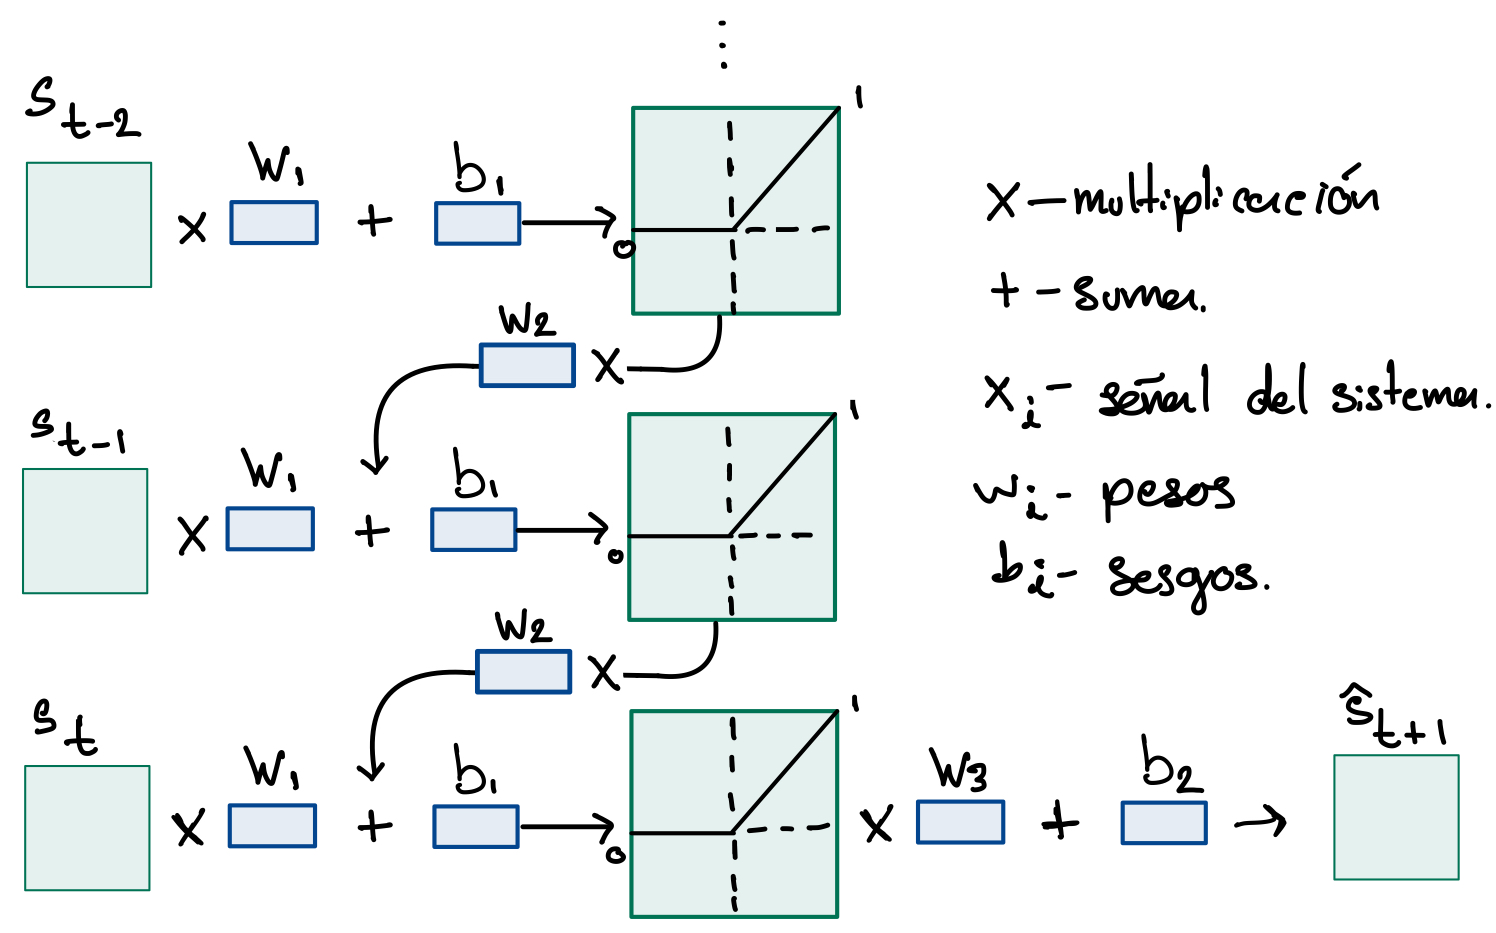
\includegraphics[width=0.8\linewidth]{arquitecturas/signal_rnn_diagrama.jpg}
    \caption{Estructura interna de una neurona recurrente, con funciones de activación ReLU.}
    \label{fig:rnn_estructura_neuronal}
\end{figure}

Las RNN's tienen como objetivo guardar información sobre todo el estado del sistema, paso a paso, hasta llegar al final de la ventana de $n$ observaciones definidas por el usuario, para generar la predicción $\hat{x}_{t+1}$ del estado futuro o todo un horizonte extendido, dados los $n$ pasos de contexto histórico. La estructura de esto se observa en en la figura \ref{fig:rnn_estructura_neuronal}.

\begin{align}
    s_{t+1} &= G \bigg(\big[ s_t \cdot w_1 + G(s'_{t-1})\cdot w_2 + b_1\big]\bigg)\cdot w_3 + b_2 \\
    s'_{t-1} &= s_{t-1}\cdot w_1+b_1+G( s'_{t-2}) \cdot w_2.
\end{align}

Para entender como surgió está idea, considere la ecuación diferencial ordinaria general, no lineal, de primer grado, no homogénea, que describe la evolución de la señal en un sistema a lo largo del tiempo.
\begin{equation}
    \frac{d\vec{s}(t)}{dt} = \vec{f}(t)+\vec{\phi}.
\end{equation}
$\vec{s}(t)$ es el valor del estado actual de la señal, dado el vector de dimensión $d$, $\vec{f}(t)$ es una función del tiempo, con $t\in \mathbb{R}^+$, y $\vec{\phi}$ es un vector constante de dimensión $d$. Esta ecuación se puede ver intuitivamente como la tasa de cambio del agua que hay en una cisterna, a la cual se le agrega agua conforme pasa el tiempo, y al mismo tiempo, está pierde agua durante el proceso; en un enfoque distinto, puede interpretarse como el cambio del precio de una acción.

Una forma de ver a $\vec{f}(t)$ es de la siguiente manera
\begin{equation}
    \vec{f}(t)=\vec{h}(\vec{s}(t) , \vec{x}(t)).
\end{equation}

donde $\vec{x}(t)$ es un vector de entrada de dimensión $d$ y $\vec{h}(\vec{s}(t) , \vec{x}(t))$ es una función vector-valuada que toma como entrada vectores-valuados.
Sustituyendo se tiene
\begin{equation}
    \frac{d\vec{s}(t)}{dt} = \vec{h}\big(\vec{s}(t) , \vec{x}(t)\big)+\vec{\phi}.
\end{equation}

Nuestro caso de interés, es cuando $f(t)$ es un modelo aditivo de la forma
\begin{equation}
\vec{f}(t) = \vec{a}(t) + \vec{b}(t) + \vec{c}(t)
\end{equation}
donde nuevamente sus términos son constituidos por funciones del tiempo de dimensión $d$. Como su nombre lo dice, añade sus términos, no lineales que determinan la tasa de cambio de la actividad neuronal, o sus potenciales $\vec{s}(t)$.

Considere ahora un modelo aditivo saturado, donde sus términos aditivos se definen de la siguiente manera.
\begin{align}
    \vec{a}(t) &= \sum_{k=0}^{K_s-1} \vec{a}_k \big(
    \vec{s}(t-\tau_s(k))  \big) \\
    \vec{b}(t) &= \sum_{k=0}^{K_r-1} \vec{b}_k \big(
    \vec{r}(t-\tau_s(k)) \big) \\
    \vec{r}\big(t-\tau_r(k)\big) &= G\big(\vec{s}(t-\tau_r(k)) \big) \\
    \vec{c}(t) &= \sum_{k=0}^{K_x-1} \vec{c}_k\big(
    \vec{x}(t-\tau_x(k))\big).
\end{align}
donde $\vec{r}(t)$ es el vector de la señal $\vec{s}(t)$ procesada por la función de activación $G(z)$, en la figura \ref{fig:rnn_estructura_neuronal} la función de activación es una ReLU, pero no está limitada a ella.\\

El sistema resultante es el siguiente
\begin{equation}
\begin{aligned}
    \frac{d\vec{s}(t)}{dt} &= \sum_{k=0}^{K_s-1} \vec{a}_k \big(
    \vec{s}(t-\tau_s(k))  \big) +  \sum_{k=0}^{K_r-1} \vec{b}_k \big(
    \vec{r}(t-\tau_s(k)) \big) \\
    &\quad + \sum_{k=0}^{K_x-1} \vec{c}_k\big(
    \vec{x}(t-\tau_x(k))\big) + \vec{\phi}.
\end{aligned}
\end{equation}
\begin{equation}
    \vec{r}\big(t-\tau_r(k)\big) = G\big(\vec{s}(t-\tau_r(k)) \big).
\end{equation}

El sistema anterior describe la tasa de cambio del estado $\vec{s}(t)$ como la combinación de diferentes efectos rezagados en el tiempo más un termino de sesgo.\\

Donde, el primer termino $\sum_{k=0}^{K_s-1} \vec{a}_k \big( \vec{s}(t-\tau_s(k))  \big)$ es el estado rezagado, donde versiones pasadas de este afectan el estado actual, lo que representa la memoria interna del sistema. Por otro lado, el segundo termino $\sum_{k=0}^{K_r-1} \vec{b}_k \big( \vec{r}(t-\tau_s(k)) \big)$ es similar al primer termino, solo que esta usa la salida transformada por la función de activación $(G)$, donde $\vec{r}(t)$ es una versión binarizada del estado $\vec{s}(t)$, lo que ayuda a reducir la distorsión. Puede interpretarse a como el perceptrón procesa la información antes de producir la salida. El penúltimo termino, $\sum_{k=0}^{K_x-1} \vec{c}_k\big( \vec{x}(t-\tau_x(k))\big)$ incorpora entradas externas rezagadas al sistema, lo que ayuda a modelar el estado $\vec{s}(t)$. Finalmente se tiene el ultimo termino $\vec{\phi}$ el cual representa el sesgo dentro del sistema. \\

En general, muchos procesos biológicos, físicos, económicos, entre otros;
usan frecuentemente valores pasados como predictores, donde la naturaleza de estos procesos
trae como consecuencia el uso de ecuaciones rezagadas para ser modelados de forma apropiada.
En el caso de las redes neuronales, los rezagos de las variables tanto de respuesta como
externas son una parte fundamental del sistema y uno de los factores principales que determinan las dinámicas del sistema. \\

Los términos rezagados que hemos visto representan la "memoria" del sistema, donde las
variables involucradas no dependen del momento actual, sino también de valores pasados,
medidos en diferentes momentos. Esto provoca que el sistema tenga en cuenta como ha cambiado
el sistema previamente, ademas de una señal derivada del estado que va acompañada de una forma
de la tangente hiperbólica la cual es una transformación no lineal, y además posea señales
externas que afectan al sistema, pero evaluadas en instantes previos.
Lo que enriquece la capacidad del modelo para capturar la relación causa-efecto y la influencia
del contexto temporal, dando como resultado una ecuación con una visión más completa de la historia
del sistema y cómo influye en el presente. \\

Ahora, suponiendo que $\vec{a}, \vec{b}$ y $\vec{c}$ son funciones lineales de $\vec{s}$, $\vec{r}$ y $\vec{x}$ respectivamente, entonces la ecuación se convierte en una ecuación diferencial no lineal de diferencias (DDE) con coeficientes lineales.
\begin{equation}
\begin{aligned}
    \frac{d\vec{s}(t)}{dt} &= \sum_{k=0}^{K_s-1} A_k \big(
    \vec{s}(t-\tau_s(k))  \big)\\
    &+  \sum_{k=0}^{K_r-1} B_k \big(
    \vec{r}(t-\tau_s(k)) \big)\\
    &+ \sum_{k=0}^{K_x-1} C_k\big(
    \vec{x}(t-\tau_x(k))\big) + \vec{\phi}.
\end{aligned}
\end{equation}

Al aplicar las siguientes condiciones  $K_s=1$, $\tau_s(0)=0$, $A_0 =A$, $K_r=1$, $\tau_r(0)=\tau_0$, $B_0=B$, $K_x=1$, $\tau_x(0)=0$, $C_0 = C$ a la ecuación anterior se tiene lo siguiente
\begin{equation}
    \frac{d\vec{s}(t)}{dt}=A\vec{s}(t)+B\vec{r}(t-\tau_0)+C\vec{x}(t)+\vec{\phi}.
\end{equation}
Estas ecuaciones son no-lineales de primer orden no-homogéneas. Una forma de evaluar estas ecuaciones es discretizar las en tiempo y calcular los valores de las señales de entrada y las señales de estado en cada momento sampleado hasta la duración total que se requiera, esto implica integración numérica. \cite{sherstinsky2020fundamentals}

Sea $\triangle T$ la duración total y $n$ el indice del tiempo en la aplicación de la regla discreta inversa de Euler aplicada a la ecuación anterior, por lo tanto

%% Modificar
\begingroup
 \smaller
\begin{gather}
    t= n\triangle T\\
    \frac{d\vec{s}(t)}{dt}\approx \frac{\vec{s}(n\triangle T + \triangle T) - \vec{s}(n\triangle T)}{\triangle T}\\
     A\vec{s}(t)+B\vec{r}(t-\tau_0)+C\vec{x}(t)+\vec{\phi} = A\vec{s}(n\triangle T)+B\vec{r}(n\triangle T-\tau_0)+C\vec{x}(n\triangle T)+\vec{\phi}\\
    \frac{\vec{s}(n\triangle T + \triangle T )-\vec{s}(n \triangle T)}{\triangle T} \approx A\vec{s}(n\triangle T + \triangle T)+B\vec{r}(n\triangle T+ \triangle T -\tau_0)+C\vec{x}(n\triangle T+ \triangle T)+\vec{\phi}.
\end{gather}
\endgroup

El valor de rezago $\tau_0$, sé iguala a un valor fijo, la razón de esto, es por que al avanzar, el contenido en la memoria se sobre escribe con un valor actualizado de la señal procesada, el cual se usará en el siguiente paso de tiempo, y así sucesivamente. Es por esto que se se establece $\tau_0=\triangle T$ y se reemplaza el signo de aproximación por el igual, de está manera se tiene...

\begingroup
\smaller
\begin{gather}
    \frac{\vec{s}(n\triangle T + \triangle T )-\vec{s}(n \triangle T)}{\triangle T} = A\vec{s}(n\triangle T + \triangle T)+B\vec{r}(n\triangle T)+C\vec{x}(n\triangle T+ \triangle T)+\vec{\phi}\\
    \frac{\vec{s}\big((n+1)\triangle T \big)-\vec{s}(n \triangle T)}{\triangle T} = A\vec{s}\big( (n+1)\triangle T\big)+B\vec{r}(n\triangle T)+C\vec{x}\big( (n+1)\triangle T\big)+\vec{\phi}\\
    \vec{s}\big((n+1)\triangle T \big)-\vec{s}(n\triangle T) = \triangle T \bigg(A\vec{s}\big( (n+1)\triangle T\big)+B\vec{r}(n\triangle T)+C\vec{x}\big( (n+1)\triangle T\big)+\vec{\phi}\bigg).
\end{gather}
\endgroup

Al aplicar discretización, todas las medidas de tiempo en la ecuaciones anterior se convierten en múltiplos integrales del paso de tiempo sampleando, $\triangle T$. Al eliminar $\triangle T$ de los argumentos, queda el eje de tiempo sin dimensión. Por lo tanto, todas las señales son transformadas en secuencias, cuyo dominio es el indice discreto $n$, y la ecuación 14 se convierte en una ecuación diferencial, no lineal, de primer orden y además, no homogénea. \cite{sherstinsky2020fundamentals}

\begingroup
\small
\begin{gather}
    \vec{s}[n+1] - \vec{s}[n]=\triangle T\bigg( A\vec{s}[n+1] + B\vec{r}[n] + C \vec{x}[n+1] + \vec{\phi}\bigg)\\
    \vec{s}[n+1]=\vec{s}[n]+\triangle T\bigg( A\vec{s}[n+1]+B \vec{r}[n]+C\vec{x}[n+1]+\vec{\phi} \bigg)\\
    \vec{s}[n+1]=\vec{s}[n]+\triangle T\cdot A\vec{s}[n+1]+\triangle T\cdot B \vec{r}[n]+ \triangle T\cdot C\vec{x}[n+1]+ \triangle T\cdot \vec{\phi}\\
    \vec{s}[n+1]-\triangle T\cdot A\vec{s}[n+1] = \vec{s}[n]+\triangle T\cdot B \vec{r}[n]+ \triangle T\cdot C\vec{x}[n+1]+ \triangle T\cdot \vec{\phi}\\
    (I-\triangle T \cdot A)\vec{s}[n+1]= \vec{s}[n]+\triangle T\cdot B \vec{r}[n]+ \triangle T\cdot C\vec{x}[n+1]+ \triangle T\cdot \vec{\phi}.
\end{gather}
\endgroup


Sea
\begin{equation}
    W_s=(I-\triangle T \cdot A)^-1,
\end{equation}
multiplicando la ecuación pasada por $W_s$ da como resultado
\begin{equation}
    \vec{s}[n+1]=W_s\vec{s}[n]+\triangle T\cdot W_s B \vec{r}[n]+ \triangle T\cdot W_s C\vec{x}[n+1]+ \triangle T\cdot W_s \vec{\phi}.
\end{equation}
restando uno al indice, la ecuación se transforma a
\begin{gather}
    \vec{s}[n]=W_s\vec{s}[n-1]+\triangle T\cdot W_s B \vec{r}[n-1]+ \triangle T\cdot W_s C\vec{x}[n]+ \triangle T\cdot W_s \vec{\phi}\\
    \vec{r}[n]= G\big(\vec{s}[n] \big).
\end{gather}
Ahora, se definen las siguientes matrices de pesos y vectores de sesgo,
\begin{gather}
    W_r=(\triangle T)B\\
    W_x=(\triangle T)C \\
    \vec{\theta}_s=(\triangle T)W_s\vec{\phi}.
\end{gather}
los cuales finalmente transforman el sistema en la forma canónica de la Red Neuronal Recurrente (RNN)

\begin{gather}
    \label{eq:eq_rnn_canonica}
    \vec{s}[n] = W_s \vec{s}[n-1] + W_r \vec{r}[n-1]+ W_x\vec{x}[n]+\vec{\theta}_s\\
    \vec{r}[n] = G(\vec{s}[n]).
\end{gather}

En la ecuación \ref{eq:eq_rnn_canonica}, note que la señal procesada por la función de activación vuelve alimentar a la célula en la siguiente observación, y esto ocurre varias veces, como se observa en la figura \ref{fig:rnn_estructura_neuronal}, lo que provoca que el gradiente se vuelva demasiado grande y este explote, o que de plano se de la desaparición forzada de este.

\cite{sherstinsky2020fundamentals} Escribe en su proposición 1, que una sola célula de la RNN, extendida por un numero finito de pasos, es computacionalmente capaz de encontrar a $\Theta$ tal que optimice $L$ sobre el conjunto de entrenamiento y que ademas pueda hacer inferencias sobre valores no vistos. \\

En general, surgen varios problemas con este sistema, el primero es que entre más observaciones existan en las secuencias de entrenamiento, la probabilidad que se obtengan buenos resultados aumenta, pero esto implica que aumentará la cantidad de cálculos computacionales que se tienen que realizar.\\

Por otra parte, si un sistema recurrente se extiende por una cierta cantidad de pasos pequeños, y es usado para predecir una secuencia de datos que exhibe tendencias de largo plazo, el sistema será entrenado bajo las hipótesis incorrectas, ya que este espera que los resultados de salida sean secuencias del mismo tamaño, donde en este caso es corto, por lo que la rnn no podrá capturar dependencias de largo plazo. \\

Uno de los problemas de las RNN's es que tras extenderlas a lo largo de varias observaciones, estás no logran pasar más allá de 5 a 10 pasos de acuerdo con \cite{sherstinsky2020fundamentals}. Esto se debe al hecho de que al entrenar esta red neuronal, los gradientes  tienden a crecer o disminuir con cada observación. Por lo que al transcurrir varias observaciones el gradiente explota o este se desvanece. El análisis detallado puede verse en \cite{sherstinsky2020fundamentals}


\subsection{Red Neuronal Recurrente con Memoria de Largo y Corto Plazo (LSTM)}

\begin{figure}[!h]
    \centering
    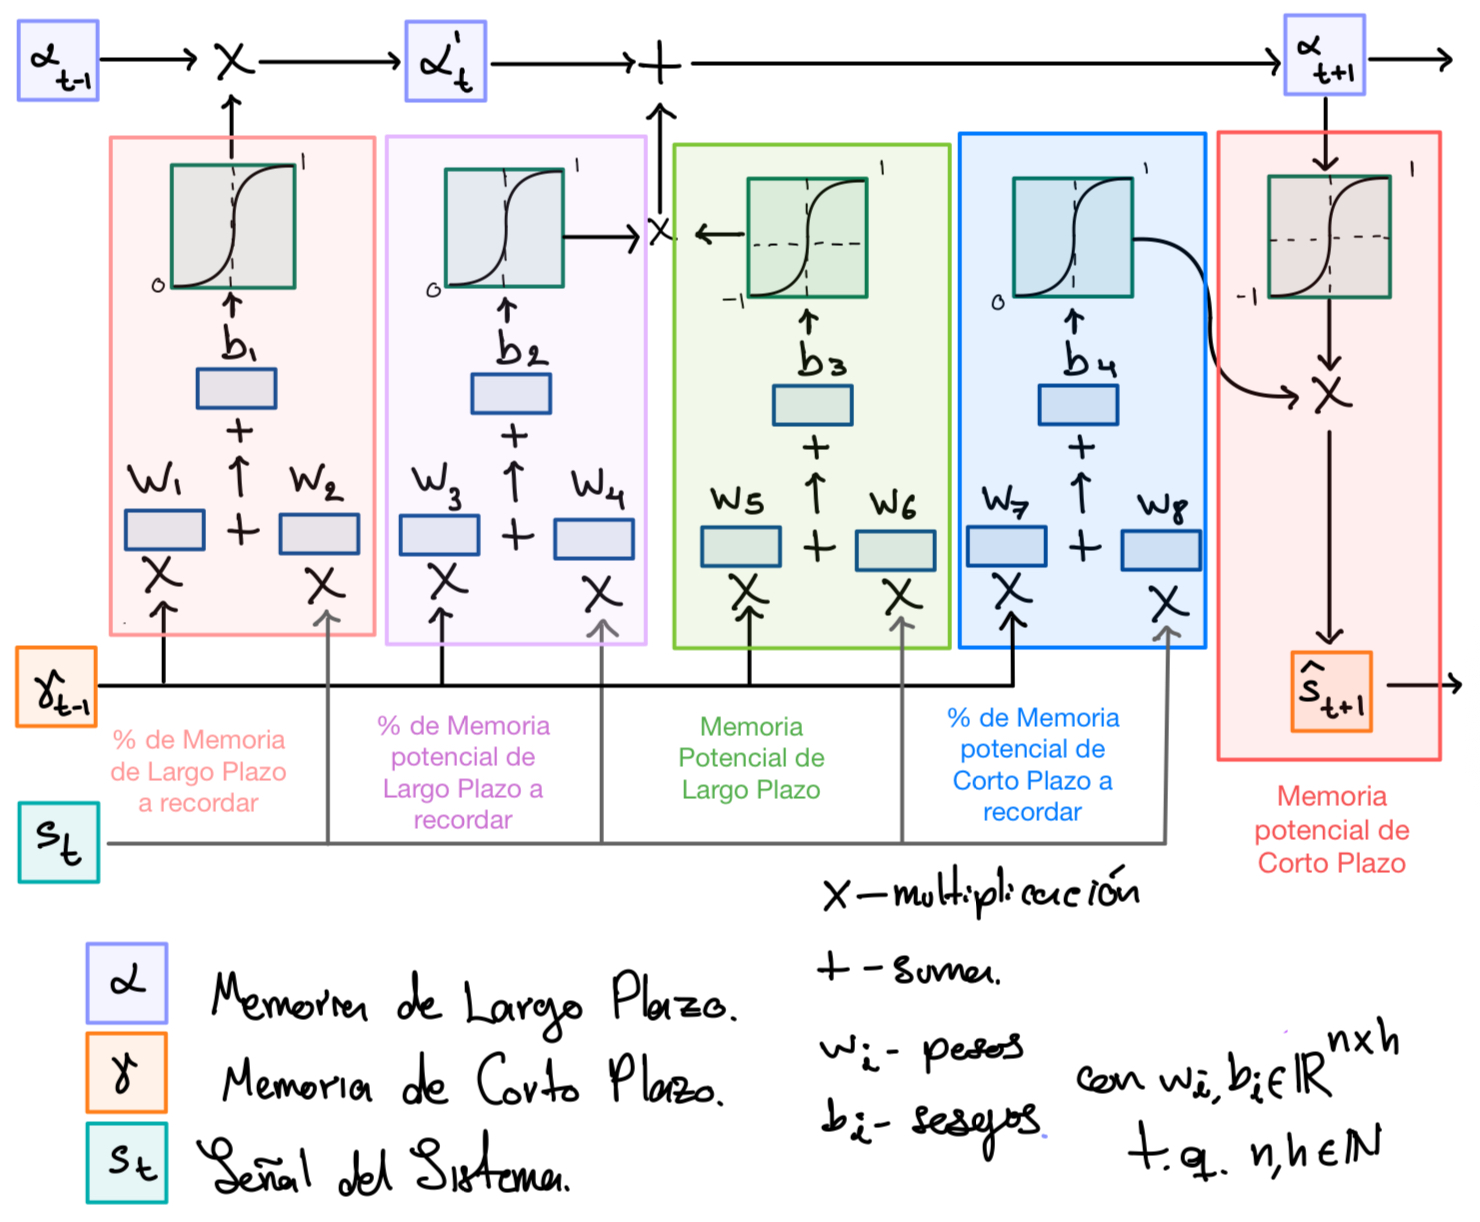
\includegraphics[width=0.8\linewidth]{arquitecturas/signal_lstm_diagrama.jpg}
    \caption{Estructura interna de una neurona recurrente}
    \label{fig:lstm_estructura_d_neurona}
\end{figure}

Las LSTMs surgen como la solución al problema de la desaparición y explosión de gradiente que ocurre cuando se entrena una RNN. Para ello se implemento un mecanismo que guarda dependencias temporales de corto como de largo plazo, de una forma no lineal dentro de la célula de la RNN, esto con la finalidad de que el gradiente de la función objetivo de la señal a modelar no se desvanezca o explote como ya mencionamos, véase la figura \ref{fig:lstm_estructura_d_neurona}.

El primer paso es separar la parte derecha de la ecuación 30.
\begin{align}
    \vec{s}[n] &= \vec{F}_s\big( \vec{s}[n-1] \big) + \vec{F}_u\big( \vec{r}[n-1], \vec{x}[n] \big)\\
    \vec{r}[n]&=G_d(\vec{s}[n])\\
    \vec{F}_s\big( \vec{s}[n-1] \big) &= W_s \vec{s}[n-1]\\
    \vec{F}_u\big( \vec{r}[n-1], \vec{x}[n] \big)&=W_r \vec{r}[n-1]+W_x\vec{x}[n]+\vec{\theta}_s.
\end{align}

donde nuevamente la función $G_d(\vec{z})$ es la tangente hiperbólica. Notese que en la ecuación 34, el estado de la señal se combina de forma igualitaria en cada observación, pero esto se puede ajustar al multiplicar ambas cantidades por "puertas especiales", $\vec{g}_{cs}[n]$ "control del estado" y $\vec{g}_{cu}[n]$ "control de actualización" respectivamente.
\begin{gather}
    \vec{s}[n]=\vec{g}_{cs}[n] \odot \vec{F}_s\big( \vec{s}[n-1] \big) + \vec{g}_{cu}[n] \odot \vec{F}_u\big( \vec{r}[n-1], \vec{x}[n] \big)\\
    \vec{0} \leq \vec{g}_{cs}[n], \vec{g}_{cu}[n] \leq \vec{1}.
\end{gather}

Los elementos de las señalas de las puertas son fracciones no negativas como se puede ver en la desigualdad de la ecuación 39. Por otro lado, la función $\vec{g}_{cs}[n]$ se encarga de controlar la cantidad de información del estado de la señal rezagado de la observación anterior, mientras que $\vec{g}_{cu}[n]$ regula la cantidad de información de la señal actualizada a ser inyectada en la observación actual. Finalmente, como $W_s$ es una matriz diagonal con entradas positivas fraccionarias $\frac{1}{|a_{ii}|}$ y dado que los elementos en $\vec{g}_{cs}[n]$ son también fracciones, se puede establecer a $W_s=I$ siempre y cuando las funciones de "puerta" sean paramétricas y sus parámetros sean aprendidos durante el entrenamiento, por lo que se puede simplificar la ecuación 36 a $F_s(\vec{s}[n-1])=\vec{s}[n-1]$\\

Véase ahora el termino de actualización $\vec{F}_u(\vec{r}[n-1], \vec{x}[n])$, el cuál es controlado por $\vec{g}_{cu}[n]$, nótese que en la ecuación 37, la función sigmoidal aplicada a la observación pasada del estado de la señal y la señal de la observación actual constituyen el candidato de actualización en cada observación con indice $n$, donde ambos términos contribuyen a ella en la misma proporción. El problema surge cuando $\vec{g}_{cu}[n] \sim 1$, ya que $\vec{s}[n-1]$ y $\vec{s}[n]$ se conectan a través de $W_r$ y la función sigmoidal $Gd$. está problemática limita al gradiente en la función objetivo respecto al estado de la señal, lo que trae como consecuencia al sistema la explosión o la desaparición forzada del gradiente, por lo que la función $\vec{r}[n]$ será controlada por otra puerta llamada "puerta de control" $\vec{g}_{cr}[n]$ de la siguiente manera
\begin{gather}
    \vec{v}[n] = \vec{g}_{cr}[n] \odot \vec{r}[n]\\
    \vec{0} \leq \vec{g}_{cr}[n] \leq \vec{1}.
\end{gather}
La puerta de control $\vec{g}_{cr}[n]$, determina el porcentaje de información de la función sigmoidal aplicado al estado de la observación pasada que será usado para la observación actual del estado $n$. Por lo que reemplazando $\vec{v}[n-1]$ por $\vec{r}[n-1]$ en la ecuación 37, está se transforma en
\begin{equation}
    \vec{F}_u\big( \vec{v}[n-1], \vec{x}[n] \big) = W_r\vec{v}[n-1] + W_x\vec{x}[n]+\vec{\theta}_s.
\end{equation}

Véase ahora que aun que la entrada externa $\vec{x}[n]$ no afecta a la estabilidad del sistema o contribuye al problema de la explosión del gradiente o su desaparición forzada, emparejar está entrada con otra puerta de control $\vec{g}_{cx}[n]$ única para si misma, ayuda al sistema a ser más flexible. Por lo que al incorporar esto en la ecuación anterior\dots
\begin{equation}
    \vec{F}_u\big( \vec{v}[n-1], \vec{x}[n] \big) = W_r\vec{v}[n-1] +  \vec{g}_{cx}[n]\odot W_x\vec{x}[n]+\vec{\theta}_s.
\end{equation}

Extendiendo por completo el sistema
\begin{equation}
    \vec{s}[n]=\vec{g}_{cs}[n] \odot \vec{s}[n-1] + \vec{g}_{cu}[n] \odot \big[ W_r\vec{v}[n-1] +  \vec{g}_{cx}[n]\odot W_x\vec{x}[n]+\vec{\theta}_s \big].
\end{equation}

Ahora, para hacer más robusto el sistema, resiliente y estable, se aplica una función no lineal de tipo tangente hiperbólica $G_d(z)$ a la señal agregada $\vec{F}_u\big( \vec{v}[n-1], \vec{x}[n] \big)$ lo que permite comprimir los valores y que estos se mantengan dentro del rango producido por la célula $\vec{v}[n]$ y la contribución de la señal de entrada $\vec{g}_{cx}[n] \odot \vec{x}_n$, el termino de actualización $\vec{u}[n]$ queda\dots
\begin{equation}
    \vec{u}[n]=G_d\big( F_u(\vec{v}[n-1], \vec{x}[n]) \big).
\end{equation}

Finalmente, sustituyendo el termino de actualización en la ecuación 44
\begin{equation}
    \vec{s}[n] = \vec{g}_{cs}[n]\odot \vec{s}[n-1] + \vec{g}_{cu}[n]\odot \vec{u}[n].
\end{equation}

La ecuación anterior es la culminación de todo el sistema de formulas que definen la red neuronal LSTM.\\

Los términos relacionados a las puertas de las señales $\vec{g}_{cs}[n], \vec{g}_{cr}[n]$ y $\vec{g}_{cu}[n]$ son en realidad funciones sigmoidal-es y tangentes hiperbólicas, cuyas expresiones matemáticas son las siguientes.

\begin{gather}
    \text{Sigmoide:} f(x)= \frac{e^x}{e^x+1}
\\
    \text{Hiperbólica Tangente:} f(x)=\frac{e^x-e^{-x}}{e^x+e^{-x}}
\end{gather}

% Añadir imagen de la función sigmoidal. y la tanh
Notese que estás funciones son diferenciables, monótonas crecientes, no lineales, continuas en todo su dominio $(-\infty , \infty)$ y cuyo rango comprende $(0,1)$ y $(-1,+1)$ respectivamente.

Véase ahora, que los términos que alimentaran las funciones de cada "puerta" son los siguientes
\begin{gather}
    \vec{z}_{cs}[n] = W_{x_{cs}}\vec{x}[n] + W_{s_{cs}}\vec{s}[n-1]+W_{v_{cs}} \vec{v}[n-1]+\vec{\theta}_{cs}\\
    \vec{z}_{cu}[n] = W_{x_{cu}}\vec{x}[n] + W_{s_{cu}}\vec{s}[n-1]+W_{v_{cs}} \vec{v}[n-1]+\vec{\theta}_{cu}\\
    \vec{z}_{cr}[n] = W_{x_{cr}}\vec{x}[n] + W_{s_{cr}}\vec{s}[n-1]+W_{v_{cr}} \vec{v}[n-1]+\vec{\theta}_{cr}
\end{gather}

Note que los valores que se emplean son todas las señales disponibles $\vec{s}[n-1], \vec{v}[n-1], \vec{x}[n]$, $\vec{s}[n], \vec{v}[n-1], \vec{x}[n]$ cercanas a la observación actual $n$.

Por lo tanto, las funciones de "puerta" quedan definidas como
\begin{gather}
    \vec{g}_{cs}[n]= G_c\big(\vec{z}_{cs}[n] \big)\\
    \vec{g}_{cu}[n]= G_c\big(\vec{z}_{cu}[n] \big)\\
    \vec{g}_{cr}[n]= G_c\big(\vec{z}_{cr}[n] \big)\\
\end{gather}

Esto hace que durante el entrenamiento y la inferencia, las puertas se vayan moldeando correspondientemente a las señales, al utilizar toda la información disponible en cada observación. Esto hace que las puertas detecten y mitiguen anomalías en las secuencias de entrada; haciendo el sistema de la lstm un modelo robusto que compensa las imperfecciones en los datos y capaz de generar secuencias de salida realmente buenas. \cite{apte2024advancing}

\subsection{DeepAr}

\begin{figure}[!h]
    \centering
    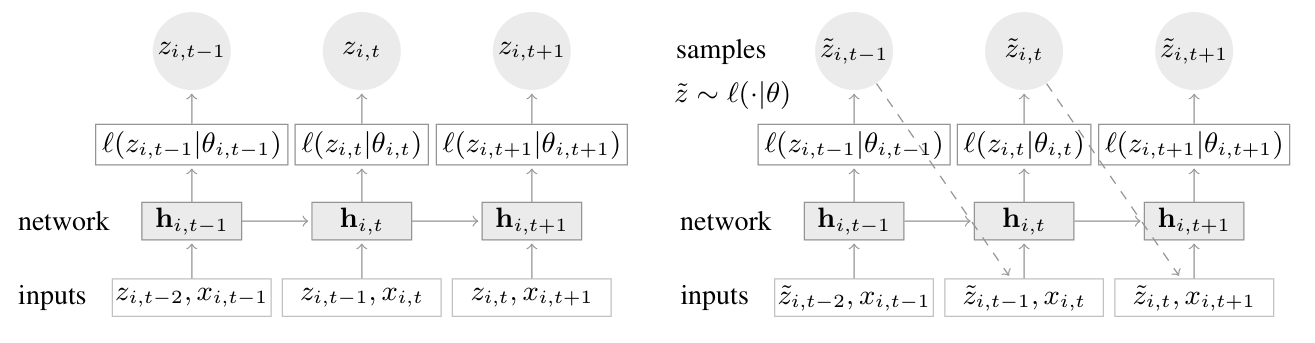
\includegraphics[width=0.9\textwidth]{arquitecturas/deeep_ar_imagen_modelo.png}
    \caption{Estructura de DeepAr, imagen de \cite{salinas2020deepar}}
    \label{fig:deepar_architecture}
\end{figure}

DeepAr es un modelo desarrollado por \textquotedblleft Amazon\textquotedblright \cite{salinas2020deepar}. DeepAr es un método basado en redes neuronales recurrentes autoregresivas que aprenden toda la historia de todas las series temporales en el conjunto de datos que se tenga, el cual utiliza LSTM's y una arquitectura similar al problema de predicción probabilístico. De acuerdo con los autores, DeepAr se luce al resolver el problema que se presenta al tratar de modelar múltiples series temporales, las cuales tienen diferentes características, principalmente, la continuidad y la escala de las mismas, así como también nuevas series temporales con pocos datos dada su incorporación reciente (Por ejemplo, la entrada de un producto al mercado, y que por consecuencia no se tienen información histórica de este.)

Tomando la notación de \cite{salinas2020deepar}, se denota el valor de una serie temporal con $i$ en el tiempo $t$ por $z_{i,t}$. El objetivo principal es modelar la distribución condicional de cada serie temporal que tendrá en el futuro $[z_{i,t_0}, z_{i,t_{0+1}}, \dots,z_{i,T}]:= \textbf{z}_{i,t_0:T}$, dado su pasado $[z_{i,1}, \dots, z_{i,t_0 - 2},z_{i,t_0-1}]:=\textbf{z}_{i, 1:t_0-1}$.

\begin{equation}
    P(\textbf{z}_{i,t_0:T} | \textbf{z}_{i,1:t_{0-1}}, \textbf{x}_{i,1:T})
\end{equation}
Donde $t_0$ denota la primer observación desconocida al momento de realizar la predicción, mientras que $\textbf{x}_{i,1:T}$ representa las variables conocidas en el futuro que explican la variable a ser predicha.

Como se menciona, el modelo se basa en la noción de probabilidad condicional, la cual indica que tan probable es un evento dada una condición.
\[
P(A|B) = \frac{P(A\cap B)}{P(B)}
\]
Esta distribución representa todas las posibles variantes futuras del sistema, ponderadas por su probabilidad de ocurrencia.

DeepAr se basa en una arquitectura auto-regresiva recurrente, en el sentido de que al predecir un valor $z_{i,t-1}$, toma ese mismo valor para alimentarse y obtener la siguiente predicción y al mismo tiempo toma el valor pasado de la salida de red $h_{i,t-1}$, tal como se vio con la RNN y la LSTM. Por otro lado asume que la distribución condicional de los valores futuros de las series temporales, consiste en el producto de distribuciones condicionadas, parametrizadas por la salida de la red $\textbf{h}_{i,t}$.
\begin{equation}
    Q_\Theta( \textbf{z}_{i,t_0:T} | \textbf{z}_{i,1:t_{0-1}}, \textbf{x}_{i,1:T})=\prod_{t=t_0}^T Q_\Theta(z_{i,t}|\textbf{z}_{i,t:t-1}, \textbf{x}_{i,1:T}) =\prod_{t=t_0}^T l\big( z_{i,t} |\theta(\textbf{h}_{i,t}, \Theta)\big)
\end{equation}
Donde
\begin{equation}
    \textbf{h}_{i,t}=h(\textbf{h}_{i,t-1}, z_{i,t-1},x_{i,t}, \Theta)
\end{equation}
hace referencia a la salida de una red neuronal lstm. En general el modelo admite $n$ capas LSTM con $m$ células por capa, con $n,m \in \mathbb{N}$. La salida de la red neuronal sirve para crear los parámetros de la distribución $l(z_{i,t}|\theta(\textbf{h}_{i,t}))$, a partir de la cual se infiere el valor futuro $z_{i,t}$.

Para ello se aplican dos transformaciones a la salida o estado oculto generado por la red $\textbf{h}_{i,t}$. Para el caso de una distribución normal, se predice la media y la desviación estándar de la siguiente manera
\begin{gather}
    l_G(z|\mu, \sigma) = (2\pi \sigma^2)^{-\frac{1}{2}}\exp\bigg(\frac{-(z-\mu)^2}{2\sigma^2}\bigg)\\
    \mu( \textbf{h}_{i,t})= \textbf{w}_\mu^T\textbf{h}_{i,t}+b_\mu\\
    \sigma( \textbf{h}_{i,t})=\log(1+\exp(\textbf{w}_\mu^T\textbf{h}_{i,t}+b_\mu))
\end{gather}
Mientras que para una distribución binomial negativa, está se parametriza por su media $\mu\in\mathbb{R}^+$ y el parámetro $\alpha\in\mathbb{R}^+$, permitiendo que de está manera la varianza dependa de la media $\text{Var}(z)=\mu+\alpha\mu^2$.
\begin{gather}
    l_{NB}(z|\mu,\sigma) = \frac{\Gamma(z+\frac{1}{\alpha})}{\Gamma(z+1) \Gamma(\frac{1}{\alpha})} \bigg( \frac{1}{1+\alpha \mu}\bigg)^{\frac{1}{\alpha}}\bigg( \frac{\alpha \mu}{1+\alpha\mu}\bigg)^z\\
    \mu(\textbf{h}_{i,t})=\log(1+\exp(\textbf{w}_\mu^T\textbf{h}_{i,t}+b_\mu))\\
    \sigma(\textbf{h}_{i,t})=\log(1+\exp(\textbf{w}_\sigma^T\textbf{h}_{i,t}+b_\sigma))\\
\end{gather}
En la practica se pueden usar diferentes distribuciones dependiendo el conjunto de datos y la distribución de estos, siempre y cuando sea fácil generar muestras de estás distribuciones, se pueda calcular el logaritmo de la función de verosimilitud con respecto a los parámetros, y los gradientes puedan ser evaluados con respecto a los parámetros del modelo para poder ser optimizados. En el caso de series temporales con valores positivos se suele usar la distribución binomial negativa.\\

Para entrenar el modelo, se parte de un conjunto de series temporales $\{\textbf{z}_{i, 1:T}\}_{i=1,\dots,N}$ junto con sus respectivas variables predictoras $\{\textbf{x}_{i,1:T}\}_{i=1,\dots,N}$. Se escoge un intervalo de tiempo en el que los valores $z_{i,t}$ dentro del horizonte de predicción sean conocidos, permitiendo calcular la función de pérdida basada en la verosimilitud.

Los parámetros del modelo, que incluyen tanto los pesos de la red neuronal recurrente $h(\cdot)$ como los parámetros de la función $\theta(\cdot)$ que mapea el estado oculto $h_{i,t}$ a los parámetros de la distribución de salida, pueden ser aprendidos mediante el algoritmo del descenso estocástico del gradiente. La función objetivo a maximizar es la log-verosimilitud total de las observaciones:

\begin{equation}
    \mathcal{L} = \sum_{i=1}^N \sum_{t=t_0}^T \log \ell(z_{i,t} \mid \theta(\textbf{h}_{i,t}))
\end{equation}

Dado que $h_{i,t}$ es una función determinista de las entradas, no se requiere inferencia sobre variables latentes, lo cual permite optimizar directamente la función de log-verosimilitud a través de gradientes computables con respecto a todos los parámetros del modelo.

En la practica, durante el entrenamiento, correspondiente al intervalo $t=1, \dots, t_0-1$, se va alimentando a DeepAr con las observaciones reales $z_{i,t}$ junto con las variables predictoras $x_{i,t}$ al modelo, el cual actualiza su estado oculto $\textbf{h}_{i,t}$ a través de una red lstm compartida. El último estado oculto $h_{i,t_0-1}$ toma la información relevante a toda la historia observada y sirve como un vector de contexto. A partir de ese estado inicial, comienza el proceso auto-regresivo, es decir, la generación de valores desconocidos, para el tiempo $t=t_0, \dots, T$, en donde DeepAr utiliza las predicciones pasadas $\hat{z}_{i,t}$ como entrada, junto con las variables predictoras $\textbf{x}_{i,t}$. Cabe recalcar que los parámetros de la LSTM son fijos y se comparten en el proceso general.

\subsection{Transformer}

El modelo Transformer, introducido por Vaswani et al. (2017), revolucionó el procesamiento de secuencias al eliminar por completo el uso de redes recurrentes. Su principal innovación es el mecanismo de atención, que permite capturar dependencias de largo alcance en las secuencias de entrada sin necesidad de procesarlas secuencial-mente. Esta arquitectura ha sido la base para múltiples avances en modelado secuencial, incluyendo su adaptación a series temporales como es el caso del modelo Informer.\\

El modelo fue diseñado originalmente con el objetivo de traducir oraciones a otro idioma. Su funcionamiento es totalmente distinto al acercamiento que se tiene con las redes neuronales recurrentes, o el caso probabilístico de DeepAr. Por lo que vale la pena incorporarlo a este experimento/investigación.

La arquitectura de transformer se divide en dos partes, el codificador y decodificador, para luego unirse; como se muestra en la siguiente figura.

%% Imagen Transformer
\begin{figure}[!h]
    \centering
    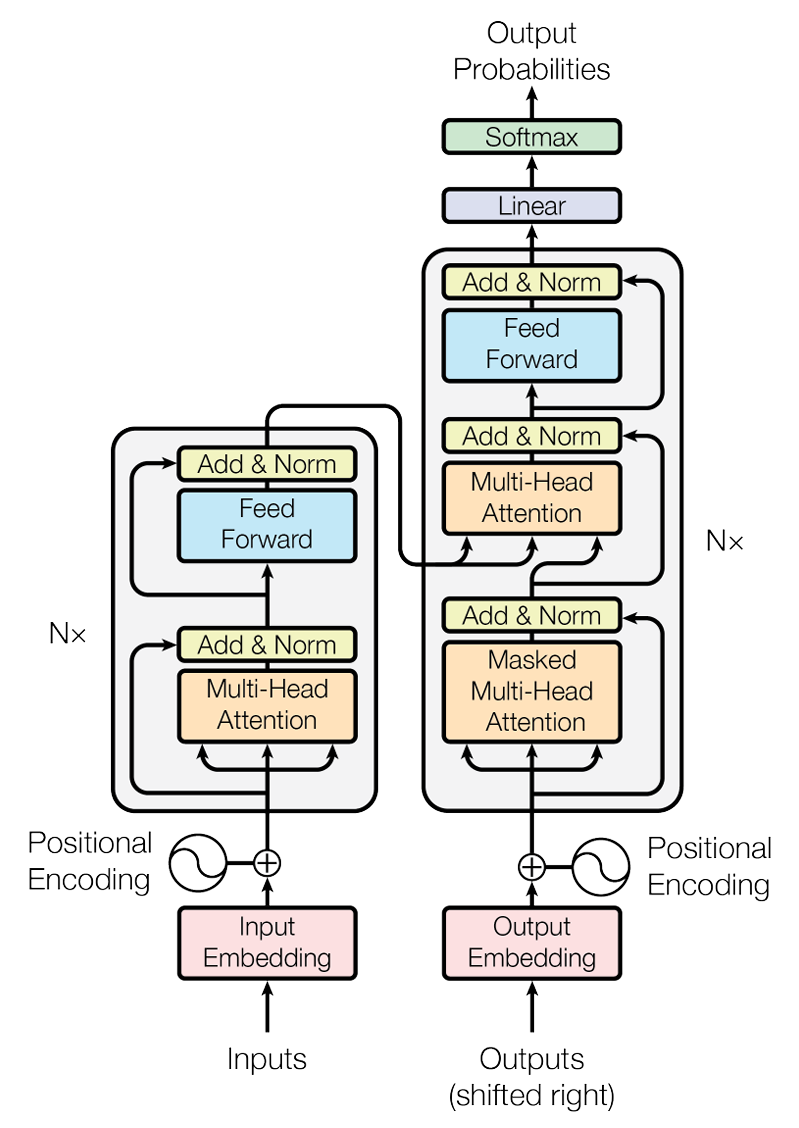
\includegraphics[width=0.5\textwidth]{arquitecturas/transformer_architecture.png}
    \caption{Arquitectura general del modelo Transformer, adaptado de Vaswani et al. (2017) \cite{vaswani2017attention}.}
    \label{fig:transformer_architecture}
\end{figure}

\subsubsection{Codificador}
La parte izquierda hace referencia al codificador, este se divide en 4 partes, la primer parte consiste en la transformación de palabras a números, ya que, una red neuronal solo procesa números. En el artículo \textit{Attention Is All You Need} establecen la dimensión del modelo como $d_{\text{model}} =512$, esto quiere decir que cada palabra se representará como un vector de dimensión 512 antes de poder se procesado por las capas de atención.


\subsubsection{Representación vectorial - Embeddings}
Como se menciono antes, dado que una red neuronal trabaja con números, cada palabra en el vocabulario definido en el entrenamiento, es representada de forma única por una matriz $W\in \mathbb{R}^{V \times d_{model}}$, donde $V$ corresponde a la cantidad única de palabras/``tokens" con las que el modelo fue entrenado. En \cite{} hay un total de $32,000$ tokens para el problema de traducción de Ingles - Alemán. Es importante mencionar, que en este aspecto, tanto el codificador como el decodificador poseen distintos vocabularios, por lo que cada vocabulario es codificado a su manera, con su respectiva matriz de pesos $W^{V_1}\in \mathbb{R}^{V_{1} \times d_{model}}$ y $W^{V_2} \mathbb{R}^{V_{2} \times d_{model}}$. Por otro lado, es importante mencionar que el vocabulario contiene tokens especiales.
\begin{center}
    \textless \text{PAD}\textgreater \,  $\rightarrow$ Relleno\\
    \textless START\textgreater  \,  $\rightarrow$ Inicio de la secuencia\\
    \textless EOS\textgreater \,  $\rightarrow$ Fin de la secuencia\\
    \textless UNK\textgreater \,  $\rightarrow$ Desconocido\\
\end{center}

Cuando se entrena el modelo, se construye un vocabulario, donde se ordena una lista de tokens (``palabras o sub-palabras") para que el modelo pueda procesarlos, como se muestra en la tabla \ref{tab:tokenizador}. De esta manera, cada palabra en una secuencia (una oración) es primero transformada en un número entero mediante un proceso de tokenización, basado en un vocabulario fijo de tamaño $V$. Este vocabulario asigna un índice único a cada palabra o subpalabra conocida por el modelo.

\begin{table}[t]
\begin{center}
\begin{tabular}{| c | c | c | c | }
\hline
\multicolumn{2}{ |c| }{Tokenización} \\ \hline
Índice & Token  \\ \hline
0 &  \textless PAD\textgreater\\
1 & \textless START\textgreater \\
2 & Carolina \\
3 & Sur \\
4 & Omelet \\
5 & come \\
\vdots & \vdots \\
V &  \textless EOS\textgreater\\ \hline
\end{tabular}
\caption{Ejemplo de la lista ordenada de todos los tokens (palabras) introducidos al modelo}
\label{tab:tokenizador}
\end{center}
\end{table}

 Véase este caso practico, dada la oración ``Carolina come un omelet", esta secuencia se divide, lo que da como resultado una secuencia de 4 palabras.
 \[
[\text{``Carolina''}, \text{``come''}, \text{``un''}, \text{``omele''}]
\]

Dentro de nuestro ejemplo,  ``Carolina'' corresponde al índice 2 en el tokenizador, por lo tanto, su representación inicial será un vector $\textbf{x}_{Carolina}=[0,0,1,\dots, 0] \in \mathbb{R}^V$. Luego, este será multiplicado por la matriz de embeddings $W\in \mathbb{R}^{V\times d_{model}}$ correspondiente al codificador. Finalmente, se obtiene el embedding final $\textbf{e}_{carolina}=\textbf{x}_{Carolina}\cdot W$. El proceso es análogo para el resto de palabras.
\begin{equation}
    \textbf{e}_i = \textbf{x}_i\cdot W
\end{equation}

\subsubsection{Codificación Posicional}
Ahora, es importante el orden en el que se van presentando las palabras, ya que no es lo mismo decir ``Carolina come un omelet'' a decir, ``Un omelet come Carolina'', ambas oraciones tienen las mismas palabras, pero ambas tienen un significado completamente distinto y además, se pierde el sentido en la última. La solución que se propone en \cite{vaswani2017attention} es utilizar una codificación posicional basada en funciones sinusoidales. Por lo que a cada posición \(pos\) en la secuencia de palabras se le asocia un vector \( \textbf{p}_{pos} \in \mathbb{R}^{d} \), al cual se le suma el embedding de la palabra correspondiente

\begin{equation}
\text{PE}_{(pos, 2i)} = \sin\left(\frac{pos}{10000^{\frac{2i}{d}}}\right), \quad
\text{PE}_{(pos, 2i+1)} = \cos\left(\frac{pos}{10000^{\frac{2i}{d}}}\right)
\end{equation}
donde \(pos\) es la posición de la palabra en la secuencia $(0,1,2, \dots)$, $i$ hace referencia a la dimensión en el vector del embedding y $d$ es la dimensión del vector.
De esta manera
\begin{equation}
    \tilde{\textbf{e}}_i = \textbf{e}_i + \textbf{p}_i
\end{equation}
donde $e_i\in\mathbb{R}^{d_{model}}$ es el embedding de la palabra, $\textbf{p}_i\in\mathbb{R}^{d_{model}}$ es el vector de codificación posicional dada la posición $i$. La ventaja de usar funciones de seno y coseno es que son cíclicas, además permiten capturar las diferencias relativas de acuerdo a su posición entre los elementos de la secuencia, y al mismo tiempo, se evita la necesidad de introducir más parámetros.

Si extendemos nuestra oración inicial a ``Carolina come un omelet con sur en un lindo lugar'' y aplicamos este principio a nuestra oración estableciendo la dimensión del modelo a 4, las funciones de seno y coseno se verían de la siguiente manera como se muestra en la Figura~\ref{fig:positional_encoding}.\\

\begin{figure}[!h]
    \centering
    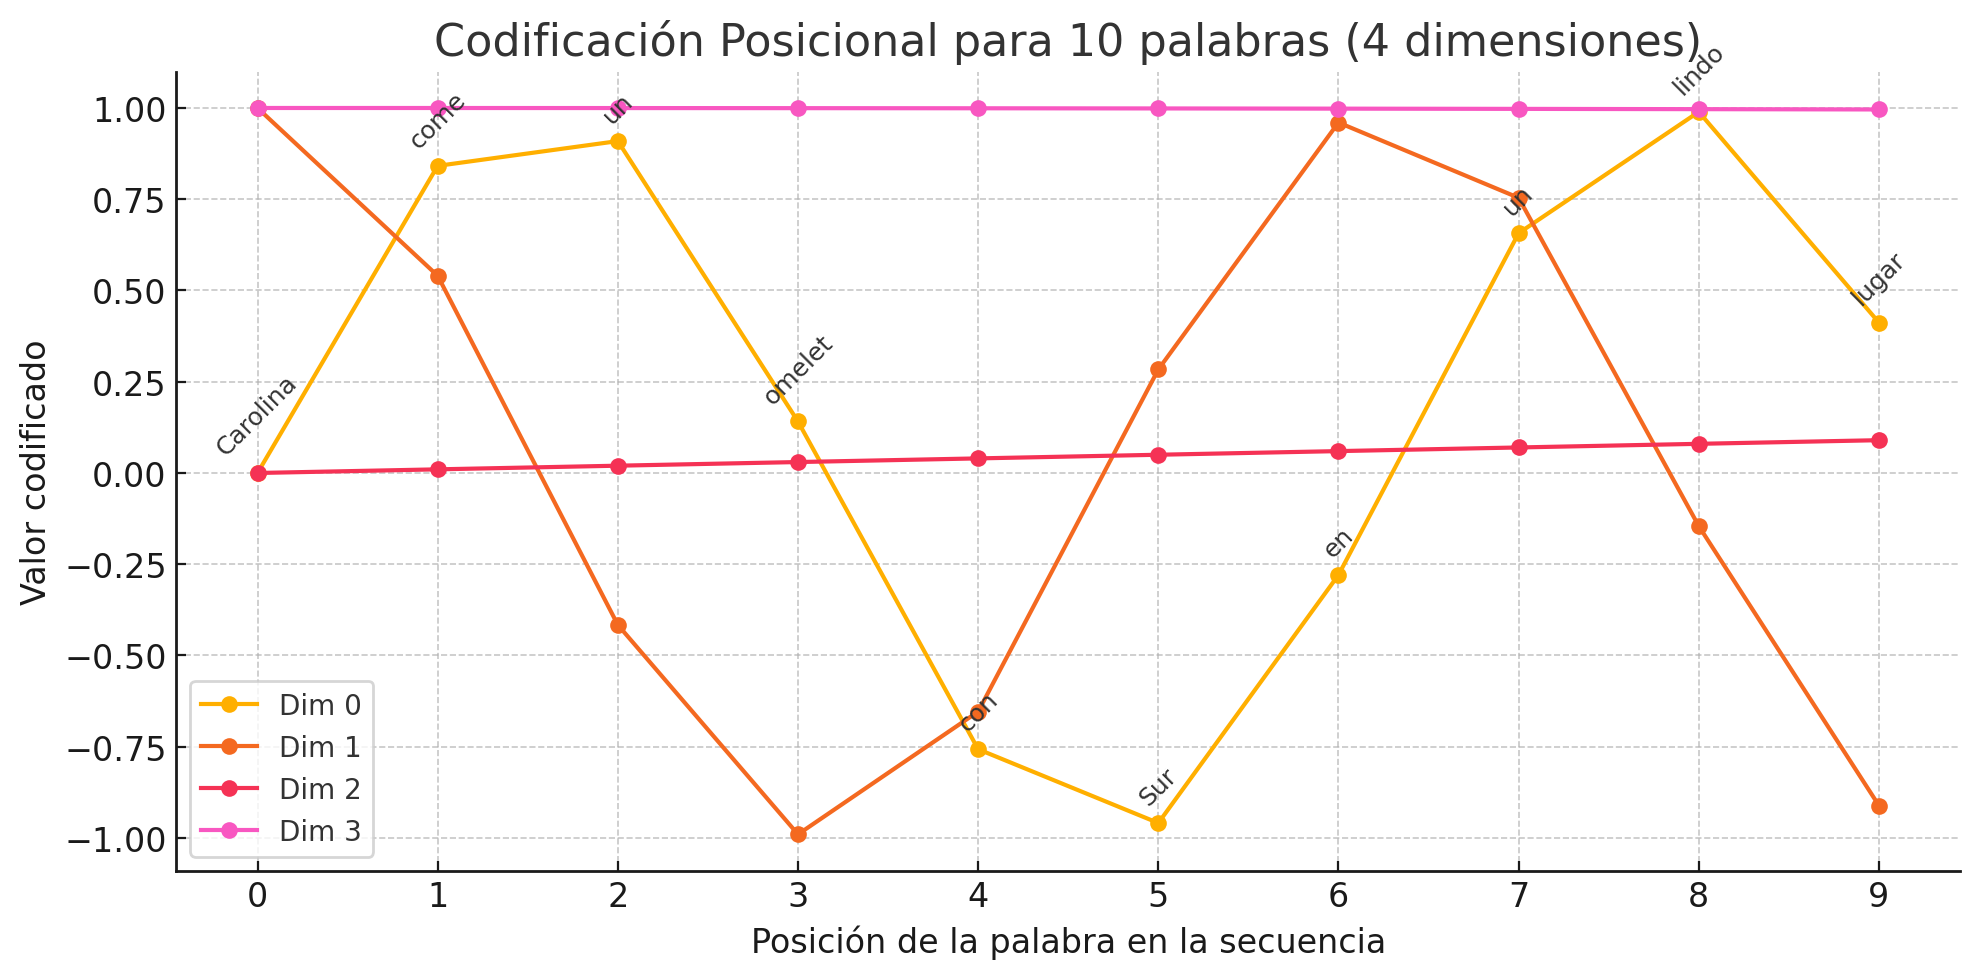
\includegraphics[width=0.8\textwidth]{sur_y_caro.png} % o .pdf según el archivo
    \caption{Codificación posicional para la oración \textit{``Carolina come un omelet con Sur en un lindo lugar''} con $d=4$. Cada dimensión representa una componente del vector posicional asociado a cada palabra, y varía según su posición en la secuencia.}
    \label{fig:positional_encoding}
\end{figure}

\subsubsection{Mecanismo de Atención}
Una vez que se tiene el posicionamiento codificado de cada palabra $\tilde{\textbf{e}}_i \in \mathbb{R}^{d_{\text{model}}}$, a cada una de ellas se le aplican tres transformaciones lineales con la finalidad de que cada una proporcione ``luz'' al modelo. Es por ello que en el mecanismo de atención que se define en \cite{vaswani2017attention} existen consultas $Q_i$ (``Queries''), llaves $K_i$ (``Keys'') y valores $V_i$ (``Values'') cada uno con una finalidad distinta.
\begin{gather}
    Q_i = \tilde{\textbf{e}}_i W^Q\\
    K_i = \tilde{\textbf{e}}_i W^K\\
     V_i = \tilde{\textbf{e}}_i W^V
\end{gather}
donde $W^Q, W^K, W^V\in \mathbb{R}^{d_{model}\times d_{model}}$, las consultas se encargan de resolver la pregunta ``¿Qué estoy buscando?'', mientras que las llaves ``¿Qué tengo para ofrecer?'' y el valor ``¿Qué puedo transmitir si soy relevante?''.

Para que el modelo pueda saber como se relacionan las palabras entre si, los autores \cite{vaswani2017attention} calculan la similitud (``score'') al hacer el producto punto entre la consulta de una palabra $Q_i$ contra todas las llaves $K_j$, incluida su propia llave.
\begin{equation}
    \text{score}_{i,j}=Q_i\cdot K_j
\end{equation}
De está manera se mide la afinidad o relevancia que hay entre la palabra en la posición $i$ y la palabra en $j$. Por otro lado, con la finalidad de que los valores no se vuelvan demasiado grandes y se sature la función exponencial normalizada (``softmax''), se escalan los valores al dividirlos entre la raíz cuadrada de $d_k$.
\begin{equation}
    \text{score escalado}_{i,j} = \frac{Q_i \cdot K_j}{\sqrt{d_k}}
\end{equation}
Luego, se aplica la función softmax a todas las puntuaciones $j$ para una posición $i$.
\begin{equation}
     \alpha_{i,j} = \text{softmax}\bigg( \frac{Q_i \cdot K_i}{\sqrt{d_k}} \bigg)
\end{equation}
De esta manera se generan pesos de atención, es decir, una distribución de probabilidad que le permite al modelo saber a qué otras palabras se les debe de ``atender''.
Finalmente, la salida de atención para la palabra $i$ se calcula como el promedio ponderado de los valores $V_j$.
\begin{equation}
    \text{Atención}_i = \sum_j \alpha_{i,j} V_j
\end{equation}
De esta forma, cada palabra tiene una nueva representación cuya dependencia se basa en el contexto de toda la secuencia. Este proceso se hace para todas las consultas de manera simultanea dentro de una matriz $Q$, así como las llaves $K$ y los valores $V$, por lo que de forma general se tiene
\begin{equation}
    \text{Atención}(Q, K, V) = \text{softmax}\big( \frac{QK^T}{\sqrt{d_k}} \big)V
\end{equation}
Esto conforma una sola función de atención con llaves, valores y consultas, donde $d_k=512=d_{model}$.

\subsubsection{Atención de Cabeza Múltiple - Multi-Head Attention }
Los autores \cite{vaswani2017attention} encontraron que en realidad es mucho mejor hacer $h$ proyecciones lineales con diferentes pesos en cada proyección con dimensiones $d_k = d_v = d_{\text{model}}/h=64$, con $h=8$ en el articulo de \cite{vaswani2017attention} donde $h$ representa la cantidad de cabezas de atención paralelas, cada una aprendiendo diferentes patrones en la secuencia. De esta manera es posible que secuencias de datos más largas y complejas puedan relacionarse mejor.
\begin{gather}
    \text{Multi-Atención}(Q, K, V) = \text{Concatenación}(\text{cabeza}_1, \dots, \text{cabeza}_h)W^{O}
\end{gather}
donde cada $\text{cabeza}_i = \text{Atención}(QW_i^Q, KW_i^K, VW_i^V)$ y las proyecciones $W_i^Q$, $W_i^K$, $W_i^V$ son matrices de pesos específicas para cada cabeza. Las salidas de cada cabeza son concatenadas y transformadas por una última matriz de pesos $W^O \in \mathbb{R}^{d_{\text{model}} \times d_{\text{model}}}$ que proyecta el resultado nuevamente al espacio original del modelo. Este mecanismo permite que el modelo atienda simultáneamente a distintas partes de la secuencia desde diferentes perspectivas, lo cual es clave para capturar relaciones semánticas complejas en estructuras de lenguaje o datos temporales.\\

Tras aplicar la Atención Multi-Cabeza, se tiene una salida por cada palabra, que se denotará por
\[
\text{MHA}(\tilde{\textbf{e}}_i)
\]
el cual es un vector de dimensión $d_{model}$.

\subsubsection{Conexiones Residuales}
La conexión residual consiste en sumar está salida con la entrada original, es decir, el vector codificado posicionalmente $\tilde{\textbf{e}}$ con $\text{MHA}(\tilde{\textbf{e}}_i)$. Esto se ve de la siguiente manera.
\begin{equation}
    \textbf{y}_i = \tilde{\textbf{e}}_i + \text{MHA}(\tilde{\textbf{e}}_i)
\end{equation}
En pocas palabras, el nuevo vector es el resultado de aplicar atención, sumando lo que ya se sabía. En general, una conexión residual ayuda a preservar la información original, evitando que se pierda lo que ya se sabe. Note que la conexión residual no bloquea el aprendizaje, pero si una capa no aprende nada útil aún durante el entrenamiento, al menos la entrada seguirá avanzando por el modelo.

\subsubsection{Capa de Normalización}
La capa de normalización (''Layer Normalization'' en ingles) ayuda acelerar el entrenamiento, mientras que estabiliza los valores evitando la explosión del gradiente o la desaparición forzada (como se ha visto anteriormente en las RNN's) y hace que las diferentes entradas del modelo permanezcan dentro de una misma escala. Esta se define de la siguiente forma
\begin{equation}
    \textbf{z}_i=\text{LayerNorm}(\textbf{y}_i ) = \gamma \cdot \frac{\textbf{y}_i - \mu}{\sqrt{\sigma^2+\epsilon}}+\beta
\end{equation}
Donde, $\mu=\frac{1}{d}\sum_{j=1}^d y_{ij}$ es la media del vector $\textbf{y}_i$, $\sigma^2=\frac{1}{d}\sum_{j=1}^d(y_{ij}-\mu)^2$ es la varianza, $\gamma, \beta \in \mathbb{R}^{d_{model}}$ son parámetros aprendidos, y $\epsilon$ es un valor pequeño para prevenir la división por cero.

\subsubsection{Capa Feed-Forward por posición}
Está capa se compone por dos transformaciones lineales con una activación ReLU en medio. Estas transformaciones se aplican de manera separada e idéntica a cada posición en la secuencia. De acuerdo con \cite{vaswani2017attention}, esta operación se describe de la siguiente manera:
\begin{equation}
    \text{FFN}(x)=\text{ReLU}(xW_1+b_1)W_2+b_2
\end{equation}
Donde $x\in \mathbb{R}^{d_{model}}$ es el vector de entrada, que hace referencia a una palabra que ya ha sido procesada por la capa de atención múltiple, más la suma de su posición codificada y además de estar normalizada, mientras que $W_1\in \mathbb{R}^{512\times 2048}$ y $W_2 \in \mathbb{R}^{2048\times 512}$. Note que la dimensión intermedia $d_{ff}=2048$ contribuye a que exista una expansión temporal de características, seguida de una compresión para regresar a la dimensión original.

En nuestro ejemplo siguiendo el proceso de una palabra, esto luce así
\begin{equation}
    \textbf{f}_i =\text{FFN}(\textbf{z}_i) = \text{ReLU}(\textbf{z}_iW_1+b_1)W_2+b_2
\end{equation}

\subsubsection{Conexión Residual y Capa de Normalización}
Una vez aplicada la capa Feed-Forward por posición, se realiza nuevamente una conexión residual, y se aplica normalización.
\begin{gather}
    \textbf{u}_i = \textbf{z}_i + \textbf{f}_i = \text{LayerNorm}(\textbf{y}_i) + \text{ReLU}(\textbf{z}_iW_1+b_1)W_2+b_2\\
    \textbf{e}_{i_{enc}} = \text{LayerNorm}(\textbf{u}_i)
\end{gather}
Esto culmina el proceso del codificador aplicado a una sola palabra. En general, todos los cálculos se hacen con matrices, lo que facilita el proceso de entrenamiento ya que todo se hace en paralelo.

\subsubsection{Sistema Completo - Codificador}
Dada una secuencia de $n$ palabras, cada una codificada como un vector ``one-hot'' de longitud $V$ se tiene la matriz $X\in \mathbb{R}^{n\times V}$.
\begin{gather}
    E=XW \quad \text{donde} \,\,W \in \mathbb{R}^{V\times d_{model}}\\
    \tilde{E}=E+P \quad \text{(P es la matriz de codificación posicional)}\\
    \text{MHA}(\tilde{E})=\text{Concat}\big(\text{Atención}_i(Q=\tilde{E}W_i^Q,K=\tilde{E}W_i^K,V=\tilde{E}W_i^V)\big)W^O\\
    Y=\tilde{E}+\text{MHA}(\tilde{E})\\
    Z=\text{LayerNorm}(Y)\\
    F=\text{FFN(Z)}\\
    U = Z+F\\
    E_{enc} = \text{LayerNorm}(U)
\end{gather}

\subsubsection{Decodificador}
El decodificador es la parte del modelo encargada de generar la secuencia de salida de manera autoregresiva, es decir, un elemento a la vez. Su estructura es semejante a la del codificador, pero con dos cambios importantes.
\begin{enumerate}
    \item Enmascarada la atención, para evitar que el modelo acceda a tokens futuros durante el entrenamiento.

    \item Se introduce el bloque de atención cruzada, el cual permite que el decodificador; consulte la salida del codificador.
\end{enumerate}

\subsubsection{Embeddings de entrada al decodificador}
De forma análoga al codificador, el decodificador también transforma los tokens de salida generados hasta el momento en vectores numéricos mediante una matriz de embeddings. Para cada posición \( i \), el token correspondiente se transforma en un vector \( \textbf{e}_i \in \mathbb{R}^{d_{\text{model}}} \), al cual se le suma una codificación posicional \( \textbf{p}_i \) para preservar el orden:
\begin{equation}
\tilde{\textbf{e}}_i = \textbf{e}_i + \textbf{p}_i
\end{equation}
Este vector \( \tilde{\textbf{e}}_i \) representa la entrada final al decodificador para la posición \( i \), y se utiliza como punto de partida para los mecanismos de atención autoregresiva que siguen a continuación.

\subsubsection{Atención enmascarada en el decodificador}
Cuando se aplica atención en el codificador, cada posición puede atender a cualquier otra en la secuencia de entrada, incluso hacia adelante. Pero en el decodificador esto no se puede; de lo contrario, el modelo estaría haciendo trampa, ya que se estarían utilizando palabras futuras para predecir la actual. De manera particular, como la entrada al decodificador es el vector $\tilde{\textbf{e}}_i$, este se transforma en tres representaciones distintas.
\begin{equation}
Q_i = \tilde{\textbf{e}}_i W^Q, \quad K_j = \tilde{\textbf{e}}_j W^K, \quad V_j = \tilde{\textbf{e}}_j W^V
\end{equation}
donde \( j \le i \), ya que solo se puede atender a palabras anteriores o a sí misma.
Luego se calcula la atención enmascarada para la posición \( i \) de la siguiente manera.
\begin{equation}
\text{Atención}_i = \sum_{j=1}^{i} \alpha_{i,j} V_j, \quad \text{donde } \alpha_{i,j} = \text{softmax}_j\left( \frac{Q_i \cdot K_j}{\sqrt{d_k}} \right)
\end{equation}
Como ya se ha visto, en general se usan matrices para hacer el entrenamiento más rápido y de forma paralela, por lo que la operación matricial es análoga a la que se emplea en el codificador como muestra:
\[
Q = \tilde{E}_{\text{dec}} W^Q, \quad K = \tilde{E}_{\text{dec}} W^K, \quad V = \tilde{E}_{\text{dec}} W^V
\]
donde \( \tilde{E}_{\text{dec}} \in \mathbb{R}^{n_{\text{dec}} \times d_{\text{model}}} \) es la secuencia completa de embeddings codificados posicionalmente. Por otro lado, la atención enmascarada se calcula de forma similar a la atención definida en el codificador, solo que en este caso se suma una matriz cuadrada $M$.
\begin{equation}
\text{Atención Enmascarada}(Q, K, V) = \text{softmax}\left( \frac{Q K^\top}{\sqrt{d_k}} + M \right)V
\end{equation}

donde \( M \in \mathbb{R}^{n \times n} \) es una máscara triangular inferior:

\[
M_{i,j} =
\begin{cases}
0 & \text{si } j \le i \\
- \infty & \text{si } j > i
\end{cases}
\]
\[
M=
\begin{pmatrix}
0 & -\infty & -\infty& \dots & -\infty\\
0 & 0 & -\infty& \dots & -\infty\\
0& 0 & 0 & \dots &-\infty\\
\vdots &\vdots &\vdots & \ddots & \vdots\\
0 & 0 & 0 & \dots& 0
\end{pmatrix}
\]
De esta manera, al aplicar la función Softmax, los elementos enmascarados con $-\infty$ hacen que su probabilidad se vaya a 0, lo que garantiza que el modelo solo pueda usar información de tokens ya generados hasta el momento. Al igual que en el codificador, esta atención se implementa en múltiples cabezas paralelas y luego se combinan mediante una proyección lineal.

Se denotará a la salida individual por $\text{Masked-MHA}(\tilde{\textbf{e}}_i)$, mientras que a la salida matricial por $\text{Masked-MHA}(\tilde{\textbf{E}}_{dec})$

\subsubsection{Conexión Residual y Normalización}
Luego de aplicar la atención enmascarada, se vuelve a incorporar una conexión residual, para luego normalizar la suma del embedding del decodificador $\tilde{\textbf{e}}_i$ y la salida de la atención enmascarada $\text{Masked-MHA}(\tilde{\textbf{e}}_i)$.
\begin{gather}
    \textbf{y}_i= \tilde{\textbf{e}}_i + \text{Masked-MHA}(\tilde{\textbf{e}}_i)\\
    \textbf{z}_i = \text{LayerNorm}(\textbf{y}_i)
\end{gather}

\subsubsection{Atención cruzada (Encoder–Decoder Attention)}
En este punto, el decodificador contiene información generada de manera autoregresiva por medio de $\textbf{z}_i$, pero aún no incorpora ningún conocimiento acerca de la secuencia de entrada procesada por el codificador. Para integrar está información, se introduce el mecanismo de atención cruzada. En esta etapa, la secuencia generada hasta el momento actúa como una consulta, mientras que las salidas del codificador funcionan como llaves y valores. El objetivo es permitir que el decodificador seleccione dinámicamente qué partes de la entrada codificada son más relevantes para generar cada token de salida.

Por lo tanto, la representación $\textbf{z}_i$ se transforma en una consulta al ser mutiplicada por la matriz $W^Q$ como se muestra:
\begin{equation}
Q_i = \textbf{z}_i W^Q
\end{equation}
Mientras que las representaciones de la entrada, procesadas previamente en el codificador y almacenadas en la matriz $E_{\text{enc}}$, son proyectan a llaves y valores:
\begin{equation}
K_j = E_{\text{enc},j} W^K, \quad V_j = E_{\text{enc},j} W^V
\end{equation}
Por lo tanto, la atención cruzada para la posición $i$ se calcula como:
\begin{equation}
\text{Atención}_i = \sum_{j=1}^{n_{\text{enc}}} \alpha_{i,j} V_j, \quad \text{donde } \alpha_{i,j} = \text{softmax}_j\left( \frac{Q_i \cdot K_j}{\sqrt{d_k}} \right)
\end{equation}

Generalizando para toda la secuencia, se tienen las matrices:
\begin{gather}
Q = Z_{\text{dec}} W^Q, \quad K = E_{\text{enc}} W^K, \quad V = E_{\text{enc}} W^V\\
\text{Atención Cruzada}(Q, K, V) = \text{softmax}\left( \frac{Q K^\top}{\sqrt{d_k}} \right)V
\end{gather}
Esta salida se suma de forma residual a la entrada del decodificador y se normaliza:
\begin{equation}
\textbf{o}_{\text{dec}} = \text{LayerNorm}(Z_{\text{dec}} + \text{Atención Cruzada}(Q, K, V))
\end{equation}

Esto permite que el modelo combine la información autoregresiva generada en el decodificador con la información codificada de la secuencia de entrada, guiando de forma efectiva el proceso de generación.

\subsubsection{Capa Feed-Forward por posición}
Véase que $\textbf{o}_{\text{dec}}$ contiene tanto la información autoregresiva generada hasta ese momento, como la información relevante de la secuencia de entrada. Por lo que el siguiente paso consiste en transformar esta representación mediante una red neuronal completamente conectada, justo como ocurrió en el codificador.
\begin{equation}
\text{FFN}(\textbf{o}_i) = \text{ReLU}(\textbf{o}_i W_1 + b_1) W_2 + b_2
\end{equation}
Finalmente, como es costumbre tras aplicar atención, se aplica una conexión residual y una normalización por capa.
\begin{align}
\textbf{u}_i &= \textbf{o}_i + \text{FFN}(\textbf{o}_i) \\
\textbf{h}_i &= \text{LayerNorm}(\textbf{u}_i)
\end{align}
De forma matricial
\begin{equation}
\textbf{H}_{\text{dec}} = \text{LayerNorm}(\textbf{O}_{\text{dec}} + \text{FFN}(\textbf{O}_{\text{dec}}))
\end{equation}
donde \( \textbf{O}_{\text{dec}} \in \mathbb{R}^{n_{\text{dec}} \times d_{\text{model}}} \) es la matriz que contiene las representaciones finales de cada posición tras aplicar atención cruzada.

\subsubsection{Predicción final y generación autoregresiva}
La salida del decodificador luego de atravesar todo el sistema es una matriz \( \textbf{H}_{\text{dec}} \in \mathbb{R}^{n_{\text{dec}} \times d_{\text{model}}} \), donde cada fila representa la codificación final de una posición en la secuencia generada. El objetivo principal ahora es convertir estas representaciones en predicciones de tokens del vocabulario $V$ definido desde el inicio.

Para ello, se aplica una proyección lineal que transforma cada vector de dimensión \( d_{\text{model}} \) en un vector de puntuaciones ("logits") de dimensión \( V \), el tamaño del vocabulario:
\begin{equation}
\textbf{logits}_t = \textbf{h}_t W^{\text{out}} + b^{\text{out}}, \quad \text{con } W^{\text{out}} \in \mathbb{R}^{d_{\text{model}} \times V}
\end{equation}
Luego, se aplica la función softmax para convertir estas puntuaciones en una distribución de probabilidad sobre todos los tokens posibles:
\begin{equation}
\textbf{p}_t = \text{softmax}(\textbf{logits}_t) \in \mathbb{R}^{V}
\end{equation}

El token con mayor probabilidad es seleccionado como predicción para la posición \( t \). Este proceso se repite paso a paso de manera autoregresiva: en cada iteración, el token generado se concatena a la secuencia de entrada al decodificador, permitiendo que se prediga el siguiente token. Este ciclo continúa hasta que se alcanza un token especial de fin de secuencia \( <\texttt{EOS}> \) o se supera una longitud máxima.

Durante la fase de entrenamiento, este proceso se acelera mediante el uso de la secuencia de salida completa en paralelo, enmascarando las posiciones futuras con una máscara triangular inferior. En cambio, durante la inferencia, el modelo genera la secuencia \textbf{token} por \textbf{token}.

\subsection{D$^3$VAE}

\begin{figure}[!h]
    \centering
    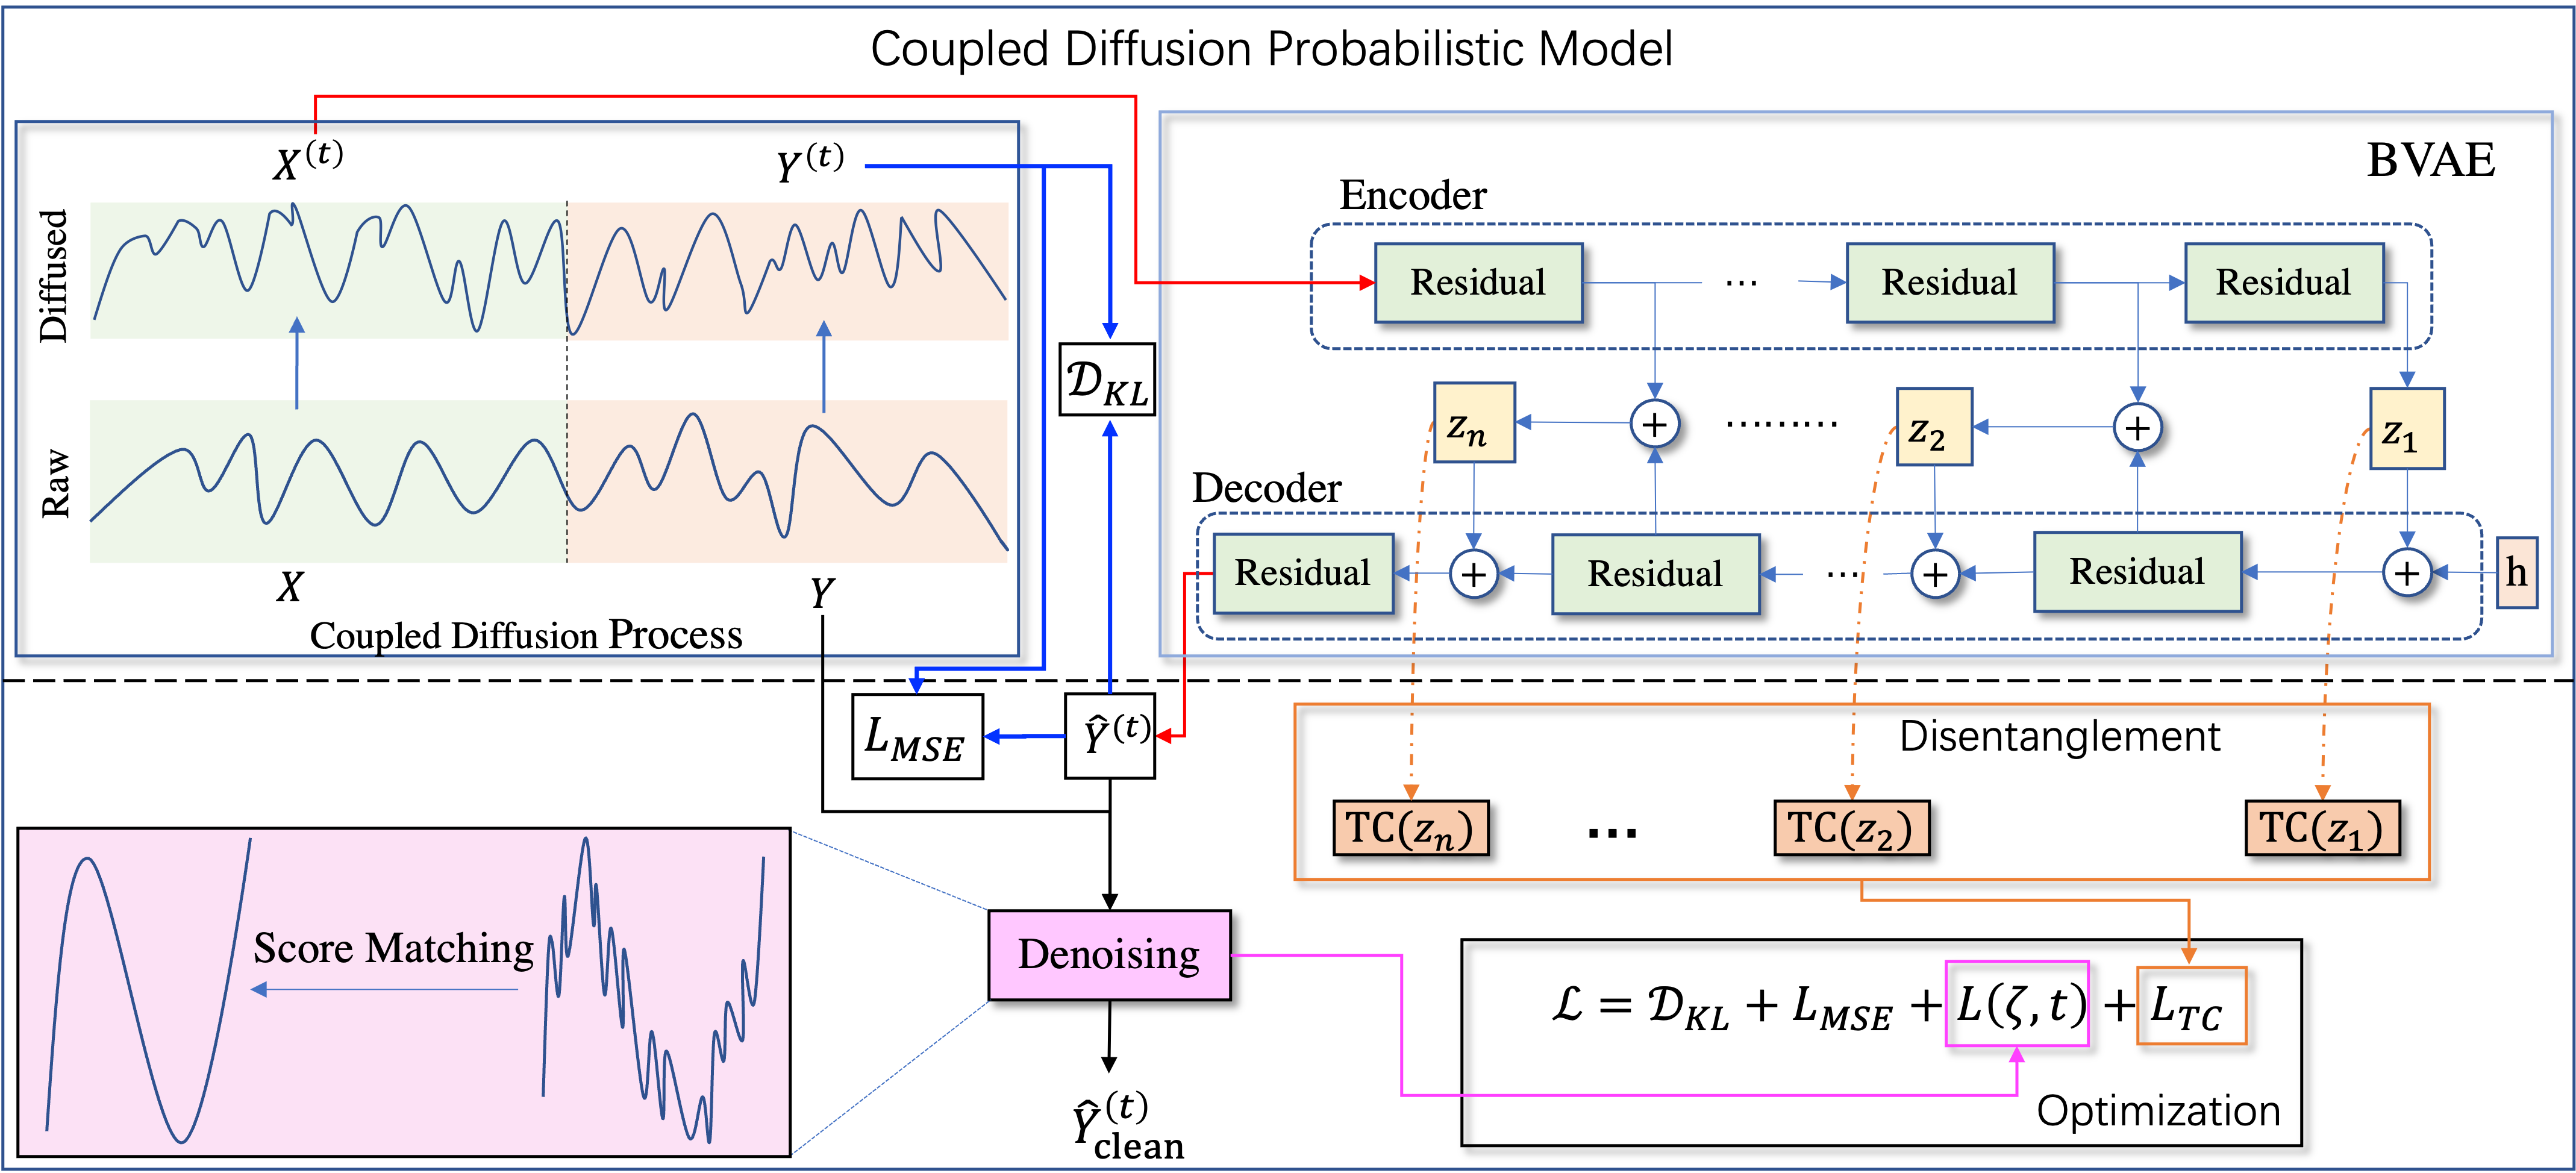
\includegraphics[width=0.8\textwidth]{arquitecturas/framework.png}
    \caption{Estructura de DVAE, imagen de \cite{li2022generative}}
    \label{fig:dvae_architecture}
\end{figure}

El modelo D³VAE busca modelar la distribución de la serie temporal observada $x$ como una función de variables latentes $z$, las cuales se asumen provenientes de una distribución gaussiana multivariada. A diferencia de los modelos clásicos, D³VAE introduce un proceso de difusión acoplado con técnicas de denoising score matching y una estrategia de disentanglement en el espacio latente. Esto permite una generación más robusta y estructurada de series temporales, manteniendo consistencia temporal y separando distintos patrones dinámicos presentes en los datos (tendencia, estacionalidad, etc.).

\subsubsection{Formulación del Problema}
Considérese una serie temporal multivariada $X=\{ x_1, \dots, x_n\}$, donde cada $x_i\in \mathbb{R}^d$ representa un conjunto de $d$ variables predictoras, incluyendo la variable de respuesta, y sea $Y=\{y_{n+1}, \dots, y_{n+m}\}$ la variable de respuesta que se desea pronosticar.
Se asume la existencia de una variable latente $Z\sim p(Z|X)$ desde la cual se puede generar la distribución de la serie objetivo mediante una función paramétrica $f(\cdot)$. De esta forma, la distribución de $Y$ queda definida como\dots
\begin{equation}
    p(\mathbf{Y}) = \int p(\mathbf{Z}|\mathbf{X}) \cdot p(\mathbf{Y} | f(\mathbf{Z})) , d\mathbf{Z}
\end{equation}
Por lo tanto, el objetivo principal del modelo es aprender una representación latente $Z$ que capture las señales importantes de $X$ que permitan reconstruir de forma precisa la serie futura $Y$.

\subsubsection{Preposición 1: Descomposición de señal y ruido}
Sea $X$ una serie temporal multivariada de entrada, y sea $X_r$ su componente ideal, es decir, libre de ruido. Suponga que toda serie temporal puede descomponerse como...
\begin{equation}
    X = X_r + \epsilon_X
\end{equation}
Donde $\epsilon_X$ representa el ruido inherente a las observaciones, y se asume que $X_r \bot \epsilon_X$, es decir, son estadísticamente independientes.

Bajo esta suposición, la distribución de la variable $Z$, condicionada a $X$, puede expresar como\dots
\begin{equation}
    p(Z|X)=p(Z|X_r, \epsilon_X)
\end{equation}
Del mismo modo, la serie objetivo $Y$ puede descomponerse como
\begin{equation}
    Y = Y_r + \epsilon_Y
\end{equation}
donde $Y_r$ es la parte ideal de la variable de respuesta, y $\epsilon_Y$ representa el ruido en la salida. (tal como la aleatoriedad, errores de medición, o factores modelados).

El modelo se entrena para capturar completamente $Y_r$, es decir, se asume que puede modelarse sin error.

\begin{equation}
    \hat{Y}_r\approx Y_r
\end{equation}
Entonces, el error total entre la predicción y la variable de respuesta es
\begin{equation}
    ||\hat{\textbf{Y}}  -\textbf{Y}||=||\hat{\textbf{Y}}_r + \epsilon_{\hat{\textbf{Y}}} -( \textbf{Y}_r +\epsilon_\textbf{Y})||=||\epsilon_{\hat{Y}} - \epsilon_{Y}||>0
\end{equation}
lo cual puede deberse a la incertidumbre en el proceso de generación o a la limitante del modelo y la falta de información.

\subsubsection{Proceso de Difusión Acoplada}
D$^3$VAE implementa un proceso de difusión acoplada, en el que tanto los datos de entrada $X$ como la serie objetivo $Y$ se degradan progresivamente mediante la incorporación de ruido gaussiano a través de $T$ pasos. El proceso de difusión directa se define de la siguiente forma...
\begin{equation}
    q\big(X^{(1:T)}, X^{(0)}\big) = \prod_{t=1}^{T} q(X^{(t)}| X^{(t-1)})
\end{equation}
Donde
\begin{equation}
    q\big( X^{(t)} |X^{(t-1)} \big) = \mathcal{N}\big(X^{(t)};\sqrt{1-\beta_t}X^{(t)}, \beta_t I \big)
\end{equation}
En esta formulación, $\beta_t$ controla la cantidad de ruido agregada en cada paso $t$, la cual proviene de una serie creciente $\beta = \{ \beta_1, \dots, \beta_T \,\,| \,\, \beta_t \in [0,1)\}$. Por otra parte $X^{(0)}$ representa los datos originales de la serie de tiempo. Al aumentar $t$, la señal se vuelve progresivamente más ruidosa hasta aproximarse a una distribución gaussiana estándar en el paso final $T$.

Definiendo $\alpha_t=1-\beta_t$ y $\bar{\alpha}=\prod_{s=1}^{t} \alpha_s$, se puede reescribir la distribución como una función directa de los datos originales.
\begin{equation} q(\mathbf{X}^{(t)} | \mathbf{X}^{(0)}) = \mathcal{N}(\mathbf{X}^{(t)}; \sqrt{\bar{\alpha}_t} \mathbf{X}^{(0)}, (1 - \bar{\alpha}_t) I) \end{equation}
Recordando la preposición 1, $X^{(0)}$ se puede descomponer en $X_r + \epsilon_X$, por lo tanto la muestra $X^{(t)}$ queda de la siguiente manera
\begin{equation}
    X^{(t)}=\sqrt{\bar{\alpha}_t}X^{(0)}+(1-\bar{\alpha}_t)\delta_X:=\big\langle \sqrt{\bar{\alpha}_t}X_r , \sqrt{\bar{\alpha}_t} \epsilon_X +(1-\bar{\alpha}_t)\delta_X \big\rangle
\end{equation}
donde el término $\delta_X=\frac{\epsilon}{\sqrt{1-\bar{\alpha}_t}}$, con $\epsilon \sim \mathcal{N}(0,I)$.
Ahora, estableciendo a $\tilde{X}_r^{(t)}= \sqrt{\bar{\alpha}_t}X_r$ y $\delta_{\tilde{X}}^{(t)}=\sqrt{\bar{\alpha}_t} \epsilon_X +(1-\bar{\alpha}_t)\delta_X$, dada la preposición 1 y la ecuación 121, se tiene lo siguiente...
\begin{equation}
    p_{\phi}\big(Z^{(t)}| X^{(t)}\big)=p_\phi\big(Z^{(t)}|\tilde{X}_r^{(t)},\delta_{\tilde{X}}^{(t)}\big), \, p_\theta\big( \hat{Y}^{(t)} |Z^{(t)}\big)= p_\theta(\hat{Y}_r^{(t)}|Z^{(t)}) p_\theta( \delta_{\tilde{Y}}^{(t)}|Z^{(t)}),
\end{equation}
donde claramente $\delta_{\tilde{Y}}^{(t)}$ denota el ruido generado por $\hat{Y}^{(t)}$.

Una vez definido el proceso de difusión sobre la serie temporal X, se aplica un procedimiento análogo a la serie objetivo $Y=Y^{(0)}\sim q(Y^{(0)})$. Esto permite modelar y mitigar la incertidumbre aleatoria inherente a los datos.
\begin{equation}
    Y^{(t)} = \sqrt{\bar{\alpha}'_t}Y^{(0)}+(1-\bar{\alpha}'_t)\delta_Y=\sqrt{\bar{\alpha}'_t}Y_r+\sqrt{\bar{\alpha}'_t}\epsilon_{Y}+(1-\bar{\alpha}'_t)\delta_Y
\end{equation}
\[ =\langle \tilde{Y}_r^{(t)}, \delta_{\tilde{Y}}^{(t)} \rangle\]
Donde $\omega \in(0,1)$, y se define a $\beta_t'=\omega\cdot\beta_t$, $\to \alpha'_t=1-\beta_t'$ y $\bar{\alpha}_t'=\prod_{s=1}^{t}\alpha'_t$. Finalmente, tanto la serie temporal de entrada $X$ como la variable de respuesta $Y$ son enriquecidas y suavizadas con ruido controlado, lo cual permite mejorar la capacidad de generalización del modelo, en particular en series temporales cortas o anómalas.

Se pueden establecer dos resultados importantes (Ver el apéndice B de \cite{li2022generative}).
\begin{enumerate}
    \item Lema 1. Existe un modelo probabilístico $f$ tal que la parte ideal de la serie objetivo $Y$ puede aproximarse a partir de la entrada difusa.
    \begin{equation}
    \hat{Y}_r^{(t)}=f_{\phi,\theta}(X^{(t)}), \quad \text{y} \quad \mathcal{D}_{KL}\big(q(\tilde{Y}_r^{(t)}) || p(\hat{Y}_r^{(t)})\big)<\epsilon
    \end{equation}
    \item Lema 2.El proceso de difusión acoplada permite reducir la brecha entre el ruido generado por el modelo y el ruido inherente de los datos.
    \begin{equation}
        \lim_{t\to \infty} \mathcal{D}_{KL}\big(q(\delta_{\tilde{Y}}^{(t)}) || p_\theta(\delta_{\hat{Y}}^{(t)} |Z^{(t)})\big)<  \mathcal{D}_{KL}\big( q(\epsilon_Y)|| p_\theta(\epsilon_{\hat{Y}}) \big)
    \end{equation}
\end{enumerate}
Esto trae como consecuencia, que la incertidumbre creada por el modelo generativo y el ruido inherente de los datos pueda ser reducido por medio del proceso de difusión acoplada. Además, ayuda a mejorar la capacidad de generalización del modelo ya que ocurre un incremento de los datos tanto de la serie de entrada como de la serie objetivo.

\subsubsection{Auto-codificador Variacional Bidireccional (BVAE)}
A diferencia de los Auto-codificadores de variación unidireccional (VAE), el auto-codificador Variacional bidireccional (BVAE) usa una sola red neuronal parametrizada para codificar y decodificar. Es decir, usa los mismo pesos para inferir $Y$ dado $X$, y para predecir $X$ dado $Y$. Las VAE's usan una arquitectura para codificar y otra para decodificar. Como consecuencia, esto implican un mayor costo computacional al tener el doble de parámetros que la BVAE.

En general, se tiene como objetivo encontrar la mejor distribución de los datos $p(X|\theta)$ a partir de muestras $\{X^{(n)}\}_{n=1}^N$, si $X$ depende de variables observables $Z$ y $\theta$ hace referencia a los parámetros del sistema. Esto nos lleva a\dots
\begin{equation}
    p(x|\theta) = \mathbb{E}_{z|\theta}[p(x|z,\theta)] = \int_z p(x|z,\theta) p(z,\theta) dz.
\end{equation}
Esto implica hacer demasiados cálculos, lo cual no es posible en la practica, para ello se crea la solución al proponer el VAE \cite{kingma2013auto}, pero BVAE encuentra una solución mucho más elegante al proponer un flujo bidireccional donde se aproxima la distribución $q_f(z|x,\theta)$ por medio del flujo hacia adelante $q_{\text{hacia adelante}}$ de la red neuronal, esto conforma al codificador, mientras que el decodificador por medio del flujo inverso en la red neuronal $p_{\text{en retroceso}}$ aproxima la distribución original $p_b(x|z,\theta)$ por medio del vector generado $z=\mu(x)+\sigma(x)\cdot\epsilon$ tal que $\epsilon \in \mathcal{N}(0,I)$ \cite{kosko2024bidirectional}.
De esta manera se puede generar una muestra de datos $X$ a partir de ruido gaussiano, y este principio es aplicado dentro del modelo D$^{3}$VAE al generar el vector $Z=\{z_1,\dots, z_n\}$ tal que $z_i\in \mathbb{R}^{m} y z_i=[z_{i,1}, \dots, z_{i,m}]$ a partir de la serie de tiempo con ruido gaussiano $X^{(t)}$, donde cada $z_{i+1}\sim p(z_{i+1}|z_i,X)$. Luego, $n$ se determina en base a la cantidad de bloques residuales en el codificador/decodificador. De esta forma el decodificador obtiene la distribución $p_{\theta}(\hat{Y}^{(t)}|Z^{(t)})=p_{\theta}(\hat{Y}_r|Z^{(t)})p_{\theta}(\delta_{\hat{Y}}^{(t)}|Z^{(t)})$

\subsubsection{Corrección de series generadas y Scaled Denoising Score Matching}
El propósito de Scaled Denoising Score Matching (SDSM) es limpiar la serie temporal generada $p_\theta(\hat{Y}^{(t)})$, que fue generada a partir de $X^{(t)}$ en el proceso BVAE entrenado para minimizar la divergencia de Kullback-Leibler entre la distribución difusa y la distribución generada.

Por lo tanto, una vez obtenida la predicción $\hat{Y}^{(t)}$, esta se compara directamente con la serie difusa $Y^{(t)}$ mediante una pérdida de error cuadrático medio $L_{\text{MSE}}$ y una penalización $\mathcal{D}_{KL}$, y es precisamente esto lo que causa que la distribución de $\hat{Y}^{(t)}$ se acerca a la distribución difusa corrupta $Y^{(t)}$. Aun que en principio este proceso ayuda a modelar la distribución de los datos, introduce ruido que aleja las muestras generadas de los valores verdaderos. Para contrarrestar este efecto, entra SDSM.

SDSM entrena una función de energía $E(\hat{Y};\zeta)$ para estimar el score de la distribución $\hat{Y}$, lo que permite aplicar un paso de actualización que ayuda a limpiar la predicción. Por lo tanto, los autores \cite{li2022generative} establecen el objetivo...
\begin{equation}
    L_{\text{DSM}}( \zeta)=\mathbb{E}_{p_{\sigma_0}(\hat{Y},Y)} || \nabla_{\hat{Y}}\log(q_{\sigma_0}(\hat{Y}|Y)) + \nabla_{\hat{Y}}E(\hat{Y};\zeta)||^{2},
\end{equation}
Donde $p_{\sigma_0}(\hat{Y}|Y)=\frac{1}{(2\pi\sigma_0^2)^{d/2}}\exp(-\frac{||\hat{Y}-Y||^2}{2\sigma_0^2})$ es la unión de la densidad de los pares corruptos y limpios de las muestras $(\hat{Y},Y)$. $\nabla_{\hat{Y}} \log(q_{\sigma_0}(\hat{Y}|Y))$ es la derivada de la densidad logarítmica de un solo kernel de ruido ($\sigma_0$), en el caso particular del ruido gaussiano, se tiene que $\log(q_{\sigma_0}(\hat{Y}|Y) )=\frac{-(\hat{Y}-Y)^{2}}{2\sigma_0^2}+C$, el cual está dedicado a remplazar el estimador de la densidad de Parzen: $p_{\sigma}(\hat{Y})=\int q_{\sigma_0}(\hat{Y}|Y)p(Y) dY$ en el score matching.

$E(\hat{Y}, \zeta)$ es una función de energía, la cual es una red neuronal parametrizada por $\zeta$ (los autores no definen la forma de $E$, pero en la practica puede ser una red de $2-3$ capas completamente conectadas o convolucionales), donde su entrada es $\hat{Y}$, y su salida es un escalar $E(\hat{Y})\in \mathbb{R}$. Cabe destacar que, aun que la función de energía regresa un escalar, su gradiente $\nabla_{\hat{Y}}E(\hat{Y};\zeta)$ es un vector que apunta en la dirección en la que se debe mover $\hat{Y}$ para reducir su energía. Al hacer la sustitución en la ecuación 127.

\begin{align}
L_{\text{DSM}}( \zeta) &= \mathbb{E}_{p_{\sigma_0}(\hat{Y},Y)} || -\frac{1}{\sigma_0^2}(\hat{Y}-Y)+\nabla_{\hat{Y}}E(\hat{Y};\zeta)||\\
  &= \mathbb{E}_{p_{\sigma_0}(\hat{Y},Y)} || -\frac{\sigma_0^2}{\sigma_0^2}(\hat{Y}-Y)+\sigma_0^2\nabla_{\hat{Y}}E(\hat{Y};\zeta)||\\
  &=  \mathbb{E}_{p_{\sigma_0}(\hat{Y},Y)}|| Y - \hat{Y}+ \sigma_0^2 \nabla_{\hat{Y}}E(\hat{Y};\zeta)||^{2}
\end{align}

Por lo tanto, para la serie ruidosa $\hat{Y}^{(t)}$ en el paso $t$, se tiene...
\begin{equation}
    L_{\text{DSM}}(\zeta, t) = \mathbb{E}_{p_{\sigma_0}(\hat{Y}^{(t)},Y)}|| Y - \hat{Y}^{(t)}+ \sigma_0^2 \nabla_{\hat{Y}^{(t)}}E(\hat{Y}^{(t)};\zeta)||^{2}
\end{equation}

Para escalar el ruido en diferentes niveles, los autores \cite{li2022generative} emplean una serie monótona decreciente con valores $\sigma$ fijos $\{\sigma_1, \dots, \sigma_T \,| \, \sigma_t=1-\bar{\sigma}_t \}$, donde cada $\bar{\sigma}_t=\prod_{s=1}^{t}\alpha_s$. Finalmente, el objetivo del Multi-Escalado DSM es
\begin{equation}
    L(\zeta, t) = \mathbb{E}_{p_{\sigma_0}(\hat{Y}^{(t)}|Y) p(Y)}
    || Y - \hat{Y}^{(t)}+ \sigma_0^2 \nabla_{\hat{Y}^{(t)}}E(\hat{Y}^{(t)};\zeta)||^{2}
\end{equation}
Donde $\sigma\in\{\sigma_1, \dots, \sigma_T \}$ y $l(\sigma_t)=\sigma_t$, de esta forma el gradiente tendrá la magnitud correcta al establecer $\sigma_0$, ya que sino hubiese ruido $(\sigma_0\to0)$, el gradiente se volvería infinito.

Durante inferencia, en el pronóstico de series temporales generativas, las muestras generadas $\hat{Y}$ se prueban sin aplicar el proceso de difusión. Por otro lado, para quitar más ruido a la serie temporal generada $\hat{Y}$, se aplica un salto de reducción de ruido a través de un paso de gradiente.

\begin{equation}
    \hat{Y}_{\text{limpia}}= \hat{Y}- \sigma_0^{2}\nabla_{\hat{Y}}E(\hat{Y};\zeta)
\end{equation}

Los autores encontraron, que los resultados tienden a poseer una distribución espacial mucho más grande que la variable de respuesta $Y$, y el termino de ruido en la ecuación anterior aproxima el ruido generado entre la serie generada y la variable de respuesta "limpia". Por lo tanto, $\sigma_0^2 \nabla_{\hat{Y}}E(\hat{Y};\zeta)$ puede entenderse como la incertidumbre estimada de la predicción. \cite{li2022generative}

\subsubsection{Desentrelazando $Z$ para Interpretabilidad }
La interpretabilidad del modelo de series temporales generativas es esencial para diversas aplicaciones prácticas. Con el fin de mejorar la interpretabilidad y la fiabilidad de las predicciones, se busca desentrelazar las variables latentes generadas por el BVAE. Este desentrelazado se realiza minimizando la correlación total (TC), una medida que cuantifica el grado de dependencia entre múltiples variables aleatorias. Por lo tanto, para cada variable latente $z_i$, los autores \cite{li2022generative} definen la Correlación Total (TC) de $z_i$ como...
\begin{equation}
    \text{TC}(z_i)=\mathcal{D}_{KL}\big( p_{\phi}(z_i) || \bar{p}_\phi(z_i)\big), \quad \bar{p}_\phi(z_i)=\prod_{j=1}^{m}p_{\phi}(z_{i,j})
\end{equation}
Donde $p_\phi(z_i)$ representa la distribución conjunta real de los elementos de $z_i$, mientras que $\bar{p}_\phi(z_i)$ representa una distribución que asume la independencia entre los elementos $z_{i,j}$. Recuérdese que cada $z_i=[z_{i,1}, \dots, z_{i,m}]$, por lo que $m$ denota el número de dimensiones del vector latente $z_i$, que además necesitan ser desentrelazados.

Minimizar la TC$(z_i)$ representa acercar la distribución conjunta a una donde los elementos sean independientes, lo que ayuda a desentrelazar las variables latentes. Los autores mencionan que obtener una TC muy baja puede implicar que las variables latentes no capturen información útil, pero dado que en BVAE cada $z_i$ es construido a partir del codificador y decodificador (Figura~\ref{fig:dvae_architecture}), se obtienen representaciones enriquecidas, lo que mitiga este riesgo. Por otro lado, para combatir el efecto potencial de valores irregulares, los autores calculan la pérdida de correlación total de BVAE al promediar las correlaciones totales de $z_{1:n}$ \cite{li2022generative}.
\begin{equation}
    L_{\text{TC}}=\frac{1}{n}\sum_{i=1}^{n}\text{TC}(z_i)
\end{equation}


\begin{figure}
    \centering
    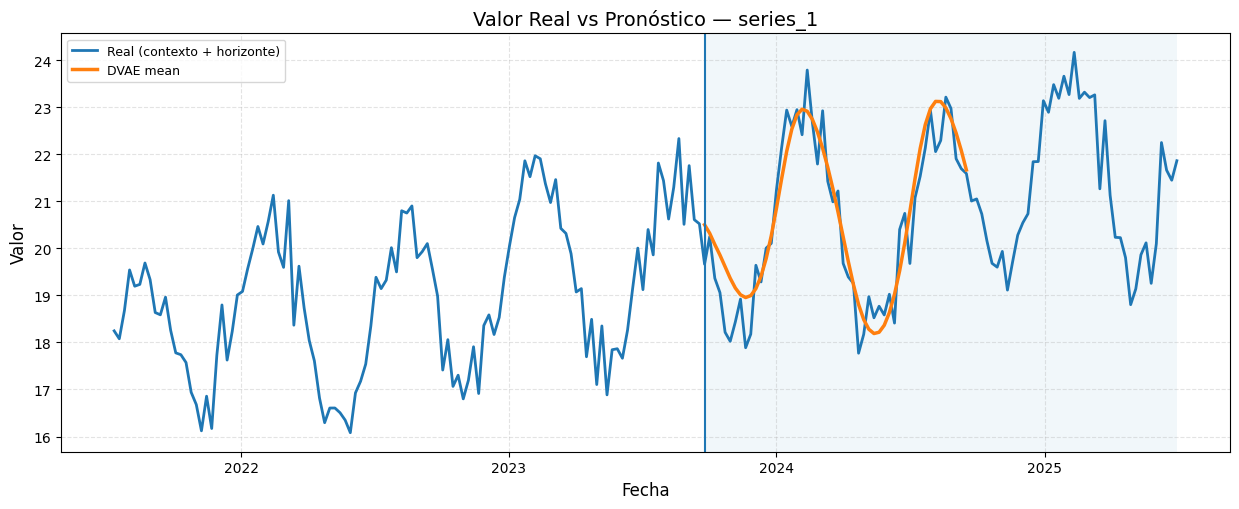
\includegraphics[width=1\linewidth]{dvae_fake_data.png}
    \caption{Valor real y pronóstico generado por el modelo D³VAE para una serie temporal sintética.}
    \label{fig:D3vae - pronostico de datos sintéticos}
\end{figure}

\subsubsection{Entrenamiento y Predicción}
Para reducir el efecto de incertidumbre, los autores \cite{li2022generative} proponen un proceso de difusión acoplada equipado con una red neuronal de reducción de ruido, sin tener que sacrificar la capacidad de generalización del modelo. Posteriormente, se realiza el desentrelazado de las variables latentes \( Z \) al minimizar la correlación total (TC), como se discutió previamente. Por último, los autores reconstruyeron la función de pérdida global utilizando todas las contribuciones previamente definidas, como se muestra...
\begin{equation}
    \mathcal{L} = \psi\cdot \mathcal{D}_{KL}\big( q(Y^{(t)}) || p_{\theta} (\hat{Y}^{(t)})\big) + \lambda\cdot L(\zeta,t)+\gamma\cdot L_{TC}+L_{\text{MSE}}\big( \hat{Y}^{(t)}, Y^{(t)} \big)
    \label{eq:loss_total}
\end{equation}
Donde, $L_{\text{MSE}}$ calcula el error cuadrado entre $\hat{Y}^{(t)}$ y $Y^{(t)}$, \( L(\zeta, t) \) corresponde a la pérdida de Scaled Denoising Score Matching (SDSM) y \( L_{\text{TC}} \) corresponde a la pérdida asociada al desentrelazado de las variables latentes. De esta manera el modelo generativo aprende al minimizar la función objetivo (\ref{eq:loss_total}).

\newpage
\section{Metodología}

Esta sección describe el pipeline metodológico implementado para pronosticar la inflación en México (INPC) y evaluar el efecto de distintas familias de variables exógenas y modelos. El enfoque compara tres configuraciones de entrada y dos protocolos de validación, utilizando la \textbf{optimización bayesiana} (BO) con \textbf{MAE} como métrica objetivo.

\subsection{Conjunto de datos y frecuencia}

El Índice Nacional de Precios al Consumidor (INPC) se obtiene del portal del INEGI en frecuencia quincenal y mensual.
Si bien la frecuencia mensual es la empleada oficialmente y la más habitual en la literatura económica, en esta investigación se adopta finalmente una \textbf{frecuencia semanal}, obtenida mediante una interpolación lineal a partir de los datos quincenales.

Esta decisión se fundamenta en que la \textbf{estructura fundamental del proceso inflacionario se mantiene} tras la desagregación temporal: las tendencias, ciclos y estacionalidades observadas en la versión mensual permanecen intactas, sin introducir ruido estructural significativo.
La granularidad adicional de la frecuencia semanal permite capturar variaciones de corto plazo y dinámicas transitorias que podrían pasar desapercibidas a nivel mensual.
En modelos neuronales, esta mayor densidad temporal mejora la sensibilidad del aprendizaje a cambios abruptos y a la estacionalidad de alta frecuencia, sin alterar la coherencia macroeconómica del fenómeno subyacente.
En consecuencia, se conserva la esencia del proceso inflacionario, pero se proporciona a los algoritmos una secuencia temporal más informativa y detallada.

De forma general, el \textbf{framework} desarrollado admite distintas configuraciones de frecuencia temporal según las características del conjunto de datos o el dominio de aplicación.
El usuario puede especificar la frecuencia mediante el parámetro \texttt{freq}, el cual acepta las siguientes opciones:
\begin{itemize}
    \item \texttt{"W-Mon"}: frecuencia \textbf{semanal}, con semanas iniciando en lunes (configuración por defecto utilizada en este estudio);
    \item \texttt{"ME"}: frecuencia \textbf{mensual}, que toma el último día de cada mes;
    \item \texttt{"B"}: frecuencia de \textbf{días hábiles} (\textit{Business Days}), útil para series financieras o de alta frecuencia.
\end{itemize}
Esta flexibilidad permite adaptar el sistema tanto a contextos macroeconómicos (como la inflación) como a dominios de ventas, producción o finanzas, manteniendo la consistencia de la estructura experimental.
%%\footnote{En la implementación, la frecuencia se define al inicializar el orquestador: \texttt{orquestador(freq="W-Mon")}.}

\subsection{Preprocesamiento y transformaciones}
Sea $y_t$ la serie de interés (inflación). En el experimento original, para estabilizar la dinámica y favorecer el aprendizaje en modelos neuronales se aplica \textbf{diferencia de orden 1} sobre la tasa de cambio (\(\Delta y_t\)), seguida de estandarización y reescalado. Todas las transformaciones se realizan con \textbf{anti-fuga}: sus parámetros se calculan exclusivamente con datos previos a cada ventana de validación.

El pipeline extendido descompone primero $y_t=\tau_t+c_t$. Las transformaciones \texttt{diff}, \texttt{diff\_logp1}, \texttt{pct}, \texttt{logp1}, \texttt{none} y \texttt{diff2} se permiten únicamente sobre $\tau_t$ y se invierten antes de reconstruir el pronóstico. El ciclo $c_t$ no se diferencia ni se transforma mediante logaritmos, debido a que puede tomar valores negativos; sólo se estandariza con la media y desviación del entrenamiento. Las variables de calendario y las componentes FFT se calculan por separado para cada componente y a partir de su respectiva historia.

\subsection{Ingeniería de variables}
Se estudian tres escenarios de covariables:
\begin{enumerate}[label=\Alph*.]
    \item \textbf{Target únicamente}: el modelo observa solo \(y_t\).
    \item \textbf{Target + temporales cíclicas}: se añaden codificaciones seno/coseno de \textit{mes}, \textit{trimestre} y \textit{día del mes} para capturar estacionalidad calendario.
    \item \textbf{Target + temporales cíclicas + FFT}: además de lo anterior, se incorporan \textbf{señales senoidales} derivadas de la \textit{Transformada Discreta de Fourier} aplicada al target. Se seleccionan las \(\text{top-}k\) componentes (aquí \(k=8\)) por energía, que se \textbf{extrapolan} al horizonte futuro para modelar periodicidades persistentes.
\end{enumerate}

\subsection{Modelos}
Se evaluaron: \textbf{Holt-Winters}, \textbf{XGBoost}, \textbf{RNN}, \textbf{LSTM}, \textbf{DeepAR} y \textbf{Transformer} (Vanilla). Cada modelo respeta la misma política de transformaciones y covariables por escenario. Para RNN, LSTM, DeepAR y Transformer se agregó una implementación propia en PyTorch con una interfaz común. RNN y LSTM emplean un codificador recurrente y una cabeza directa multihorizonte; DeepAR utiliza una LSTM autorregresiva con verosimilitud gaussiana; Transformer utiliza atención causal, codificación posicional y una cabeza multihorizonte. NeuralForecast se conserva únicamente para reproducir los experimentos históricos.

En el pipeline HP, cada arquitectura se instancia dos veces. Ambos modelos comparten el horizonte y el protocolo de validación, pero ajustan parámetros y escalas independientes para $\tau_t$ y $c_t$. El resultado evaluado no es cada componente de forma aislada, sino la serie reconstruida $\widehat{y}_t=\widehat{\tau}_t+\widehat{c}_t$.

\subsection{Protocolos de validación}
Se emplean dos esquemas complementarios:
\begin{itemize}
    \item \textbf{Validación simple (baseline)}: una partición con fecha de corte fija (\textit{single split}). Útil como línea base y para depuración.
    \item \textbf{Validación cruzada temporal (rolling-origin)}: se definen \(W\) ventanas \textbf{no solapadas} de \textbf{12 meses} (o tamaño elegido por el usuario), donde en cada ventana se re-entrena y evalúa el mismo modelo. Este protocolo reduce el sesgo por selección de una única partición y mide estabilidad en el tiempo.
\end{itemize}
La \textbf{métrica principal} es el \textbf{MAE}, por su interpretabilidad en niveles y su menor sensibilidad a valores atípicos en este caso de estudio.

\subsection{Optimización de hiperparámetros}
Para cada modelo y escenario de variables se utiliza \textbf{Optimización Bayesiana} con función objetivo:
\[
\theta^* \;=\; \arg\min_{\theta} \; \text{MAE}_{\text{val}}(\theta),
\]
donde \(\theta\) parametriza la arquitectura (p.~ej., número de capas/neuronas en RNN/LSTM; profundidad, \textit{learning rate} y rondas en XGBoost; cabezas/anchos en Transformer; estacionalidad en Holt-Winters). La BO balancea exploración/explotación mediante una función de adquisición (p.~ej., \textit{Expected Improvement}) y permite encontrar configuraciones competitivas con pocas evaluaciones.

\subsection{Protocolo de pronóstico final}
Una vez seleccionada \(\theta^*\) en cada ventana, el modelo se \textbf{re-entrena con toda la información disponible} previa al horizonte y se generan las predicciones. En el esquema \textit{single split}, para mantener consistencia con la validación, el pronóstico se produce desplazando \(-m\) meses según la ventana de validación definida por el usuario.

\subsection{Controles de sobreajuste y linealidad}
Además de la validación cruzada, se implementa un chequeo de \textbf{linealidad de pronósticos}: para una trayectoria \(\hat{y}_{t}\) (horizonte), se ajusta por mínimos cuadrados la recta \(m t + b\) y se calcula el \(\text{RMSE}(\hat{y}_t, m t + b)\). Si el RMSE cae por debajo de un umbral, la predicción se considera esencialmente lineal y se descarta como no informativa respecto a una regresión o promedio históricos. Este control evita aceptar configuraciones que \textit{aprenden} soluciones triviales.


\subsection{Diseño del experimento}
Se comparan los tres escenarios (A–C) en los horizontes de 6 y 12 meses, bajo ambos protocolos (baseline y rolling-origin). Para cada combinación (modelo, escenario, ventana) se realizan \(N\) iteraciones de BO (p.~ej., 20–30), reportando el \textbf{promedio} y la \textbf{dispersión} del MAE en validación cruzada. El mejor método se selecciona por MAE promedio y estabilidad (desviación estándar) a lo largo de las ventanas.

La extensión HP conserva estos horizontes y fechas de corte. Dentro de cada ventana se ejecutan, en orden, la descomposición restringida al entrenamiento, el ajuste de transformaciones y escalas, el entrenamiento independiente de los dos componentes, su inversión y la reconstrucción final. De esta forma, la comparación directa y la comparación HP utilizan exactamente los mismos valores reales y la misma métrica.

\subsection{Arquitectura del framework y reproducibilidad}
El sistema se implementa en Python con módulos desacoplados:
\begin{itemize}
    \item \textbf{Preprocesamiento} (\texttt{process\_data.py}, \texttt{utiles.py}): limpieza INEGI, re-muestreo, transformaciones, codificación temporal y generación de senoidales (FFT).
    \item \textbf{Funciones objetivo} (\texttt{obj\_bayes.py} y variantes \texttt{cv}): definen la pérdida (MAE), horizontes, frecuencias y \textit{anti-leakage}.
    \item \textbf{Ajuste} (\texttt{fit\_bayes\_opt.py} y \texttt{cross\_v*}): BO por modelo/escenario y por ventana (rolling).
    \item \textbf{Predicción} (\texttt{predict\_bayes.py}): re-entrena con \(\theta^*\) y produce \(\hat{y}\) fuera de muestra.
    \item \textbf{Orquestación} (\texttt{orquestador.py}, \texttt{main.py}): define \texttt{cutoff}, horizonte, métrica, frecuencia, iteraciones y ejecuta \texttt{train\_n\_predict()}; guarda métricas y predicciones.
\end{itemize}
El Anexo~\ref{anexo:codigo-rnn} presenta un ejemplo de la búsqueda bayesiana utilizada en el pipeline histórico.
La extensión se encuentra aislada en el paquete \texttt{inpc\_forecasting}. Sus módulos contienen la descomposición HP, transformaciones invertibles, ingeniería de variables por componente, modelos PyTorch y una interfaz de línea de comandos gobernada por YAML. Se fija la semilla 119, se habilita ejecución en CPU o GPU, se aplica detención temprana y recorte del gradiente, y se guarda un identificador de la configuración en cada archivo de resultados. Los módulos heredados con sufijo \texttt{cv} continúan implementando el protocolo histórico de validación cruzada temporal.

%%%%%%%%%%%%%%%%%%%%%%%%%%%%%%%%%%%%%%%%%%%%%%%%%%%%%%%%%%%%%%%%%%%%%%%%%%%%%%%%%%%%%%
\section{Resultados y discusión}

Esta sección resume los hallazgos experimentales del estudio comparativo. Se evaluaron dos
protocolos: (i) \textit{single split} como línea base y (ii) \textit{validación cruzada temporal}
(\textit{rolling-origin}) con ventanas de 12 meses. La métrica principal es el \textbf{MAE}
debido a su interpretabilidad en niveles y a que, en este caso de estudio, resulta menos sensible
a perturbaciones puntuales. Los resultados se reportan para horizontes de 6 y 12 meses.

\subsection{Diseño de evaluación}

Cada evaluación fija una fecha de corte, re-entrena el modelo con la información disponible hasta
dicho corte y evalúa el desempeño en el horizonte futuro. En el protocolo de validación cruzada,
este procedimiento se repite sobre múltiples ventanas temporales, lo que permite estimar el MAE
promedio y su dispersión. En consecuencia, la CV reduce el riesgo de conclusiones dependientes de
una única partición temporal y ofrece una estimación más estable del desempeño fuera de muestra.

\subsection{Escenarios de variables}

Se compararon tres configuraciones:
\begin{enumerate}[label=\Alph*.]
    \item \textbf{Target}: sólo \(y_t\).
    \item \textbf{Target + temporales cíclicas}: codificaciones sen/cos de \emph{mes}, \emph{trimestre} y \emph{día del mes}.
    \item \textbf{Target + temporales cíclicas + FFT}: además, \textbf{top-$k$} senoidales (en este trabajo \(k=8\)) obtenidas con DFT del target y extrapoladas al horizonte.
\end{enumerate}

\subsection{Línea base vs. validación cruzada}

La Tabla~\ref{tab:baseline_vs_cv} compara el MAE (media \(\pm\) sd) bajo \textit{single split} y
validación cruzada. El patrón general es consistente: el \textit{single split} tiende a producir
estimaciones más optimistas o más volátiles, mientras que la validación cruzada estabiliza la
medición al promediar múltiples cortes temporales. En particular, la dispersión del error entre
ventanas permite identificar modelos con desempeño robusto, en lugar de modelos favorecidos por un
único periodo de evaluación.

\begin{table}[H]
\centering
\caption{MAE (media \(\pm\) sd) por protocolo y horizonte.}
\label{tab:baseline_vs_cv}
\begin{tabular}{lcccc}
\toprule
\multirow{2}{*}{Modelo} & \multicolumn{2}{c}{6 meses} & \multicolumn{2}{c}{12 meses} \\
 & Single split & CV (12m) & Single split & CV (12m) \\
\midrule
Naive          & $0.5\pm0.28$ & $0.51\pm0.27$ & $0.58\pm0.27$ & $0.65\pm0.29$  \\
Promedio       & $0.45\pm0.24$ & $0.6\pm0.18$ & $0.5\pm0.18$ & $0.72\pm0.09$  \\
RWD            & $0.5\pm0.29$ & $0.53\pm0.17$ & $0.59\pm0.29$ & $0.6\pm0.2$ \\
Holt-Winters   & $1.6\pm0.95$ &  $0.97\pm1.02$  & $1.07\pm0$ & $1.22\pm1.4$ \\
XGBoost        & $0.79\pm0.7$ & $0.84\pm0.35$ & $1.08\pm 0.84$ & $0.76 \pm 0.14$ \\
RNN            & $0.53\pm0.24$ & $0.5 \pm 0.3$ & $0.66\pm0.4$ & $0.64\pm 0.38$  \\
LSTM           & $0.56\pm0.38$ & $0.51 \pm 0.32$ & $0.68\pm0.44$ & $0.65\pm0.35$  \\
DeepAR         & $0.54\pm0.4$ & $0.49 \pm 0.22$ & $0.56\pm0.34$ & $0.79\pm0.37$  \\
Transformer    & $0.65\pm0.32$ & $0.8 \pm 0.37$ & $0.82\pm0.42$ & $0.45\pm0.18$  \\
D$^3$VAE       & $0.54 \pm 0.24$ & $0.44 \pm 0.23$ & $0.48 \pm 0.11$ & $0.43 \pm 0.14$ \\
\bottomrule
\end{tabular}
\end{table}

\subsection{Impacto de las variables exógenas}

La Tabla~\ref{tab:vars_effect} reporta el MAE promedio en CV bajo los escenarios A/B/C. En
términos generales, incorporar variables temporales cíclicas tiende a mejorar el desempeño
respecto a usar únicamente el target, mientras que las senoidales FFT aportan valor adicional
cuando la serie presenta periodicidad marcada en el horizonte de evaluación. Sin embargo, el
efecto no es universal: en modelos altamente expresivos, añadir exógenas puede aumentar la
varianza o inducir sobreajuste dependiendo del protocolo y el horizonte.

\begin{table}[H]
\centering
\caption{MAE promedio (CV, 12m) por modelo y escenario de variables.}
\label{tab:vars_effect}
\begin{tabular}{lccc}
\toprule
Modelo & A) Target & B) Target+Temp & C) +FFT (k=8) \\
\midrule
Naive        & $0.65\pm0.29$ & -- & -- \\
Promedio     & $0.72\pm0.09$ & -- & -- \\
RWD          & $0.6\pm0.2$ & -- & -- \\
Holt-Winters & $1.22\pm1.4$ & -- & -- \\
XGBoost      & $0.76\pm 0.14$ & $0.80\pm 0.57$ & $0.87\pm 0.14$\\
RNN          & $0.64\pm 0.38$ & $0.77\pm 0.35$ & $0.88\pm0.77$ \\
LSTM         & $0.65\pm 0.35$ & $0.64\pm0.33$  & $0.74\pm0.47$ \\
DeepAR       & $0.79\pm 0.37$ & $0.84\pm0.34$  & $0.67\pm0.58$ \\
Transformer  & $0.45\pm 0.18$ & $0.76\pm0.29$  & $0.72\pm0.32$ \\
D$^3$VAE     & $0.43\pm 0.14$ & $0.58\pm 0.26$ & $0.59\pm 0.37$ \\
\bottomrule
\end{tabular}
\end{table}

\subsection{Ranking de modelos y estabilidad}

La Figura~\ref{fig:cv_model_comparison} sintetiza el ranking bajo validación cruzada, mostrando
MAE promedio y dispersión (sd). El criterio de selección final prioriza simultáneamente
\emph{bajo MAE} y \emph{baja variabilidad}. Bajo este criterio, D\textsuperscript{3}VAE presenta
el mejor desempeño y estabilidad global en ambos horizontes, mientras que Transformer destaca en
12 meses pero con mayor variación en 6 meses.

\begin{figure}[H]
    \centering
    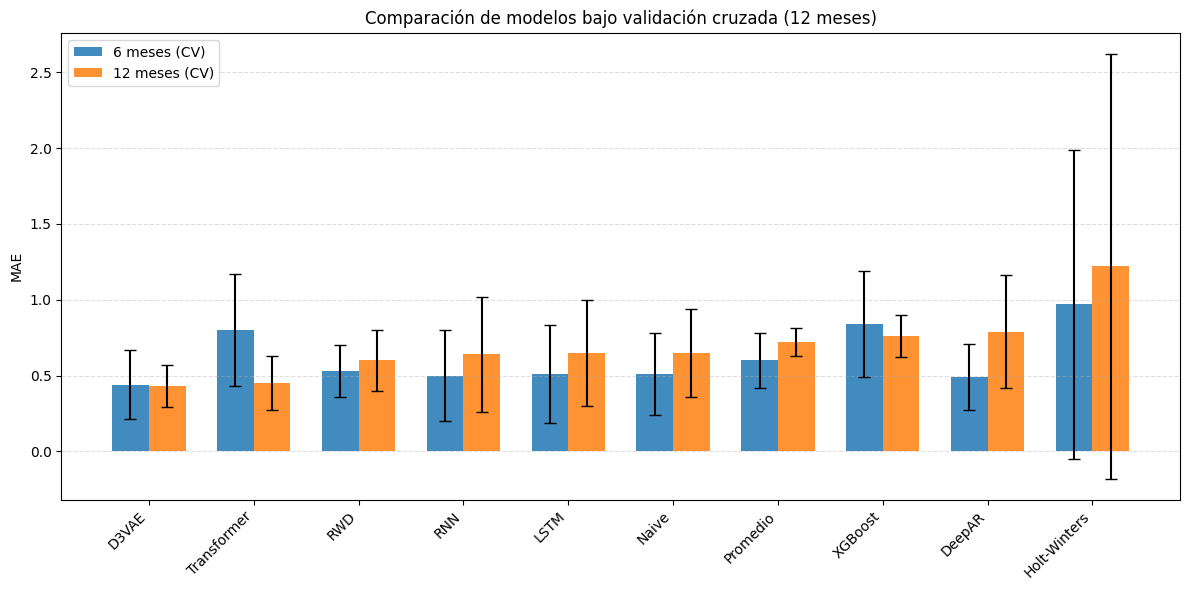
\includegraphics[width=1\linewidth]{ranking_modelos.png}
    \caption{Comparación del MAE bajo validación cruzada (12 meses) para horizontes de 6 y 12 meses. Las barras representan el promedio y las líneas verticales la desviación estándar.}
    \label{fig:cv_model_comparison}
\end{figure}

\subsection{Casos ilustrativos}

Para complementar el análisis agregado, se presentan ejemplos de pronóstico frente a valores
reales, con el fin de visualizar patrones de desempeño y fallas típicas (e.g., predicciones
lineales, sobreajuste al conjunto de validación). Las Figuras~\ref{fig:lstm_sens_best} y
\ref{fig:lstm_second_best_sens} muestran configuraciones representativas del comportamiento de
LSTM bajo distintas combinaciones de variables y suavizados.

\begin{figure}[H]
    \centering
    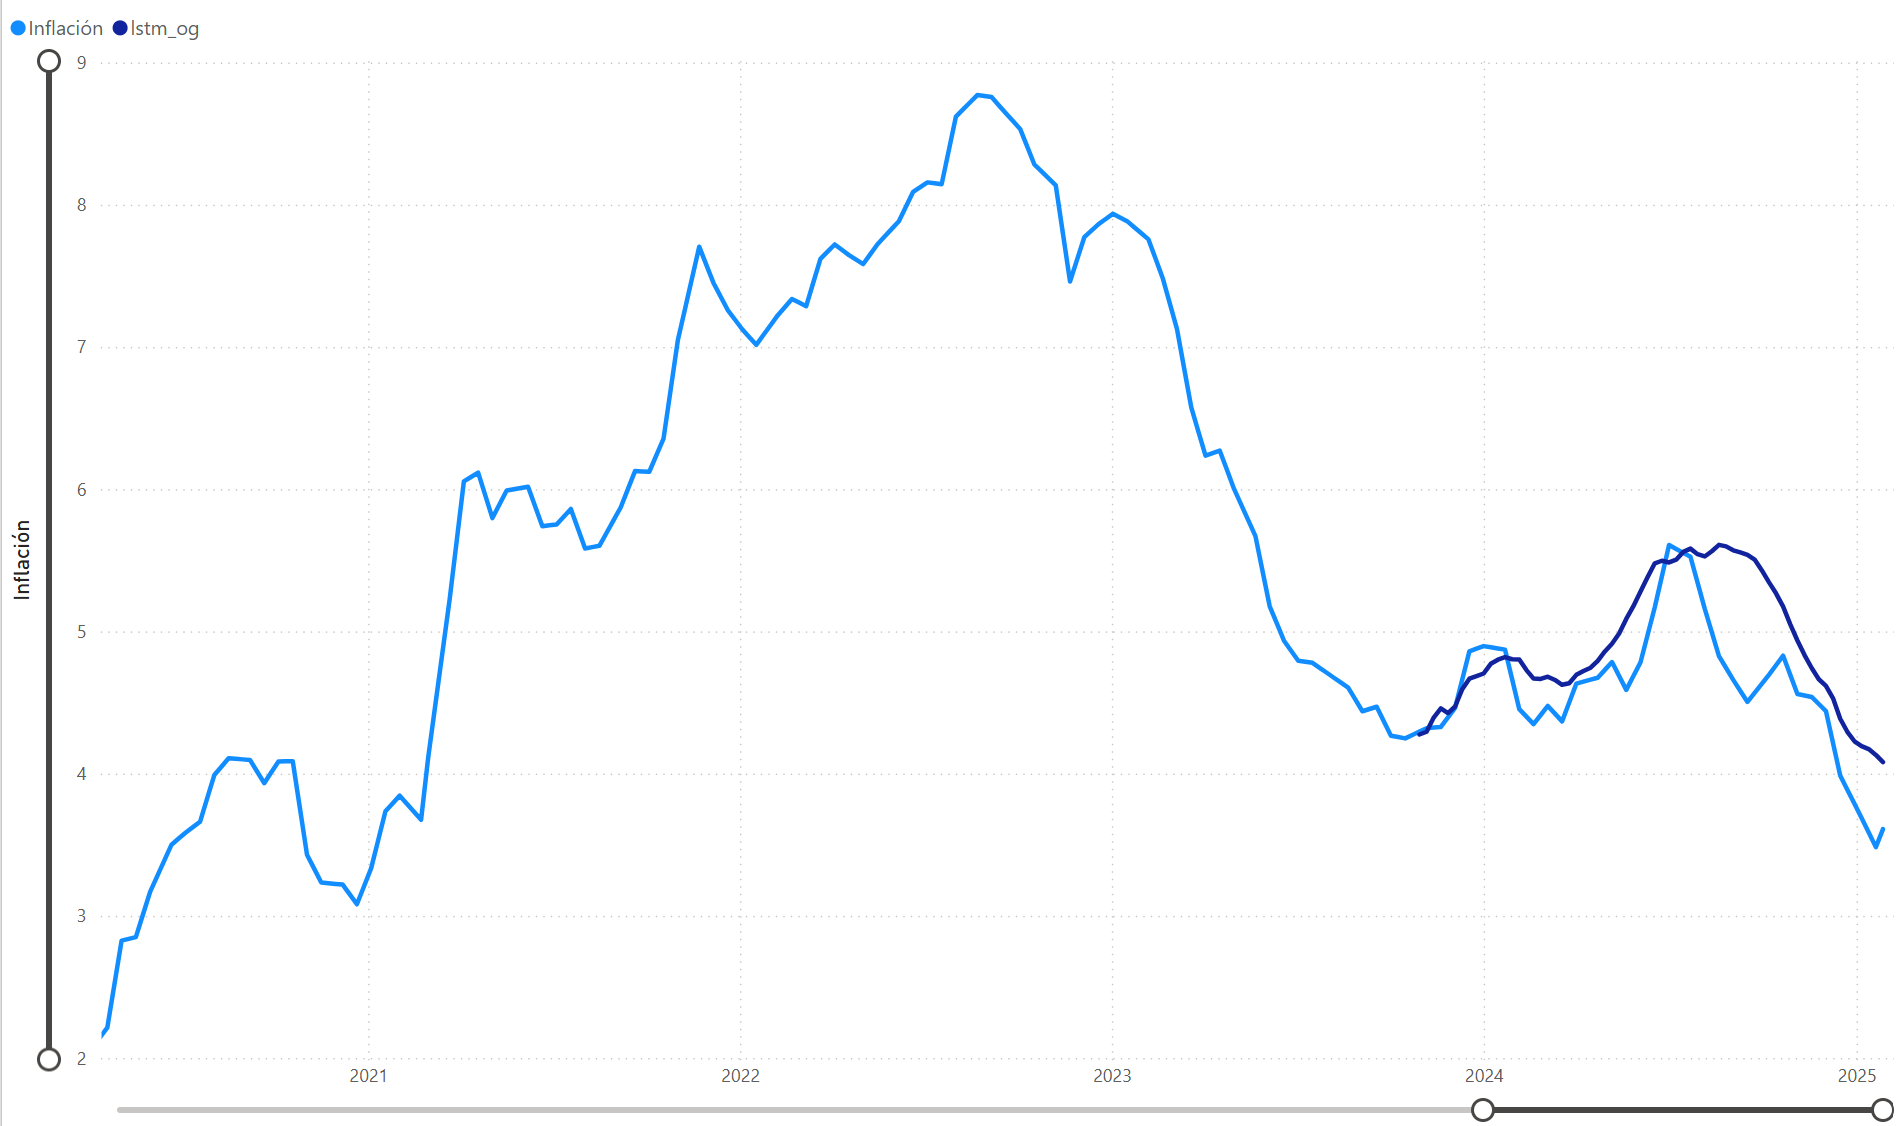
\includegraphics[width=0.8\textwidth]{lstm_good_one.png}
    \caption{Ejemplo ilustrativo de pronóstico con LSTM bajo una configuración de hiperparámetros optimizada.}
    \label{fig:lstm_sens_best}
\end{figure}

\begin{figure}[H]
    \centering
    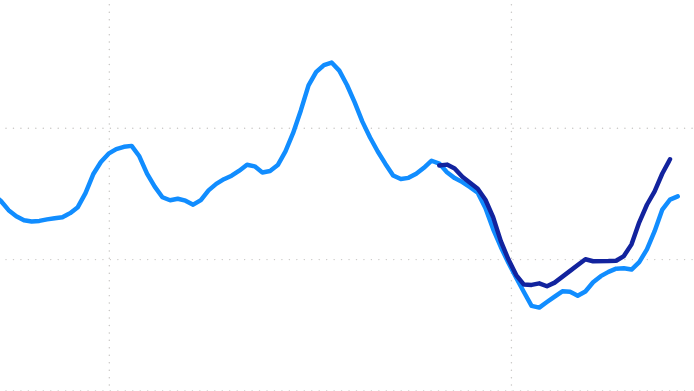
\includegraphics[width=0.8\textwidth]{second_Case.png}
    \caption{Ejemplo ilustrativo de pronóstico con LSTM incorporando suavizado exponencial para reducir ruido de alta frecuencia sin alterar la estructura general de la señal.}
    \label{fig:lstm_second_best_sens}
\end{figure}

\subsection{Control de linealidad}

Durante la optimización, se observó que ciertas configuraciones de redes neuronales (en particular
con arquitecturas excesivamente grandes) convergen a soluciones casi lineales en el horizonte,
lo cual constituye un comportamiento degenerado. Para detectar y penalizar estas soluciones, se
ajusta por mínimos cuadrados la recta \(mt+b\) a \(\hat{y}_t\) y se evalúa el error
\(\mathrm{RMSE}(\hat{y}_t, mt+b)\). Si el RMSE cae por debajo de un umbral, se aplica una
penalización fija al valor objetivo, forzando a la optimización bayesiana a explorar
configuraciones con dinámica no trivial. Este mecanismo evita aceptar configuraciones que no
superen a una regresión o a un promedio histórico.

\subsection{Discusión frente a la literatura}

Los resultados confirman que la complejidad de una arquitectura no garantiza por sí misma un menor error. Este comportamiento es consistente con la importancia de la estacionalidad señalada por \cite{capistran2009uso}: cuando la representación temporal no coincide con el horizonte o introduce redundancia, una red con mayor capacidad puede aumentar su varianza en lugar de mejorar su generalización. Del mismo modo, el desempeño competitivo de las líneas base obliga a interpretar las diferencias junto con su dispersión y no únicamente a partir del mejor valor observado en una ventana.

El mejor comportamiento de Transformer a doce meses es compatible con su capacidad para relacionar posiciones distantes mediante atención, mientras que la variabilidad de RNN y LSTM coincide con sus limitaciones para conservar dependencias largas, discutidas por \cite{sherstinsky2020fundamentals}. DeepAR aporta una formulación probabilística útil, pero su ventaja teórica no implica automáticamente una mejora en MAE cuando se dispone de una sola serie agregada; el modelo fue concebido para aprovechar conjuntos de series relacionadas \cite{salinas2020deepar}. Por otra parte, el desempeño de D\textsuperscript{3}VAE sugiere que representar incertidumbre y regularizar el espacio latente puede ser valioso, aunque esta conclusión permanece limitada a los cortes y horizontes evaluados.

\subsection{Extensión HP y resultados pendientes}

La implementación descrita en esta versión deja preparado el experimento que pronostica $\tau_t$ y $c_t$ de manera independiente con RNN, LSTM, DeepAR y Transformer propios. Sin embargo, una corrida mínima de verificación no es metodológicamente comparable con el benchmark completo. Por esta razón, no se sustituyen las métricas anteriores ni se afirma todavía que la descomposición HP reduzca el error. La hipótesis deberá evaluarse mediante todas las ventanas rolling-origin de seis y doce meses.

\begin{table}[H]
\centering
\caption{Matriz de resultados prevista para el benchmark HP. Los valores permanecen pendientes hasta ejecutar el protocolo completo.}
\label{tab:hp_pending}
\begin{tabular}{lcccc}
\toprule
Modelo & MAE 6 meses & sd 6 meses & MAE 12 meses & sd 12 meses \\
\midrule
RNN         & Pendiente & Pendiente & Pendiente & Pendiente \\
LSTM        & Pendiente & Pendiente & Pendiente & Pendiente \\
DeepAR      & Pendiente & Pendiente & Pendiente & Pendiente \\
Transformer & Pendiente & Pendiente & Pendiente & Pendiente \\
\bottomrule
\end{tabular}
\end{table}

\subsection{Hallazgos principales}

En conjunto, los resultados sustentan cuatro hallazgos principales:
\begin{itemize}
    \item La \textbf{validación cruzada temporal} produce estimaciones más estables y representativas que el \textit{single split}, reduciendo la dispersión del MAE entre ventanas.
    \item Las \textbf{transformaciones} para inducir estacionariedad fueron determinantes para evitar comportamientos triviales y estabilizar el entrenamiento, especialmente en modelos neuronales.
    \item Las \textbf{variables temporales cíclicas} no mejoran el desempeño respecto al escenario A en la mayoría de los modelos. Su efecto depende del horizonte y de la arquitectura: en algunos casos la red aprende información útil de estas covariables, pero el beneficio no se mantiene de manera consistente entre ventanas.
    \item En el ranking global bajo CV, \textbf{D\textsuperscript{3}VAE} presenta la mejor combinación de desempeño y estabilidad, mientras que \textbf{Transformer} destaca particularmente en el horizonte de 12 meses.
\end{itemize}

\section{Conclusiones}

En este trabajo se abordó el pronóstico de la inflación en México mediante un estudio comparativo
entre modelos clásicos, enfoques basados en árboles y arquitecturas neuronales (incluyendo modelos
probabilísticos y generativos). Los resultados muestran que, aunque los modelos simples ofrecen
líneas base competitivas, su desempeño y estabilidad dependen fuertemente del protocolo de
evaluación. En particular, la validación cruzada temporal fue esencial para obtener conclusiones
robustas y evitar selecciones guiadas por un único periodo histórico.

En relación con los objetivos planteados, se construyó el conjunto semanal del INPC, se estableció un protocolo común de comparación, se evaluaron transformaciones y variables temporales, y se integraron implementaciones propias de RNN, LSTM, DeepAR y Transformer. También quedó implementada la descomposición HP sin fuga temporal y el entrenamiento independiente de tendencia y ciclo. No obstante, la hipótesis específica sobre una reducción del MAE mediante esta descomposición permanece abierta: aceptarla o rechazarla requiere ejecutar el benchmark HP completo y no puede inferirse de las pruebas mínimas de funcionamiento.

A lo largo de la experimentación se observó que \textbf{la parsimonia} juega un papel central.
Reducir espacios paramétricos, limitar la complejidad de arquitecturas y controlar soluciones
degeneradas (como pronósticos casi lineales) mejoró la capacidad de generalización. Este hallazgo
es consistente con la práctica recomendada en el diseño de redes neuronales: comenzar con modelos
simples y aumentar complejidad únicamente cuando exista evidencia de mejora fuera de muestra.

En términos de variables, se encontró que las \textbf{codificaciones temporales cíclicas}
aportan información útil en la mayoría de escenarios, mientras que las \textbf{senoidales FFT}
pueden contribuir cuando la periodicidad es marcada, especialmente en horizontes más largos, aunque
su beneficio no es universal y la mayor parte de los experimentos lejos de tener un beneficio introdujo más ruido a los modelos.

Finalmente, bajo el criterio conjunto de \emph{bajo MAE} y \emph{baja variabilidad} en validación
cruzada, el modelo \textbf{D\textsuperscript{3}VAE} presentó el mejor desempeño global, seguido por
\textbf{Transformer} como alternativa competitiva en el horizonte de 12 meses. Estos resultados
sugieren que los enfoques generativos probabilísticos constituyen una vía prometedora para el
pronóstico inflacionario cuando se requiere modelar incertidumbre y obtener predicciones robustas
a diferentes ventanas temporales, mientras que el mejor desempeño del modelo Transformer puede
explicarse por su capacidad para modelar dependencias temporales de largo alcance de manera explícita.
A diferencia de arquitecturas recurrentes (RNN, LSTM) y de modelos autoregresivos probabilísticos
como DeepAR, el Transformer no comprime la información histórica en un estado oculto
secuencial, sino que accede directamente a todo el contexto de observaciones mediante
mecanismos de atención.

Como líneas de trabajo futuro, resulta natural extender este estudio en varias direcciones.
En primer lugar, considerar el modelado de múltiples componentes del índice inflacionario
permitiría analizar de forma más detallada la contribución de cada rubro al proceso agregado,
así como evaluar si ciertos modelos capturan mejor dinámicas sectoriales específicas.

En segundo lugar, resulta relevante estudiar periodos caracterizados por cambios estructurales
más pronunciados, como episodios de alta inflación, choques externos o modificaciones en la
política monetaria, con el fin de evaluar la robustez de los modelos ante rupturas en el
proceso generador de datos.

Asimismo, los resultados sugieren la necesidad de profundizar en estrategias que permitan
incorporar de manera más efectiva la información espectral obtenida mediante la descomposición
de Fourier. Si bien las senoidales dominantes aportan información estacional relevante, se
observó que su inclusión no siempre se traduce en una mejora consistente en la generalización.
Explorar mecanismos que permitan seleccionar, ponderar o regularizar estas señales de forma
adaptativa podría conducir a modelos más estables.

Un hallazgo particularmente interesante es que, en ciertos casos, arquitecturas como LSTM
logran modelar el proceso inflacionario con alta precisión cuando la estacionalidad es capturada
adecuadamente. Esto sugiere que el desafío no radica únicamente en la capacidad del modelo, sino
en lograr que la red neuronal aprenda la estructura estacional de forma efectiva y generalizable,
sin sobreajustarse a patrones específicos del conjunto de entrenamiento y validación.

Finalmente, se observó de manera consistente que la inclusión directa de variables temporales
explícitas (codificaciones de calendario) no mejoró el desempeño predictivo y, en muchos casos,
lo deterioró. Este comportamiento sugiere que dichas variables pueden introducir redundancia o
ruido cuando el modelo ya es capaz de inferir relaciones temporales a partir de la propia serie
y de representaciones espectrales. Este resultado refuerza la importancia de evaluar críticamente
la utilidad de las variables exógenas y de evitar su incorporación automática sin un análisis
previo de su impacto en la generalización.

\appendix
\section{Código de optimización para RNN}
\label{anexo:codigo-rnn}
\begin{lstlisting}[language=Python, caption={Búsqueda Bayesiana para RNN}, label={lst:fit_rnn}]
from bayes_opt import BayesianOptimization
from functools import partial
import pandas as pd

def fit_rnn(data, cutoff_date, iteraciones, freak, Metric, horizon, Mes_val, feats, transf, signals):
    rnn_params = {
        "years": (5, 12),
        "months": (Mes_val, Mes_val),
        "h": (horizon, horizon),
        "input_size": (6, 9),
        "neurons": (3, 4),
        "layers": (1, 2),
        "max_steps": (10, 70),
        "freq": (freq_map[freak], freq_map[freak]),
        "metric": (metric_map[Metric], metric_map[Metric]),
        "feats": (feats, feats),
        "signals": (signals, signals),
        "transf": (transformaciones_map[transf], transformaciones_map[transf]),
    }

    data = data.assign(ds=pd.to_datetime(data["ds"]))
    data = data[data["ds"] <= cutoff_date]

    rnn_objective = partial(obj_bayes.obj_rnn, data=data)

    opt = BayesianOptimization(
        f=rnn_objective,
        pbounds=rnn_params,
        random_state=119,
        verbose=2,
        allow_duplicate_points=False,
    )
    opt.maximize(init_points=3, n_iter=iteraciones)

    best = dict(opt.max["params"])
    best_score = opt.max["target"]   # p.ej., -MAE (mayor es mejor)
    return best, best_score
\end{lstlisting}


\bibliographystyle{plain}
\bibliography{refs}


\end{document}
